\chapter{Controller Design and Evaluation}
In this chapter, a control system is designed and evaluated to stabilize \glspl{flute} \gls{rf} system.
Referring back to the block diagram of a generic control system in \autoref{fig:theoreticalFramework-feedback-architecture}, there are three building blocks of a control system to be determined.
First the plant transfer function, which describes the system that is to be controlled.
Second, based on the plant, an appropriate controller type is chosen and its parameters are calculated.
Third, a measurement filter is used to improve the quality of the feedback signal path. As the choice of the measurement filter influences the controller design, its design is treated before the controller.

\section{Plant Identification}\label{sec:plantIdenti}
\subsection{Principle}
Before choosing an appropriate controller, some insight of the system response has to be obtained. Therefore in this section the plant's transfer function is estimated. In the context of this chapter ``plant'' refers to everything from the attenuation set at the controllable attenuator to the system output, e.g. the cavity \gls{rf} power.

In the time domain, a \gls{lti} system is described by its impulse response $h(t)$, that is the reaction of the plant to an impulse at the input.
Using this definition directly, the plant's impulse response $p(t)$ could be measured by applying a short peak in the attenuation setting on the attenuator. The effect on the output is not easy to measure and a single measurement of this kind is very susceptible to noise.
Therefore it is more common to measure the step response, which is the output of a system, when a step function is applied to its input. As the step function is the time integral of the impulse function, the step response can be converted to the impulse response by differentiation in time. \cite{Wang2000}

Instead of measuring a single step response, often several step responses are measured and their average is computed to reduce the variance of the estimation. When measuring a step response, the minimum needed measuring time depends on the systems time constants, but they are often not known beforehand.

That is why when there is no prior knowledge of the system, the identification is sometimes done with a \gls{prbs} to excite the system with step functions of different lengths. The \gls{prbs} is chosen in a way that some of the steps will probably last longer than a few dominant time constants of the system. 

To get the transfer function $P(s)=\mathcal{L}\left\{p(t)\right\}$ of the plant from its step response(s), several methods are common, including correlation based and frequency response based algorithms.

\subsection{Identifying the Plant Attenuator+RF}
The input \gls{prbs} signal is generated with the Python script in \autoref{lst:controllerDesignAndEvaluation-randomSequence}.
Based on the value of a pseudo random number generator, the sequence toggles the attenuator between $V_\text{control}=\SI{7}{\volt}$ and $V_\text{control}=\SI{11}{\volt}$.
Using \autoref{fig:interfacingFlute_attenDatten}, this equals a span in attenuation of \SIrange{6.892}{6.4026}{\dB}.
With the parameter \texttt{toggleP}, the average length of one constant voltage level can be controlled. 

\begin{lstlisting}[style=python,caption = Function to get a pseudo random binary sequence, label = lst:controllerDesignAndEvaluation-randomSequence]
def randomBinarySequence(N,toggleP):
    u=[False]*N
    for i in range(1,len(u)):
        if(np.random.binomial(1,toggleP,1)[0]):
            u[i]=not u[i-1]
        else:
            u[i]=u[i-1]
    return list(map(lambda x: 7 if x==False else 11,u))
\end{lstlisting}

In a test run over six hours (after all \gls{flute} subsystems had stabilized), the attenuator was driven with such a \gls{prbs}. The result is shown in \autoref{fig:controllerDesignAndEvaluation-identify-excitation}.

\begin{figure}[tb]
	\centering
	\includegraphics[width=\textwidth,height=0.5\textwidth]{chap/ControllerDesignAndEvaluation/img/identification/excitation.tikz}
	\caption[Identification sequence and response]{Section of the input sequence (blue, Attenuation) and the system response (orange, cavity RF power); Note the inverse relation: A higher attenuation $A$ causes a lower cavity power $P_\text{cavity}$}
	\label{fig:controllerDesignAndEvaluation-identify-excitation}
\end{figure}

The time signals $A(t)$ and $P_\text{cavity}(t)$ are then split into an \textit{estimation} data set (about \SI{80}{\percent} of the samples) and a \textit{validation} data set (the remaining $\approx$ \SI{20}{\percent}). This is done so the bulk of the available information is used to estimate the model, but there is data left that the model hasn't seen before. This smaller portion is used to validate the model's performance, hence it is called the validation data set.

The two data sets are then loaded into the \textsc{Matlab} \textit{System Identification Toolbox}. With the toolboxes pre-processing tools, first the means of both the input and output are removed, which is required by the estimators used.
Then, using the ``process model'' estimator, linear, continuous time transfer functions with different numbers of zeros and poles are estimated (See screenshot of the \gls{gui} in \autoref{fig:Appendix-identify}). After that, to check the accuracy of the estimations, the System Identification Toolbox is used to simulate the output of the estimated systems (see \autoref{fig:controllerDesignAndEvaluation-identify-mo}). For that the aforementioned validation data set is used. The measured output is compared with the outputs predicted by the models.

Using the Matlab function \texttt{zpk()} the models are converted into the zero-pole-gain representation. In
\autoref{tab:controllerDesignAndEvaluation-identify-models} the estimated models are listed with their zeros, poles, gains and the model fit, as it is computed by the System Identification Toolbox. \texttt{P1}, \texttt{P2} and \texttt{P3} are models with one, two and three poles and a gain as free parameters. \texttt{P2ZU} consists of a complex pole pair, a zero and a gain. 

\begin{figure}[tb]
	\centering
	\includegraphics[width=\textwidth,height=0.5\textwidth]{chap/ControllerDesignAndEvaluation/img/identification/modelOutputs.tikz}
	\caption[Validation of the process model]{Validation of the estimated process models for the plant; the legend also shows the model fits in percent}
	\label{fig:controllerDesignAndEvaluation-identify-mo}
\end{figure}

\begin{table}[tb]
\caption[Estimated process models]{Process models of the plant as estimated by the Matlab System Identification Toolboxes process model estimator}
\label{tab:controllerDesignAndEvaluation-identify-models}
\centering
\begin{tabular}{lcccc}
\toprule
Model & Zeros & Poles & Gain & Model fit \\
\midrule
P1   & & $(s+0.3505)$ & $-646.94$ & \SI{89.98}{\percent}\\
P2   & & $(s+0.6875) (s+0.7039)$ & $-873.18$ & \SI{93.83}{\percent}\\
P3   & & $(s+\num{1e06}) (s+0.7376) (s+0.669)$ & $\num{-8.9019e+08}$ & \SI{93.85}{\percent}\\
P2ZU &$(s-2846)$ & $(s^2 + 0.8014s + 0.3195)$ & $0.20296$ & \SI{96.26}{\percent}\\
\bottomrule
\end{tabular}
\end{table}

\autoref{fig:controllerDesignAndEvaluation-identify-mo} and \autoref{tab:controllerDesignAndEvaluation-identify-models} show the \texttt{P2ZU} model to have the best fit. Therefore it is accepted as the plants transfer function. Using the Matlab function \texttt{tf()}, its time continuous transfer function can be stated as
\begin{equation}
P(s) = \frac{0.6352s - 1808}{3.13 s^2 + 2.508 s + 1}.
\end{equation}
Using the Matlab function \texttt{c2d()}\footnote{Without specifying a different method, \texttt{c2d()}  discretizes the continuous-time model zero-order hold on the input.} and the sample time $T_s=\SI{0.2}{\second}$, $G(s)$ can be converted to the time discrete transfer function
\begin{equation}
P[z] = \frac{-10.91 z^{-1} - 10.41 z^{-2}}{1 - 1.84 z^{-1} + 0.8519 z^{-2}}.
\end{equation}

The high model fit percentage of \SI{96.26}{\percent} justifies the choice of a linear model with few parameters and further estimation attempts using other (non-) linear models are not needed.
Considering the accuracy of the model, it is important to note this estimation is only valid at the time the measurements are taken. With \gls{flute} being a large experimental setup still under commission, it is always possible that small changes to certain (sub-) systems can lead to minor or major influences to others.
For the time being, the estimation is redone a day later and for both measurements days, different parts of the about six hour measurements each are used as the estimation and validation data sets. Doing so shows no significant change in the estimated coefficients and the resulting model fits, indicating the estimated models are at least plausible.

To account for errors in the estimated model (and possible other errors), when designing the controller, sufficient gain and phase margins are set to ensure stable operation.










\newpage
\section{Measurement Filter}\label{sec:measurementFilter}
Like all measurements of physical quantities, the measuring of the system output of the control system is subjected to noise.
In addition to these disturbances of thermal or electrical origins, also high frequency variations of the system output have detrimental effects on the control systems performance.
For example, the magnitudes of the bunch-by-bunch changes of the measured cavity power are often in the same order as the long-term drifts.
Trying to correct for them, instead of the long term drifts, often leads to overcompensating and can even make the system unstable.

To remove the high frequency components, a low pass filter is used as the measurement block $H(s)$.

In pre-tests, the incoming signal was simply filtered with a moving average filter.
Commonly, the moving average is defined as the mean of a signal $x$ inside a window of length $L$, centered around the current time or sample index $n$, that is shifted along the signal. This smooths out small variations, thus the moving average acts as a low pass filter.
This \textit{non-causal} version of the moving average can only be used with already measured data as to compute the moving average at $n$, future values at $n+i$ are needed:
\begin{equation}
\operatorname{MA}_{x,\text{non-causal},L}[n] = \frac{1}{L} \sum_{i=n-\frac{L-1}{2}}^{n+\frac{L-1}{2}} x[i]
\end{equation}
When filtering real-time data, future values are not available and a shifted, \textit{causal} version, of the moving average
\begin{equation}\label{eq:causalMA}
\operatorname{MA}_{x,\text{causal},L}[n] = \frac{1}{L} \sum_{i=n-(L-1)}^{n} x[i]
\end{equation}
is used.

In case of the cavity \gls{rf} power, experiments show a window length of about $L=100$ or more is necessary to sufficiently smooth the measured power signal.
When comparing the original signal with the filtered one, it is apparent that in addition to the desired smoothing effect, the filtered signal also is delayed in time, with the delay being dependent on the window size.
To quantify the delay, the alternative definition of the moving average as a digital \gls{fir} filter is used.
One possibility to describe a \gls{fir} filter is by giving its impulse response, i.e. the output signal when the input of the filter is an impulse with unity height. In case of the moving average filter, the coefficient sequence of the corresponding \gls{fir} filter has the length $N=L$ and is equal to the the impulse response $h[n]$:
\begin{equation}
h[n] = \frac{1}{N} [\underbrace{1,\,1,\,...,\,1}_N]
\end{equation}

The delay introduced by a digital filter can be quantified with the filter's group delay
\begin{equation}
\frac{\tau_g(f)}{T_s} = \frac{\d{\phi(f)}}{\d{f}}
\end{equation}
which is given normalized to the sampling time $T_s$. \cite[p.~70]{Kammeyer2002} In case of a \gls{fir} filter with linear phase (with a symmetrical impulse response), the group delay is always constant over all frequencies and is only dependent on the filter length $N$ (see \cite[p.~165]{Kammeyer2002}):
\begin{equation}\label{eq:groupD}
\frac{\tau_g(f)}{T_s} = \frac{\d{\phi(f)}}{\d{f}} = \frac{\d{\phi}}{\d{f}} = \frac{N}{2}
\end{equation}

With a sampling time of $T_s=\nicefrac{1}{\SI{5}{\hertz}}=\SI{200}{\milli\second}$ and $N=100$ the group delay is \SI{10}{\second}. In case of a steady operation this is acceptable, as the disturbances to compensate happen on a timescale in the order of several minutes.
But in case of ongoing transients due to user changes to the control system parameters or short error bursts on the measured signal, this long delay causes problems and therefore should be reduced.

Therefore a more sophisticated digital filter is designed to replace the simple moving average.

On the one hand, a \gls{fir} filter is designed with the Kaiser window method.
This method starts with the desired frequency response, which is usually given piece-wise. 
In case of the low pass filter it is a step function at a cutoff frequency $f_c$.
Then the IDFT is used to compute the corresponding impulse response $h_\text{IIR}[n]$, which is in general infinitely long.
Windowing with e.g. a Kaiser window and then truncating the impulse response yields the impulse response of the desired \gls{fir} filter $h_\text{FIR}[n]$. \cite[p.~533]{Oppenheim2010}
With SciPy using \texttt{b=signal.firwin(N, fc,fs)}, the coefficients of a \gls{fir} with this method can be calculated.

On the other hand, an \gls{iir} filter is designed with the impulse invariance method and an analog Butterworth filter.
This method could be interpreted as sampling the infinitely long analog impulse response. \cite[p.~497]{Oppenheim2010}
In SciPy using \texttt{b,a=signal.butter(N,fc,'lowpass',fs,)}, the coefficients of an \gls{iir} can be calculated with this method.
For an \gls{iir} filter, the group delay cannot be calculated with \autoref{eq:groupD} and it is in general frequency-dependent.

\autoref{fig:controllerDesignAndEvaluation-impulseresponses} shows the impulse responses of the moving average, the \gls{fir} lowpass and the \gls{iir} lowpass (truncated to $N=100$).

\begin{figure}[tb]
	\centering
	\includegraphics[width=\textwidth,height=0.5\textwidth]{chap/ControllerDesignAndEvaluation/img/measurementFilter/firVsMa_impulseresponses.tikz}
	\caption[Impulse Responses of different time discrete filters]{Impulse responses of a moving average filter ($N=100$), a \gls{fir} lowpass ($N=50$, $f_c=\SI{0.1}{\hertz}$) and a \gls{iir} Butterworth lowpass ($N=50$, $f_c=\SI{0.1}{\hertz}$)}
	\label{fig:controllerDesignAndEvaluation-impulseresponses}
\end{figure}

In \autoref{fig:controllerDesignAndEvaluation-filterResults}, the three filter types described above are compared by filtering a ten minute long segment of pre-recorded data. The filtering is done with the SciPy function \texttt{signal.lfilter()} which does causal filtering and does not compensate group delay\footnote{In contrast to \texttt{signal.filtfilt()}, which applies the filter both forward and backward achieving zero phase/group delay, but this cannot be done for incoming real-time data.}, so the results are the same as they would be for real-time data.

\begin{figure}[tb]
	\centering
	\includegraphics[width=\textwidth,height=0.65\textwidth]{chap/ControllerDesignAndEvaluation/img/measurementFilter/firVsMa.tikz}
	\caption[Filter effects of different time discrete filters]{Effects of the three different lowpass filters in \autoref{fig:controllerDesignAndEvaluation-impulseresponses} on noisy data}
	\label{fig:controllerDesignAndEvaluation-filterResults}
\end{figure}

The plot shows the \gls{fir} lowpass filter requiring ten times the number of coefficients to achieve about the same result as the \gls{iir} lowpass filter.
Also the moving average filter has double the number of coefficients as the \gls{fir} lowpass filter, but there is still high frequency noise in the output (caused by the $\text{sinc}(\cdot)$ shape of its frequency response $H[f]=\operatorname{DFT}\{h[n]\}$).

Compared to the \gls{fir} lowpass, the moving average offers no benefit besides its easy implementation.
When comparing the \gls{fir} with the \gls{iir} approach, the \gls{iir} has the advantage of needing less coefficients, thus occupying less memory, which is not really an advantage when the control system is implemented on a personal computer, which typically has enough free memory to hold millions of floating point numbers.
Also the \gls{iir} filter has a non-constant group delay and is not guaranteed to be stable like all \gls{fir} filters are.

For these reasons, in the following a \gls{fir} lowpass filter is used.

One example filter generated with \texttt{signal.firwin()} with a cutoff frequency $f_c=\SI{10}{\milli\hertz}$ and order $N=10$ has the transfer function
\begin{equation}
H[z]=\frac{1}{b_{10} z^{10} + b_{9} z^9 + b_{8} z^8 + b_{7} z^7 + b_{6} z^6 + b_{5} z^5 + b_{4} z^4 + b_{3} z^3  + b_{2} z^2 + b_{1} z + b_{0}}
\end{equation}
with the coefficient vector $\vec{b}=[b_{10},\,...,\,b_0]$, with
\begin{equation}
\vec{b}=[0.0876,0.0896,0.0911,0.0922,0.0929,0.0931,0.0929,0.0922,0.0911,0.0896,0.0876].
\end{equation}

Instead of stating the transfer function, a plot of the poles and zeros is a more intuitive representation. In \autoref{fig:controllerDesignAndEvaluation-zplane}, the poles and zeros of the \gls{fir} filter with $N=10$ are compared to one with $N=40$. In addition, \autoref{fig:controllerDesignAndEvaluation-magn} shows the magnitude responses of such filters.

For a fixed cutoff frequency and variable order $N$, the trade-off for choosing $N$ is between the group delay introduced by the filter (see \autoref{eq:groupD}) and the width of the transition band or in other words the sharpness of the filter. This can be seen by comparing the cases $N=10$ and $N=40$ for the \gls{fir} filters in \autoref{fig:controllerDesignAndEvaluation-filterResults}: While the smoothing-effect of the longer filter is obviously better, it also causes a higher group delay, which results in the filter result of the $N=40$ filter being shifted in time by $\frac{40}{2}T_s = \SI{4}{\second}$ compared to $\frac{10}{2}T_s = \SI{1}{\second}$ in case of $N=10$. While a high smoothness is desired for the control system to reject high frequency noise, using a filter with a too high order can introduce a group delay high enough to shift the closed-loop from negative to positive feedback, thus making it unstable.

For the controller design in the next section and the later implemented real-time system, the cutoff frequency and the filter order are kept variable to leave room for improvement.

\begin{figure}[tb]
    \centering
        \subfloat[$N=10$]{% This file was created by matlab2tikz.
%
%The latest updates can be retrieved from
%  http://www.mathworks.com/matlabcentral/fileexchange/22022-matlab2tikz-matlab2tikz
%where you can also make suggestions and rate matlab2tikz.
%
\definecolor{mycolor1}{rgb}{0.00000,0.44700,0.74100}%
%
\begin{tikzpicture}

\begin{axis}[%
height=5cm,
width=5cm,
scale only axis,
xmin=-1.2,
xmax=1.2,
xlabel={Real Part},
ymin=-1.2,
ymax=1.2,
ylabel={Imaginary Part},
axis background/.style={fill=white},
title style={font=\bfseries},
]
\addplot [color=mycolor1, only marks, mark size=3, mark=o, mark options={solid, mycolor1}, forget plot]
  table[row sep=crcr]{%
0.836621499079625	0.547781404647655\\
0.836621499079625	-0.547781404647655\\
0.41185407563496	0.911249812281391\\
0.41185407563496	-0.911249812281391\\
-0.959594883641788	0.281385250659135\\
-0.959594883641788	-0.281385250659135\\
-0.655729055242191	0.75499629542878\\
-0.655729055242191	-0.75499629542878\\
-0.144472645356607	0.98950879467727\\
-0.144472645356607	-0.98950879467727\\
};
\addplot [color=mycolor1, only marks, mark size=3, mark=x, mark options={solid, mycolor1}, forget plot]
  table[row sep=crcr]{%
0	0\\
};
\draw[color=gray, dotted] (axis cs:0,0) circle[radius=1];
\node[above right, align=left]
at (axis cs:0.034,0) {(10)};
\end{axis}
\end{tikzpicture}
}
        \qquad
        \subfloat[$N=40$]{
\definecolor{color1}{rgb}{1,0.498039215686275,0.0549019607843137}

\begin{tikzpicture}

\begin{axis}[%
height=5cm,
width=5cm,
scale only axis,
xmin=-1.2,
xmax=1.2,
xlabel={Real Part},
ymin=-1.2,
ymax=1.2,
ylabel={Imaginary Part},
axis background/.style={fill=white},
title style={font=\bfseries},
]
\addplot [color=color1, only marks, mark size=3, mark=o, mark options={solid, color1}, forget plot]
  table[row sep=crcr]{%
0.987965884684059	0.154671945421421\\
0.987965884684059	-0.154671945421421\\
0.953087463195494	0.302695040427792\\
0.953087463195494	-0.302695040427792\\
0.895865695604845	0.444324943524943\\
0.895865695604845	-0.444324943524943\\
0.817641877278249	0.575727158053967\\
0.817641877278249	-0.575727158053967\\
0.720249516387962	0.693715095801514\\
0.720249516387962	-0.693715095801514\\
0.605971409373539	0.795486424159362\\
0.605971409373539	-0.795486424159362\\
0.477486138919954	0.878639281582218\\
0.477486138919954	-0.878639281582218\\
0.337805291172425	0.941216014130611\\
0.337805291172425	-0.941216014130611\\
0.190202866963389	0.981744808694656\\
0.190202866963389	-0.981744808694656\\
0.0381385420949963	0.999272461147043\\
0.0381385420949963	-0.999272461147043\\
-0.997066265180957	0.0765432089613322\\
-0.997066265180957	-0.0765432089613322\\
-0.973699583531299	0.227835732559618\\
-0.973699583531299	-0.227835732559618\\
-0.927513915445789	0.373788625635431\\
-0.927513915445789	-0.373788625635431\\
-0.859591813840491	0.510981324099441\\
-0.859591813840491	-0.510981324099441\\
-0.77152531521101	0.636198623064017\\
-0.77152531521101	-0.636198623064017\\
-0.665378623646589	0.74650605301911\\
-0.665378623646589	-0.74650605301911\\
-0.543639727636105	0.839318679963541\\
-0.543639727636105	-0.839318679963541\\
-0.114823424494493	0.993385917550353\\
-0.114823424494493	-0.993385917550353\\
-0.409162083727107	0.912461719328592\\
-0.409162083727107	-0.912461719328592\\
-0.265097733923631	0.964221546880464\\
-0.265097733923631	-0.964221546880464\\
};
\addplot [color=color1, only marks, mark size=3, mark=x, mark options={solid, color1}, forget plot]
  table[row sep=crcr]{%
0	0\\
};
\draw[color=gray, dotted] (axis cs:0,0) circle[radius=1];
\node[above right, align=left]
at (axis cs:0.034,0) {(40)};
\end{axis}
\end{tikzpicture}
}
       \caption[FIR pole zero maps]{Pole-Zero maps for two \gls{fir} filters with a common cutoff frequency $f_c=\SI{10}{\milli\hertz}$ but different filter orders $N$;\\ $\circ$ denotes zeros, $\times$ denotes poles, $(k)$ is a $k$-times pole}
    \label{fig:controllerDesignAndEvaluation-zplane}
\end{figure}

\begin{figure}[tb]
	\centering
	\includegraphics[width=\textwidth,height=0.6\textwidth]{chap/ControllerDesignAndEvaluation/img/measurementFilter/lpFiltMagnitude.tikz}
	\caption[FIR magnitude response]{Magnitude response of two \gls{fir} filters with a common cutoff frequency $f_c=\SI{10}{\milli\hertz}$ but different filter orders $N$}
	\label{fig:controllerDesignAndEvaluation-magn}
\end{figure}

\FloatBarrier
\paragraph{Real-time implementation of a FIR Filter in Python}
Similar to \autoref{eq:causalMA}, a \gls{fir} filter designed with the SciPy function \texttt{sigal.firwin()} can be used in a causal manner to filter real-time data.

Applying the filter on pre-recorded data, like in \autoref{fig:controllerDesignAndEvaluation-filterResults} can be done with \texttt{signal.lfilter()}. To use \texttt{signal.lfilter()} on sample-wise incoming real-time data, the ``initial in'' input and ``final out'' output of \texttt{signal.lfilter()} can be used to keep the filters state. This is demonstrated in \autoref{lst:controllerDesignAndEvaluation-zizf} by looping through pre-recorded data point-by-point.

\begin{lstlisting}[style=python,caption = Demonstration of the \texttt{zi} and \texttt{zf} variables when using \texttt{signal.lfilter()}, label = lst:controllerDesignAndEvaluation-zizf]
x=df2["F:RF:LLRF:01:GunCav1:Power:Out Value"].to_numpy()
y=np.array([])
zf=signal.lfilter_zi(b, 1)
for i in range(len(x)):
    y0,zf=signal.lfilter(b, 1, [x[i]],zi=zf)
    y=np.append(y,y0[0])
\end{lstlisting}











\newpage
\section{Controller Design}
Based on the estimated model of the plant $P(s)$ (or $P[z]$) in \autoref{sec:plantIdenti} and the type of measurement filter designed in \autoref{sec:measurementFilter}, in this section an appropriate controller to stabilize the plant is designed and its performance is evaluated.

Tuning the controller and testing its capabilities is performed both \textit{offline} with simulations using the building blocks $P[z]$, $H[z]$ and the yet to be defined $G[z]$ and \textit{online} using a software implementation of the control system with the real hardware, i.e. \gls{flute} and the controllable attenuator.

\subsection{Choosing a Controller Type}
The plant has been identified using a linear model in \autoref{sec:plantIdenti} resulting in the \gls{lti} system $P(s)$ (or $P[z]$). The matching controller does not necessarily have to be a \gls{lti} system, but choosing a \gls{lti} system simplifies design and analysis and is a justifiable choice here, as there are no good reasons against it, yet.

The class of \gls{lti} controllers is dominated by the \gls{pid} controller and its variants. \gls{pid} stands for ``proportional'', ``integral'' and ``derivative'', which are \gls{lti} systems themselves, performing scaling, integration or differentiation. Depending on the application, variants, such as the PI controller, or the PD controller are used as well.

According to \cite[p.~111]{Aastroem1995} \gls{pid} control is applicable for plants with order two or less.
Compared to other types of controllers, using a \gls{pid} controller has many advantages. It is is quick to design and does not depend on an accurate plant model. Also after the designing step, the few free parameters can easily be presented to an operator and online fine tuning is possible.\footnote{In contrast a compensating controller is based on an accurate model of the plant and changes on the fly are difficult. \cite{SergeZacher2010}}

In the next section such a \gls{pid} controller is designed. As it is to be implemented in software later, the design is done in discrete time.

\subsection{Designing a Discrete Time PID Controller}\label{sec:controlDesign}
The output signal $u(t)$ of a generic time continuous \gls{pid} controller (see \autoref{fig:controllerDesignAndEvaluation-genericPID}) consists of the weighted sum of three error signals.

\begin{figure}[tb]
	\centering
	\includegraphics[width=0.8\textwidth]{chap/ControllerDesignAndEvaluation/img/controller/pid.tikz}
	\caption[Block diagram of a PID controller]{Block diagram of a generic \gls{pid} controller}
	\label{fig:controllerDesignAndEvaluation-genericPID}
\end{figure}
The first is simply the controller input error signal $e(t)$ scaled by the gain $k_p$. This is the proportional part of the \gls{pid} controller. The integral part is calculated by computing the running time integral
\begin{equation}\label{eq:ei}
e_i(t)=\int_{0}^{t} e(\tau) \d{\tau}.
\end{equation}
This is then scaled by the constant $k_i$. To get the derivative part, the derivative
\begin{equation}\label{eq:ed}
e_d(t)=\frac{\d{}}{\d{t}} e(t)
\end{equation}
is calculated and weighted with $k_d$.
All three are then summed to get $u(t)$ in the so called parallel form (see \cite[p.~5]{Dodds2015}):
\begin{equation}
u(t)=k_p e(t) + k_i \int_{0}^{t} e(\tau) \d{\tau} + k_d \frac{\d{}}{\d{t}} e(t)
\end{equation}
Often instead of the parallel form, the \gls{pid} controller is stated in \textit{standard form}. Instead of using the gains $k_{p,\,i,\,d}$, the parameters proportional gain $K$, integral time $T_i$ and derivative time $T_d$ are used. \cite[p.~76]{Aastroem1995} With the conversions
\begin{align}
K&=k_i\\
T_i=\frac{k_p}{k_i}&=\frac{K}{k_i}\\
T_d=\frac{k_d}{k_p}&=\frac{k_d}{K}
\end{align}
the \gls{pid} controller in standard form is
\begin{equation}
u(t)=K\left[e(t) + \frac{1}{T_i} \int_{0}^{t} e(\tau) \d{\tau} + T_d \frac{\d{}}{\d{t}} e(t)\right].
\end{equation}
The transfer function $G(s)$ is given by the Laplace of $u(t)$ using the computation rules (see \cite{Leon2015})
\begin{align}
\mathcal{L}\left\{\int_{0}^{t} y(\tau) \d{\tau}\right\} &= \frac{1}{s} Y(s)\\
\mathcal{L}\left\{\frac{\d{}}{\d{t}} y(t)\right\} &= s Y(s)
\end{align}
as
\begin{equation}
G(s)=K\left[1+\frac{1}{s T_i}+s T_d\right].
\end{equation}
To get the discrete transfer function, either the Laplace transform $G(s)=\nicefrac{U(s)}{E(s)}$, is discretized or the $\mathcal{Z}$ transform of $u[n]$ is calculated.
First, to get $u[n]$, the derivative in \autoref{eq:ed} is approximated by
\begin{equation}
e_d[n]=\frac{e[n]-e[n-1]}{T_s}.
\end{equation}
This assumes $e(t)$ is sampled with a sampling rate of $f_s=\nicefrac{1}{T_s}$ to get $e[n]$. In a similar fashion, the integral in \autoref{eq:ei} is approximated by
\begin{equation}
e_i[n]=e_i[n-1] + e[n] T_s.
\end{equation}

Using the shift rule of the $\mathcal{Z}$ transform (see \cite{Leon2015})
\begin{equation}
y[n-k] \laplace z^{-k} Y[z],
\end{equation}
the discrete transfer function of the \gls{pid} controller is
\begin{equation}
G[z]=K\left[1+\frac{T_s}{T_i}\frac{z}{z-1}+\frac{T_d}{T_s}\frac{z-1}{z}\right].
\end{equation}
In the time domain, this becomes
\begin{equation}\label{eq:pidn}
u[n] = k_p e[n] 
+ k_i \left(\underbrace{e_i[n-1] + T_s e[n]}_{e_i[n]}\right) 
+ k_d \left(\underbrace{\frac{1}{T_s} e[n]-e[n-1]}_{e_d[n]}\right)
\end{equation}

\subsubsection{Controller Tuning}
Next the three free parameters $k_{p,\,i,\,d}$ or $K,\,T_{i,\,d}$ are to be chosen in such a way that the controller has optimal performance. This process is called \textit{tuning}. Tuning of the parameters can be performed online or offline.

Online tuning is done by using the physical\footnote{``Physical'' in the sense that one could touch it. (But should one?)} plant. The most popular member of this class is the Ziegler-Nichols tuning. The method relies on experiments and tabulated values. The mostly used variant uses one measured step response. \cite{Ziegler1942}

Using this method at \gls{flute} produced mixed results. While being a very simple and fast process, the resulting controller is often unstable. This is partially due to errors when extracting the tabulated values from the noisy step response, but also the method intrinsically leads to poor stability margins. \cite[p.~142]{Aastroem1995}
Nonetheless the Ziegler-Nichols method yields a usable starting point, if the strategy is to fine tune the controller manually by intuition and experience of the user.

As the Ziegler-Nichols method does not yield an acceptable parameter set and the method combined with fine tuning by hand takes a considerable amount of time, next tuning the parameters offline using only the plants transfer function and the measurement filter is done.
The offline tuning can be done analytically or using different numerical optimization strategies. In \cite{DiazRodriguez2019} analytical methods, such as the internal model control design or the pole placement design are discussed. Both require the system's transfer function in a closed form.\\
Tuning by numerical optimization chooses the parameters by a simulation or measured data. Goal of the optimization is to minimize a cost function $J$ like
\begin{equation}
J(\theta) = \sum_{n=0}^{\infty} e_{\theta}[n]^2
\end{equation}
with the parameter vector $\theta=[k_p,\,k_i,\,k_d]$ or $\theta=[K,\,T_i,\,T_d]$:
\begin{equation}
\theta_\text{opt} = \underset{\theta}{\text{argmin}} J(\theta)
\end{equation}

A convenient way to do such an optimization by simulation using the transfer function of the estimated plant is the Matlab \textit{PID Tuner}.

\paragraph{Offline Tuning the Controller with the Matlab PID Tuner}
The Matlab \gls{pid} Tuner accepts different kinds of system models used by the Matlab/Simulink ecosystem. It is possible to directly use estimated models, models defined via their transfer function or the zero-pole-gain representation, Simulink models or combinations of those\footnote{Series connection can be established by multiplying the models transfer functions.}.

The manual of the PID Tuner (see \cite{pidTunerMan}) describes the expected input (see \autoref{fig:controllerDesignAndEvaluation-pidTunersys}). The feedback path has to have unity gain, i.e. there is no measurement filter allowed. Therefore the measurement filter is moved before the junction where the output $y[n]$ would normally be measured. Then the measurement filter $H[z]$ is combined with the plant $P[z]$ to form $Sys[z]$. For that reason $y[n]$ becomes an internal signal of $Sys[z]$. However the new system output $y'[n]=h[z] \ast y[n]$ is not too different from the old one, since $H[z]$ is designed to remove high frequency noise but retain the rest of $y[n]$.

\begin{figure}[tb]
	\centering
	\includegraphics[]{chap/ControllerDesignAndEvaluation/img/controller/pidTunerArch.tikz}
	\caption[System architecture for the Matlab PID tuner]{Required system architecture for the Matlab PID Tuner; PID Tuner input is the system block $Sys[z]$ (green), generated output is the controller $G[z]$ (blue)}
	\label{fig:controllerDesignAndEvaluation-pidTunersys}
\end{figure}

The manufacture's documentation in \cite{pidTuner} does not disclose any internals of the PID Tuner nor state which optimization technique is used, but three tuning objectives are stated:
\begin{itemize}
\item Stability: The closed loop should be stable (that is BIBO stable as defined in \autoref{def:bibo})
\item Performance: The closed loop system tracks the input well and rejects disturbances as rapidly as possible (see \autoref{sec:drandtrack})
\item Robustness: A gain and phase margin accounts for errors in the system model (see \autoref{sec:plantIdenti})
\end{itemize}

Using \autoref{lst:controllerDesignAndEvaluation-pidTuner}, the estimated plant $P[z]$ is loaded, a measurement filter $H[z]$ is generated and the combination $Sys[z]=P[z]H[z]$ is fed into the PID Tuner.

\begin{lstlisting}[style=matlab,caption = Matlab script to generate an input system for PID Tuner, label = lst:controllerDesignAndEvaluation-pidTuner]
% design lowpass measurement filter H
N=10;
lpFilt1 = designfilt('lowpassfir', 'FilterOrder', N, 'CutoffFrequency', ...
                    0.01, 'SampleRate', 0.2, 'DesignMethod', ...
                    'window', 'Window', 'kaiser');

% convert filter to a dynamic system                
[z1,p1,k1]=zpk(lpFilt1);
H1=zpk(z1,p1,k1,0.2);

% load estimated transfer function and convert it to discrete form
load('P2ZU.mat')
P=c2d(idtf(P2ZU),0.2);

Sys1=tf1*H1; %Combine plant P and measurement filter H
pidTuner(Sys1); %Launch pidTuner
\end{lstlisting}

Using the PID Tuner \gls{gui} (see \autoref{fig:Appendix-pidTuner}), the controller is designed by changing the design parameters \texttt{Response Time} (RT) and \texttt{Transient Behavior} (TB). Changing the response time (in seconds) influences how fast the controller acts on changes. With the transient behavior setting, the allowed over- and under-shoots, that is, the deviation above and below the final value for $t \rightarrow \infty$ can be set qualitatively.

With this tool four different controllers are designed, two for each measurement filter's order of $N=10$ and $N=40$. The transient behavior with $0.2$ for all controllers is chosen as a compromise between speed and overshoot behavior. The optimized \gls{pid} parameters (for a discrete time \gls{pid} controller in parallel form) are listed in \autoref{tab:controllerDesignAndEvaluation-pidTunerResults}.

\begin{table}[tb]
\caption[Calculated PID parameters]{Parameters of a discrete time \gls{pid} controller in parallel form calculated with the Matlab PID Tuner; $N$ is the order of the used measurement filter}
\label{tab:controllerDesignAndEvaluation-pidTunerResults}
\centering
\begin{tabular}{lSSSSSS}
\toprule
Name & {$N$} & {RT (in \si{\second})} & {TB} & {$k_p$} & {$k_i$} & {$k_d$} \\
\midrule
$G_1[z]$ &10 & 5   & 0.2 & \num{-0.000577} & \num{-0.000197} & \num{-0.000421}\\
$G_2[z]$ &10 & 10  & 0.2 & \num{-0.000155} & \num{-0.000111} & \num{-5.43e-05}\\
$G_3[z]$ &40 & 5   & 0.2 & \num{-0.000559} & \num{-2.27e-05} & \num{-0.000396}\\
$G_4[z]$ &40 & 10  & 0.2 & \num{-0.00035} & \num{-9.68e-05} & \num{-0.000316}\\
\bottomrule
\end{tabular}
\end{table}

\subsection{Analyzing the Input Tracking and Disturbance Rejection}
The PID Tuner defaults to show the input tracking step response (as in \autoref{fig:Appendix-pidTuner}).
The input tracking is calculated based on \autoref{eq:inputTracking}. To calculate it, the Matlab function \texttt{step()} is used, which generates the step response plot of a dynamic system, in this case $F_T$. As the whole system only consists of linear building blocks, using an arbitrary step height of $1$ is possible. The response is then normalized in such a way that the final value is also $1$.

In \autoref{fig:controllerDesignAndEvaluation-pidTunerITN10} and \autoref{fig:controllerDesignAndEvaluation-pidTunerITN40} the input tracking step responses for all four controllers are plotted. Note the different $t$ scales. As expected, for longer measurement filters, i.e. filters of higher orders, the controller has to act less aggressive. This causes longer settling times.
Especially \autoref{fig:controllerDesignAndEvaluation-pidTunerITN40} shows that setting a shorter response time does not automatically cause the controller to set the output faster to its final value. While for the shorter response time, the set value is reached quicker, there is also a strong oscillation, so choosing the longer response time (see $G_4[z]$) can be beneficial.

\begin{figure}[tb]
	\centering
	\includegraphics[width=\textwidth,height=0.6\textwidth]{chap/ControllerDesignAndEvaluation/img/controller/pidTuner/trackingN10.tikz}
	\caption[Input tracking of controller one and two]{Step response of the input tracking $F_T$ for controller $G_1[z]$ and $G_2[z]$, designed with the plant $P[z]$ and a measurement filter of order $N=10$, response time goal to \SI{5}{\second} and \SI{10}{\second}}
	\label{fig:controllerDesignAndEvaluation-pidTunerITN10}
\end{figure}

\begin{figure}[tb]
	\centering
	\includegraphics[width=\textwidth,height=0.6\textwidth]{chap/ControllerDesignAndEvaluation/img/controller/pidTuner/trackingN40.tikz}
	\caption[Input tracking of controller three and four]{Step response of the input tracking $F_T$ for controller $G_3[z]$ and $G_4[z]$, designed with the plant $P[z]$ and a measurement filter of order $N=40$, response time goal to \SI{5}{\second} and \SI{10}{\second}}
	\label{fig:controllerDesignAndEvaluation-pidTunerITN40}
\end{figure}

As the set-point for \gls{flute} only changes occasionally, basically a fixed set-point controller is needed. Therefore the disturbance rejection is more important than the input tracking when analyzing the controllers performance. The step responses of the disturbance rejection $F_{DR}$ are calculated in a similar way as the input tracking, using \autoref{eq:disturbanceRejection} and \texttt{step()}. The $y$ axes are normalized so that the initial value is $1$ and the final value for $t \rightarrow \infty$ is $0$.

In \autoref{fig:controllerDesignAndEvaluation-pidTunerDRN10} and \autoref{fig:controllerDesignAndEvaluation-pidTunerDRN40} the results for all controllers in \autoref{tab:controllerDesignAndEvaluation-pidTunerResults} are plotted.

This shows that even for an optimistically low measurement filter order of $N=10$, the settling time is in the order of slightly under a minute. This is sufficient for the application, but has more of a practical drawback: when fine-tuning the \gls{pid} parameters manually on the machine, it is necessary to wait a few minutes after setting new parameters before assessing the change.

Especially when looking a the plots of $G_3[z]$, it is obvious that there can be stability issues when using a too aggressive controller. For that reason in the next section the stability of the four controllers is analyzed.

\begin{figure}[tb]
	\centering
	\includegraphics[width=\textwidth,height=0.6\textwidth]{chap/ControllerDesignAndEvaluation/img/controller/pidTuner/rejectionN10.tikz}
	\caption[Disturbance rejection of controller one and two]{Step response of the disturbance rejection $F_{DR}$ for controller $G_1[z]$ and $G_2[z]$, designed with the plant $P[z]$ and a measurement filter of order $N=10$, response time goal to \SI{5}{\second} and \SI{10}{\second}}
	\label{fig:controllerDesignAndEvaluation-pidTunerDRN10}
\end{figure}

\begin{figure}[tb]
	\centering
	\includegraphics[width=\textwidth,height=0.6\textwidth]{chap/ControllerDesignAndEvaluation/img/controller/pidTuner/rejectionN40.tikz}
	\caption[Disturbance rejection of controller three and four]{Step response of the disturbance rejection $F_{DR}$ for controller $G_3[z]$ and $G_4[z]$, designed with the plant $P[z]$ and a measurement filter of order $N=40$, response time goal to \SI{5}{\second} and \SI{10}{\second}}
	\label{fig:controllerDesignAndEvaluation-pidTunerDRN40}
\end{figure}


\subsection{Analyzing the Controller Stability}
In this section the stability of the controllers $G_{i}[z]$ from the last section is evaluated.

For that the Nyquist criterion according to \autoref{def:Nyquist} is used. With the Matlab function \texttt{nyquist()}, the locus $w=F_o[w=j2\pi f]$ of the open loops
\begin{equation}
F_o[z]=G[z] P[z] H[z]
\end{equation}
are calculated. For all controllers designed, they are plotted in \autoref{fig:controllerDesignAndEvaluation-pidTunerNyq}.

This shows the gain margin for $G_3[z]$ (in combination with the $N=40$ filter), that is the distance to the critical point $w=(-1,0j)$, is already very small. So in addition to its oscillatory behavior and the longer settling time, there is also the risk that the system can become unstable if there are even small system parameter changes.

\begin{figure}[tb]
	\centering
	\includegraphics[]{chap/ControllerDesignAndEvaluation/img/controller/pidTuner/nyquist1.tikz}
	\caption[Nyquist plot for all controllers]{Nyquist plot to analyze the stability of the closed-loop control system based on the locus plot of the open-loop system; Note the critical point $(-1,\,0j)$ is always on ``left'' of the curve indicating stability}
	\label{fig:controllerDesignAndEvaluation-pidTunerNyq}
\end{figure}

In \autoref{fig:controllerDesignAndEvaluation-pidTunerfails} another issue is highlighted. If a controller is designed with a certain measurement filter order $N=N_0$ in mind, but is used together with a filter of order $N=N_1>N_0$, it is very likely the closed loop system becomes unstable. In the figure the controller $G_1[z]$ is used together with the $N=40$ filter. Both the disturbance rejection and the Nyquist plot show the closed loop to be unstable.

\begin{figure}[tb]
    \centering
        \subfloat[Step response of the disturbance rejection; amplitude of oscillations grow over time]{% This file was created by matlab2tikz.
%
%The latest updates can be retrieved from
%  http://www.mathworks.com/matlabcentral/fileexchange/22022-matlab2tikz-matlab2tikz
%where you can also make suggestions and rate matlab2tikz.
%
\definecolor{mycolor1}{rgb}{0.00000,0.44700,0.74100}%
%
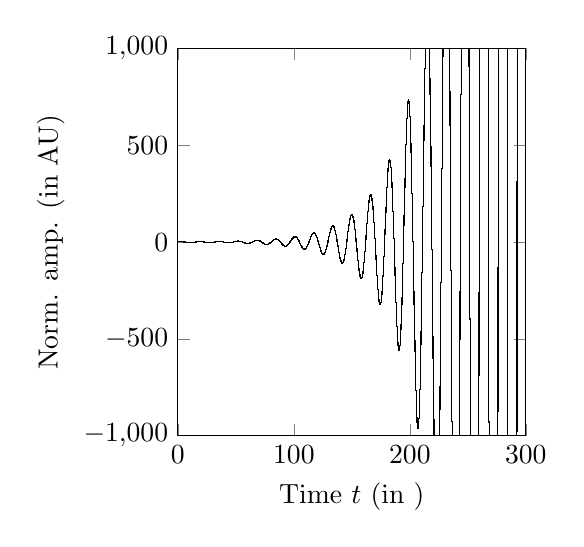
\begin{tikzpicture}

\begin{axis}[%
width=6cm,
height=6.5cm,
xmin=0,
xmax=300,
ymin=-1000,
ymax=1000,
xlabel={Time $t$ (in \si{\second})},
ylabel={Norm. amp. (in AU)},
axis background/.style={fill=white},
legend style={legend cell align=left, align=left, draw=white!15!black}
]
\addplot [color=black, forget plot]
  table[row sep=crcr]{%
0	1\\
0.2	1\\
0.2	1.00012375593908\\
0.4	1.00012375593908\\
0.4	1.00062966128937\\
0.6	1.00062966128937\\
0.6	1.00179500474329\\
0.8	1.00179500474329\\
0.8	1.00388796592845\\
1	1.00388796592845\\
1	1.00713695281658\\
1.2	1.00713695281658\\
1.2	1.0116995490953\\
1.4	1.0116995490953\\
1.4	1.0176335097753\\
1.6	1.0176335097753\\
1.6	1.02487221956032\\
1.8	1.02487221956032\\
1.8	1.03320680588593\\
2	1.03320680588593\\
2	1.04227668722496\\
2.2	1.04227668722496\\
2.2	1.05156977150307\\
2.4	1.05156977150307\\
2.4	1.06043282447789\\
2.6	1.06043282447789\\
2.6	1.06809179281304\\
2.8	1.06809179281304\\
2.8	1.07368109315941\\
3	1.07368109315941\\
3	1.07628020927715\\
3.2	1.07628020927715\\
3.2	1.07495533406585\\
3.4	1.07495533406585\\
3.4	1.06880340292951\\
3.6	1.06880340292951\\
3.6	1.05699563479635\\
3.8	1.05699563479635\\
3.8	1.03881772038534\\
4	1.03881772038534\\
4	1.013704007101\\
4.2	1.013704007101\\
4.2	0.981263481172466\\
4.4	0.981263481172466\\
4.4	0.941295935056831\\
4.6	0.941295935056831\\
4.6	0.89379743987126\\
4.8	0.89379743987126\\
4.8	0.838955025436776\\
5	0.838955025436776\\
5	0.777131249455833\\
5.2	0.777131249455833\\
5.2	0.708840070546827\\
5.4	0.708840070546827\\
5.4	0.63471602052559\\
5.6	0.63471602052559\\
5.6	0.555479119235314\\
5.8	0.555479119235314\\
5.8	0.471898190968326\\
6	0.471898190968326\\
6	0.384755263610507\\
6.2	0.384755263610507\\
6.2	0.294813533276512\\
6.4	0.294813533276512\\
6.4	0.202790982848838\\
6.6	0.202790982848838\\
6.6	0.109341208911485\\
6.8	0.109341208911485\\
6.8	0.0150423505139146\\
7	0.0150423505139146\\
7	-0.079605668835819\\
7.2	-0.079605668835819\\
7.2	-0.174176080721734\\
7.4	-0.174176080721734\\
7.4	-0.268303484467825\\
7.6	-0.268303484467825\\
7.6	-0.36166695061688\\
7.8	-0.36166695061688\\
7.8	-0.453969953743966\\
8	-0.453969953743966\\
8	-0.544919265367201\\
8.2	-0.544919265367201\\
8.2	-0.634094314927572\\
8.4	-0.634094314927572\\
8.4	-0.720944227708456\\
8.6	-0.720944227708456\\
8.6	-0.804898968894809\\
8.8	-0.804898968894809\\
8.8	-0.885378187988563\\
9	-0.885378187988563\\
9	-0.961800632361883\\
9.2	-0.961800632361883\\
9.2	-1.03359367476534\\
9.4	-1.03359367476534\\
9.4	-1.10020253419988\\
9.6	-1.10020253419988\\
9.6	-1.16109881355673\\
9.8	-1.16109881355673\\
9.8	-1.21578806395697\\
10	-1.21578806395697\\
10	-1.26381615975818\\
10.2	-1.26381615975818\\
10.2	-1.30477436990571\\
10.4	-1.30477436990571\\
10.4	-1.3383031031752\\
10.6	-1.3383031031752\\
10.6	-1.36409437846163\\
10.8	-1.36409437846163\\
10.8	-1.38189316210892\\
11	-1.38189316210892\\
11	-1.39149774395107\\
11.2	-1.39149774395107\\
11.2	-1.39275937787664\\
11.4	-1.39275937787664\\
11.4	-1.3855814109758\\
11.6	-1.3855814109758\\
11.6	-1.36991812594983\\
11.8	-1.36991812594983\\
11.8	-1.34577348796204\\
12	-1.34577348796204\\
12	-1.31319996352342\\
12.2	-1.31319996352342\\
12.2	-1.27229750488779\\
12.4	-1.27229750488779\\
12.4	-1.22321277588357\\
12.6	-1.22321277588357\\
12.6	-1.1661386063919\\
12.8	-1.1661386063919\\
12.8	-1.10131364883335\\
13	-1.10131364883335\\
13	-1.02902214764355\\
13.2	-1.02902214764355\\
13.2	-0.949593725535894\\
13.4	-0.949593725535894\\
13.4	-0.863403056155252\\
13.6	-0.863403056155252\\
13.6	-0.77086932182715\\
13.8	-0.77086932182715\\
13.8	-0.672455321278759\\
14	-0.672455321278759\\
14	-0.568666170454216\\
14.2	-0.568666170454216\\
14.2	-0.460047502502741\\
14.4	-0.460047502502741\\
14.4	-0.347183165360961\\
14.6	-0.347183165360961\\
14.6	-0.230692395488453\\
14.8	-0.230692395488453\\
14.8	-0.111226514966462\\
15	-0.111226514966462\\
15	0.010534806825125\\
15.2	0.010534806825125\\
15.2	0.133887642518852\\
15.4	0.133887642518852\\
15.4	0.258108176289216\\
15.6	0.258108176289216\\
15.6	0.382457258434643\\
15.8	0.382457258434643\\
15.8	0.506185072176976\\
16	0.506185072176976\\
16	0.628535839257302\\
16.2	0.628535839257302\\
16.2	0.748752508446677\\
16.4	0.748752508446677\\
16.4	0.86608140204942\\
16.6	0.86608140204942\\
16.6	0.979776815664497\\
16.8	0.979776815664497\\
16.8	1.08910556703151\\
17	1.08910556703151\\
17	1.19335147990169\\
17.2	1.19335147990169\\
17.2	1.29181979194406\\
17.4	1.29181979194406\\
17.4	1.38384147522115\\
17.6	1.38384147522115\\
17.6	1.46877745756361\\
17.8	1.46877745756361\\
17.8	1.54602273237376\\
18	1.54602273237376\\
18	1.61501033625087\\
18.2	1.61501033625087\\
18.2	1.67521518405717\\
18.4	1.67521518405717\\
18.4	1.72615772626215\\
18.6	1.72615772626215\\
18.6	1.76740742142717\\
18.8	1.76740742142717\\
18.8	1.79858597834668\\
19	1.79858597834668\\
19	1.81937036068412\\
19.2	1.81937036068412\\
19.2	1.82949550781136\\
19.4	1.82949550781136\\
19.4	1.82875676202744\\
19.6	1.82875676202744\\
19.6	1.81701196363617\\
19.8	1.81701196363617\\
19.8	1.79418320092139\\
20	1.79418320092139\\
20	1.7602581884952\\
20.2	1.7602581884952\\
20.2	1.71529126304954\\
20.4	1.71529126304954\\
20.4	1.65940397554688\\
20.6	1.65940397554688\\
20.6	1.59278528419873\\
20.8	1.59278528419873\\
20.8	1.51569131955615\\
21	1.51569131955615\\
21	1.42844475221926\\
21.2	1.42844475221926\\
21.2	1.33143372037641\\
21.4	1.33143372037641\\
21.4	1.22511037208316\\
21.6	1.22511037208316\\
21.6	1.10998897166817\\
21.8	1.10998897166817\\
21.8	0.986643635405466\\
22	0.986643635405466\\
22	0.855705654013396\\
22.2	0.855705654013396\\
22.2	0.71786045867473\\
22.4	0.71786045867473\\
22.4	0.573844210666386\\
22.6	0.573844210666386\\
22.6	0.424440053651452\\
22.8	0.424440053651452\\
22.8	0.27047403235685\\
23	0.27047403235685\\
23	0.112810704521159\\
23.2	0.112810704521159\\
23.2	-0.0476515361032569\\
23.4	-0.0476515361032569\\
23.4	-0.209985400603876\\
23.6	-0.209985400603876\\
23.6	-0.373239885028807\\
23.8	-0.373239885028807\\
23.8	-0.536445663991024\\
24	-0.536445663991024\\
24	-0.698620664722512\\
24.2	-0.698620664722512\\
24.2	-0.858775798640085\\
24.4	-0.858775798640085\\
24.4	-1.01592080766206\\
24.6	-1.01592080766206\\
24.6	-1.16907020461747\\
24.8	-1.16907020461747\\
24.8	-1.3172492593064\\
25	-1.3172492593064\\
25	-1.45950000897816\\
25.2	-1.45950000897816\\
25.2	-1.59488724276914\\
25.4	-1.59488724276914\\
25.4	-1.72250443754705\\
25.6	-1.72250443754705\\
25.6	-1.84147959506108\\
25.8	-1.84147959506108\\
25.8	-1.9509809556489\\
26	-1.9509809556489\\
26	-2.0502225424513\\
26.2	-2.0502225424513\\
26.2	-2.13846950715315\\
26.4	-2.13846950715315\\
26.4	-2.21504323819547\\
26.6	-2.21504323819547\\
26.6	-2.27932620048273\\
26.8	-2.27932620048273\\
26.8	-2.33076646836186\\
27	-2.33076646836186\\
27	-2.36888193333847\\
27.2	-2.36888193333847\\
27.2	-2.39326413287642\\
27.4	-2.39326413287642\\
27.4	-2.40358170813901\\
27.6	-2.40358170813901\\
27.6	-2.39958342168484\\
27.8	-2.39958342168484\\
27.8	-2.38110075389257\\
28	-2.38110075389257\\
28	-2.34805002315672\\
28.2	-2.34805002315672\\
28.2	-2.30043403107841\\
28.4	-2.30043403107841\\
28.4	-2.23834320823122\\
28.6	-2.23834320823122\\
28.6	-2.1619562493237\\
28.8	-2.1619562493237\\
28.8	-2.07154022322921\\
29	-2.07154022322921\\
29	-1.96745015883857\\
29.2	-1.96745015883857\\
29.2	-1.85012809191649\\
29.4	-1.85012809191649\\
29.4	-1.72010157421046\\
29.6	-1.72010157421046\\
29.6	-1.57798166089086\\
29.8	-1.57798166089086\\
29.8	-1.42446034514237\\
30	-1.42446034514237\\
30	-1.260307501701\\
30.2	-1.260307501701\\
30.2	-1.08636729158055\\
30.4	-1.08636729158055\\
30.4	-0.903554093071041\\
30.6	-0.903554093071041\\
30.6	-0.712847945537727\\
30.8	-0.712847945537727\\
30.8	-0.515289536624118\\
31	-0.515289536624118\\
31	-0.311974764275225\\
31.2	-0.311974764275225\\
31.2	-0.1040488841385\\
31.4	-0.1040488841385\\
31.4	0.107299710132471\\
31.6	0.107299710132471\\
31.6	0.320846055883227\\
31.8	0.320846055883227\\
31.8	0.53533549494607\\
32	0.53533549494607\\
32	0.749490820353507\\
32.2	0.749490820353507\\
32.2	0.962019653314415\\
32.4	0.962019653314415\\
32.4	1.17162201214256\\
32.6	1.17162201214256\\
32.6	1.37699802675839\\
32.8	1.37699802675839\\
32.8	1.57685575878077\\
33	1.57685575878077\\
33	1.76991907589609\\
33.2	1.76991907589609\\
33.2	1.95493554116855\\
33.4	1.95493554116855\\
33.4	2.13068426060323\\
33.6	2.13068426060323\\
33.6	2.29598365337899\\
33.8	2.29598365337899\\
33.8	2.44969908214822\\
34	2.44969908214822\\
34	2.59075031216234\\
34.2	2.59075031216234\\
34.2	2.71811873558995\\
34.4	2.71811873558995\\
34.4	2.83085432906104\\
34.6	2.83085432906104\\
34.6	2.9280822874548\\
34.8	2.9280822874548\\
34.8	3.00900929795229\\
35	3.00900929795229\\
35	3.07292940550288\\
35.2	3.07292940550288\\
35.2	3.11922943636589\\
35.4	3.11922943636589\\
35.4	3.14739392832155\\
35.6	3.14739392832155\\
35.6	3.15700955257858\\
35.8	3.15700955257858\\
35.8	3.14776896506074\\
36	3.14776896506074\\
36	3.11947408691073\\
36.2	3.11947408691073\\
36.2	3.07203876302935\\
36.4	3.07203876302935\\
36.4	3.00549078302151\\
36.6	3.00549078302151\\
36.6	2.91997325487263\\
36.8	2.91997325487263\\
36.8	2.81574528368457\\
37	2.81574528368457\\
37	2.69318198699187\\
37.2	2.69318198699187\\
37.2	2.5527737881602\\
37.4	2.5527737881602\\
37.4	2.39512502551748\\
37.6	2.39512502551748\\
37.6	2.22095184687676\\
37.8	2.22095184687676\\
37.8	2.03107940861026\\
38	2.03107940861026\\
38	1.82643837676772\\
38.2	1.82643837676772\\
38.2	1.60806075510966\\
38.4	1.60806075510966\\
38.4	1.37707503450024\\
38.6	1.37707503450024\\
38.6	1.134700711902\\
38.8	1.134700711902\\
38.8	0.882242174606921\\
39	0.882242174606921\\
39	0.621082002822607\\
39.2	0.621082002822607\\
39.2	0.352673701874124\\
39.4	0.352673701874124\\
39.4	0.0785339216993929\\
39.6	0.0785339216993929\\
39.6	-0.199765822535246\\
39.8	-0.199765822535246\\
39.8	-0.48060785456089\\
40	-0.48060785456089\\
40	-0.762337452359199\\
40.2	-0.762337452359199\\
40.2	-1.04327229438737\\
40.4	-1.04327229438737\\
40.4	-1.32171221047071\\
40.6	-1.32171221047071\\
40.6	-1.5959491624168\\
40.8	-1.5959491624168\\
40.8	-1.86427741265698\\
41	-1.86427741265698\\
41	-2.1250038111053\\
41.2	-2.1250038111053\\
41.2	-2.37645814844613\\
41.4	-2.37645814844613\\
41.4	-2.617003507081\\
41.6	-2.617003507081\\
41.6	-2.84504655545929\\
41.8	-2.84504655545929\\
41.8	-3.05904771342144\\
42	-3.05904771342144\\
42	-3.25753113688411\\
42.2	-3.25753113688411\\
42.2	-3.43909444830443\\
42.4	-3.43909444830443\\
42.4	-3.60241815983128\\
42.6	-3.60241815983128\\
42.6	-3.74627472269738\\
42.8	-3.74627472269738\\
42.8	-3.86953714776718\\
43	-3.86953714776718\\
43	-3.97118713130463\\
43.2	-3.97118713130463\\
43.2	-4.05032264946432\\
43.4	-4.05032264946432\\
43.4	-4.10616493447651\\
43.6	-4.10616493447651\\
43.6	-4.13806483032648\\
43.8	-4.13806483032648\\
43.8	-4.14550842703994\\
44	-4.14550842703994\\
44	-4.12812198049049\\
44.2	-4.12812198049049\\
44.2	-4.08567603834993\\
44.4	-4.08567603834993\\
44.4	-4.01808876766308\\
44.6	-4.01808876766308\\
44.6	-3.92542842330735\\
44.8	-3.92542842330735\\
44.8	-3.80791497110754\\
45	-3.80791497110754\\
45	-3.66592078497919\\
45.2	-3.66592078497919\\
45.2	-3.49997048373231\\
45.4	-3.49997048373231\\
45.4	-3.31073979569154\\
45.6	-3.31073979569154\\
45.6	-3.09905355473298\\
45.8	-3.09905355473298\\
45.8	-2.86588272351054\\
46	-2.86588272351054\\
46	-2.61234053521643\\
46.2	-2.61234053521643\\
46.2	-2.33967770440647\\
46.4	-2.33967770440647\\
46.4	-2.0492767578773\\
46.6	-2.0492767578773\\
46.6	-1.74264549292893\\
46.8	-1.74264549292893\\
46.8	-1.42140959581418\\
47	-1.42140959581418\\
47	-1.08730444854954\\
47.2	-1.08730444854954\\
47.2	-0.742166172158901\\
47.4	-0.742166172158901\\
47.4	-0.38792193567311\\
47.6	-0.38792193567311\\
47.6	-0.0265795948527464\\
47.8	-0.0265795948527464\\
47.8	0.339783300236508\\
48	0.339783300236508\\
48	0.709031058633614\\
48.2	0.709031058633614\\
48.2	1.07898191309756\\
48.4	1.07898191309756\\
48.4	1.44742051844488\\
48.6	1.44742051844488\\
48.6	1.81211082304229\\
48.8	1.81211082304229\\
48.8	2.17080923973614\\
49	2.17080923973614\\
49	2.52127803166597\\
49.2	2.52127803166597\\
49.2	2.86129885544397\\
49.4	2.86129885544397\\
49.4	3.1886863547404\\
49.6	3.1886863547404\\
49.6	3.50130175380339\\
49.8	3.50130175380339\\
49.8	3.79706633982881\\
50	3.79706633982881\\
50	4.07397477627471\\
50.2	4.07397477627471\\
50.2	4.33010814788125\\
50.4	4.33010814788125\\
50.4	4.56364666112722\\
50.6	4.56364666112722\\
50.6	4.77288192769863\\
50.8	4.77288192769863\\
50.8	4.95622872677253\\
51	4.95622872677253\\
51	5.1122362073866\\
51.2	5.1122362073866\\
51.2	5.23959840948933\\
51.4	5.23959840948933\\
51.4	5.3371640741453\\
51.6	5.3371640741453\\
51.6	5.40394564728421\\
51.8	5.40394564728421\\
51.8	5.43912741361461\\
52	5.43912741361461\\
52	5.44207272834305\\
52.2	5.44207272834305\\
52.2	5.41233023391173\\
52.4	5.41233023391173\\
52.4	5.3496390913955\\
52.6	5.3496390913955\\
52.6	5.2539330862131\\
52.8	5.2539330862131\\
52.8	5.12534366874975\\
53	5.12534366874975\\
53	4.96420180142606\\
53.2	4.96420180142606\\
53.2	4.77103866993106\\
53.4	4.77103866993106\\
53.4	4.54658516801918\\
53.6	4.54658516801918\\
53.6	4.29177019914093\\
53.8	4.29177019914093\\
53.8	4.00771774622911\\
54	4.00771774622911\\
54	3.69574274202409\\
54.2	3.69574274202409\\
54.2	3.35734572559692\\
54.4	3.35734572559692\\
54.4	2.99420631802734\\
54.6	2.99420631802734\\
54.6	2.60817553091466\\
54.8	2.60817553091466\\
54.8	2.20126693536074\\
55	2.20126693536074\\
55	1.77564674795973\\
55.2	1.77564674795973\\
55.2	1.33362284832317\\
55.4	1.33362284832317\\
55.4	0.877632811523045\\
55.6	0.877632811523045\\
55.6	0.410230991179199\\
55.8	0.410230991179199\\
55.8	-0.0659252700399342\\
56	-0.0659252700399342\\
56	-0.548090237442406\\
56.2	-0.548090237442406\\
56.2	-1.0334451037103\\
56.4	-1.0334451037103\\
56.4	-1.51911396334868\\
56.6	-1.51911396334868\\
56.6	-2.00218033289317\\
56.8	-2.00218033289317\\
56.8	-2.47970415125071\\
57	-2.47970415125071\\
57	-2.94873913633036\\
57.2	-2.94873913633036\\
57.2	-3.40635042661144\\
57.4	-3.40635042661144\\
57.4	-3.84963237776915\\
57.6	-3.84963237776915\\
57.6	-4.27572643534392\\
57.8	-4.27572643534392\\
57.8	-4.68183895480188\\
58	-4.68183895480188\\
58	-5.06525887670595\\
58.2	-5.06525887670595\\
58.2	-5.42337514279942\\
58.4	-5.42337514279942\\
58.4	-5.75369373854573\\
58.6	-5.75369373854573\\
58.6	-6.05385427470064\\
58.8	-6.05385427470064\\
58.8	-6.32164596769851\\
59	-6.32164596769851\\
59	-6.55502296140098\\
59.2	-6.55502296140098\\
59.2	-6.75211883455872\\
59.4	-6.75211883455872\\
59.4	-6.91126025191093\\
59.6	-6.91126025191093\\
59.6	-7.03097961324922\\
59.8	-7.03097961324922\\
59.8	-7.11002665735194\\
60	-7.11002665735194\\
60	-7.14737889275554\\
60.2	-7.14737889275554\\
60.2	-7.14225082500772\\
60.4	-7.14225082500772\\
60.4	-7.09410185042121\\
60.6	-7.09410185042121\\
60.6	-7.00264282381506\\
60.8	-7.00264282381506\\
60.8	-6.86784115345217\\
61	-6.86784115345217\\
61	-6.68992447645924\\
61.2	-6.68992447645924\\
61.2	-6.46938276484233\\
61.4	-6.46938276484233\\
61.4	-6.20696892520493\\
61.6	-6.20696892520493\\
61.6	-5.9036978018517\\
61.8	-5.9036978018517\\
61.8	-5.56084359333257\\
62	-5.56084359333257\\
62	-5.17993568645423\\
62.2	-5.17993568645423\\
62.2	-4.76275288723086\\
62.4	-4.76275288723086\\
62.4	-4.31131607391739\\
62.6	-4.31131607391739\\
62.6	-3.82787931543969\\
62.8	-3.82787931543969\\
62.8	-3.31491942963997\\
63	-3.31491942963997\\
63	-2.77512411148601\\
63.2	-2.77512411148601\\
63.2	-2.21137857903154\\
63.4	-2.21137857903154\\
63.4	-1.62675090661057\\
63.6	-1.62675090661057\\
63.6	-1.02447600626479\\
63.8	-1.02447600626479\\
63.8	-0.407938447093288\\
64	-0.407938447093288\\
64	0.219345917084053\\
64.2	0.219345917084053\\
64.2	0.853749291487997\\
64.4	0.853749291487997\\
64.4	1.4915522865157\\
64.6	1.4915522865157\\
64.6	2.1289650185793\\
64.8	2.1289650185793\\
64.8	2.76214898491516\\
65	2.76214898491516\\
65	3.38723946731627\\
65.2	3.38723946731627\\
65.2	4.00036844044918\\
65.4	4.00036844044918\\
65.4	4.5976877762788\\
65.6	4.5976877762788\\
65.6	5.17539266010091\\
65.8	5.17539266010091\\
65.8	5.72974505267348\\
66	5.72974505267348\\
66	6.25709706605006\\
66.2	6.25709706605006\\
66.2	6.75391411995734\\
66.4	6.75391411995734\\
66.4	7.21679771202167\\
66.6	7.21679771202167\\
66.6	7.6425076996933\\
66.8	7.6425076996933\\
66.8	8.02798390110928\\
67	8.02798390110928\\
67	8.37036693192219\\
67.2	8.37036693192219\\
67.2	8.66701809472002\\
67.4	8.66701809472002\\
67.4	8.91553821628827\\
67.6	8.91553821628827\\
67.6	9.11378530541779\\
67.8	9.11378530541779\\
67.8	9.2598908781608\\
68	9.2598908781608\\
68	9.35227489897259\\
68.2	9.35227489897259\\
68.2	9.38965912629102\\
68.4	9.38965912629102\\
68.4	9.3710789059958\\
68.6	9.3710789059958\\
68.6	9.29589314038235\\
68.8	9.29589314038235\\
68.8	9.16379254005483\\
69	9.16379254005483\\
69	8.97480591901216\\
69.2	8.97480591901216\\
69.2	8.72930457974064\\
69.4	8.72930457974064\\
69.4	8.42800468904134\\
69.6	8.42800468904134\\
69.6	8.07196760711559\\
69.8	8.07196760711559\\
69.8	7.66259814481507\\
70	7.66259814481507\\
70	7.20164074616233\\
70.2	7.20164074616233\\
70.2	6.69117355429904\\
70.4	6.69117355429904\\
70.4	6.13360040827538\\
70.6	6.13360040827538\\
70.6	5.53164077417389\\
70.8	5.53164077417389\\
70.8	4.88831761926662\\
71	4.88831761926662\\
71	4.2069433396844\\
71.2	4.2069433396844\\
71.2	3.4911037069544\\
71.4	3.4911037069544\\
71.4	2.74464000728279\\
71.6	2.74464000728279\\
71.6	1.97162935408278\\
71.8	1.97162935408278\\
71.8	1.17636336278663\\
72	1.17636336278663\\
72	0.363325210454831\\
72.2	0.363325210454831\\
72.2	-0.462834738397206\\
72.4	-0.462834738397206\\
72.4	-1.29732464958056\\
72.6	-1.29732464958056\\
72.6	-2.1352381420742\\
72.8	-2.1352381420742\\
72.8	-2.97158223681164\\
73	-2.97158223681164\\
73	-3.80130623967326\\
73.2	-3.80130623967326\\
73.2	-4.61933131465567\\
73.4	-4.61933131465567\\
73.4	-5.42058067407409\\
73.6	-5.42058067407409\\
73.6	-6.20001011079249\\
73.8	-6.20001011079249\\
73.8	-6.95263879630069\\
74	-6.95263879630069\\
74	-7.67358006348541\\
74.2	-7.67358006348541\\
74.2	-8.35807208248869\\
74.4	-8.35807208248869\\
74.4	-9.00150815510839\\
74.6	-9.00150815510839\\
74.6	-9.59946652804608\\
74.8	-9.59946652804608\\
74.8	-10.1477394465079\\
75	-10.1477394465079\\
75	-10.6423613670427\\
75.2	-10.6423613670427\\
75.2	-11.0796360295519\\
75.4	-11.0796360295519\\
75.4	-11.4561623467244\\
75.6	-11.4561623467244\\
75.6	-11.7688587852111\\
75.8	-11.7688587852111\\
75.8	-12.0149862415827\\
76	-12.0149862415827\\
76	-12.1921690756261\\
76.2	-12.1921690756261\\
76.2	-12.2984143260966\\
76.4	-12.2984143260966\\
76.4	-12.3321288146525\\
76.6	-12.3321288146525\\
76.6	-12.2921341192401\\
76.8	-12.2921341192401\\
76.8	-12.1776792399161\\
77	-12.1776792399161\\
77	-11.9884508541333\\
77.2	-11.9884508541333\\
77.2	-11.7245811050219\\
77.4	-11.7245811050219\\
77.4	-11.386652780957\\
77.6	-11.386652780957\\
77.6	-10.9757018899777\\
77.8	-10.9757018899777\\
77.8	-10.493217511611\\
78	-10.493217511611\\
78	-9.94113894533433\\
78.2	-9.94113894533433\\
78.2	-9.32185010583246\\
78.4	-9.32185010583246\\
78.4	-8.63817115110219\\
78.6	-8.63817115110219\\
78.6	-7.89334742364946\\
78.8	-7.89334742364946\\
78.8	-7.09103560805804\\
79	-7.09103560805804\\
79	-6.23528732347193\\
79.2	-6.23528732347193\\
79.2	-5.33053002429706\\
79.4	-5.33053002429706\\
79.4	-4.38154546924221\\
79.6	-4.38154546924221\\
79.6	-3.39344569840806\\
79.8	-3.39344569840806\\
79.8	-2.37164676115696\\
80	-2.37164676115696\\
80	-1.32184021305964\\
80.2	-1.32184021305964\\
80.2	-0.249962604573749\\
80.4	-0.249962604573749\\
80.4	0.83783691770832\\
80.6	0.83783691770832\\
80.6	1.93523075682603\\
80.8	1.93523075682603\\
80.8	3.0357484763813\\
81	3.0357484763813\\
81	4.13281383936827\\
81.2	4.13281383936827\\
81.2	5.21978288622707\\
81.4	5.21978288622707\\
81.4	6.28998301826608\\
81.6	6.28998301826608\\
81.6	7.33675271023209\\
81.8	7.33675271023209\\
81.8	8.35348174203395\\
82	8.35348174203395\\
82	9.33365162475662\\
82.2	9.33365162475662\\
82.2	10.2708760486908\\
82.4	10.2708760486908\\
82.4	11.1589410561829\\
82.6	11.1589410561829\\
82.6	11.9918447385076\\
82.8	11.9918447385076\\
82.8	12.7638361749983\\
83	12.7638361749983\\
83	13.4694534013026\\
83.2	13.4694534013026\\
83.2	14.103560133731\\
83.4	14.103560133731\\
83.4	14.661381054484\\
83.6	14.661381054484\\
83.6	15.138535360079\\
83.8	15.138535360079\\
83.8	15.5310684478551\\
84	15.5310684478551\\
84	15.8354813918032\\
84.2	15.8354813918032\\
84.2	16.0487581498724\\
84.4	16.0487581498724\\
84.4	16.1683901746807\\
84.6	16.1683901746807\\
84.6	16.1923983305144\\
84.8	16.1923983305144\\
84.8	16.1193519283543\\
85	16.1193519283543\\
85	15.9483846895348\\
85.2	15.9483846895348\\
85.2	15.6792075608658\\
85.4	15.6792075608658\\
85.4	15.3121182150355\\
85.6	15.3121182150355\\
85.6	14.8480071485923\\
85.8	14.8480071485923\\
85.8	14.2883603006062\\
86	14.2883603006062\\
86	13.6352581459505\\
86.2	13.6352581459505\\
86.2	12.8913711370832\\
86.4	12.8913711370832\\
86.4	12.0599516405007\\
86.6	12.0599516405007\\
86.6	11.1448221519519\\
86.8	11.1448221519519\\
86.8	10.1503600035255\\
87	10.1503600035255\\
87	9.08147851539976\\
87.2	9.08147851539976\\
87.2	7.94360461373732\\
87.4	7.94360461373732\\
87.4	6.74265316501761\\
87.6	6.74265316501761\\
87.6	5.48499790305257\\
87.8	5.48499790305257\\
87.8	4.17743933538109\\
88	4.17743933538109\\
88	2.82716952659525\\
88.2	2.82716952659525\\
88.2	1.44173417118285\\
88.4	1.44173417118285\\
88.4	0.028991919479249\\
88.6	0.028991919479249\\
88.6	-1.40292862380252\\
88.8	-1.40292862380252\\
88.8	-2.84567419869862\\
89	-2.84567419869862\\
89	-4.29071405597989\\
89.2	-4.29071405597989\\
89.2	-5.72938891748493\\
89.4	-5.72938891748493\\
89.4	-7.15296128059956\\
89.6	-7.15296128059956\\
89.6	-8.5526669443402\\
89.8	-8.5526669443402\\
89.8	-9.91976733451553\\
90	-9.91976733451553\\
90	-11.24560241112\\
90.2	-11.24560241112\\
90.2	-12.5216438016227\\
90.4	-12.5216438016227\\
90.4	-13.7395478578591\\
90.6	-13.7395478578591\\
90.6	-14.8912083220341\\
90.8	-14.8912083220341\\
90.8	-15.9688082642712\\
91	-15.9688082642712\\
91	-16.9648709882117\\
91.2	-16.9648709882117\\
91.2	-17.8723095698911\\
91.4	-17.8723095698911\\
91.4	-18.6844747143922\\
91.6	-18.6844747143922\\
91.6	-19.3952006461391\\
91.8	-19.3952006461391\\
91.8	-19.9988486640039\\
92	-19.9988486640039\\
92	-20.4903481832736\\
92.2	-20.4903481832736\\
92.2	-20.8652348181208\\
92.4	-20.8652348181208\\
92.4	-21.1196854435072\\
92.6	-21.1196854435072\\
92.6	-21.2505497522459\\
92.8	-21.2505497522459\\
92.8	-21.2553783082342\\
93	-21.2553783082342\\
93	-21.1324466522608\\
93.2	-21.1324466522608\\
93.2	-20.8807754704766\\
93.4	-20.8807754704766\\
93.4	-20.5001464753437\\
93.6	-20.5001464753437\\
93.6	-19.9911139603301\\
93.8	-19.9911139603301\\
93.8	-19.3550118976062\\
94	-19.3550118976062\\
94	-18.5939563120391\\
94.2	-18.5939563120391\\
94.2	-17.7108432181393\\
94.4	-17.7108432181393\\
94.4	-16.7093415216013\\
94.6	-16.7093415216013\\
94.6	-15.5938815313872\\
94.8	-15.5938815313872\\
94.8	-14.3696384051097\\
95	-14.3696384051097\\
95	-13.0425111521542\\
95.2	-13.0425111521542\\
95.2	-11.6190968472425\\
95.4	-11.6190968472425\\
95.4	-10.1066603430055\\
95.6	-10.1066603430055\\
95.6	-8.51309960523591\\
95.8	-8.51309960523591\\
95.8	-6.8469066724632\\
96	-6.8469066724632\\
96	-5.11712464024058\\
96.2	-5.11712464024058\\
96.2	-3.33330063872451\\
96.4	-3.33330063872451\\
96.4	-1.50543523425443\\
96.6	-1.50543523425443\\
96.6	0.356071631912925\\
96.8	0.356071631912925\\
96.8	2.2404778067374\\
97	2.2404778067374\\
97	4.13675892275002\\
97.2	4.13675892275002\\
97.2	6.03367090553466\\
97.4	6.03367090553466\\
97.4	7.9198146272298\\
97.6	7.9198146272298\\
97.6	9.78370238639562\\
97.8	9.78370238639562\\
97.8	11.6138257872749\\
98	11.6138257872749\\
98	13.3987246802597\\
98.2	13.3987246802597\\
98.2	15.1270567252462\\
98.4	15.1270567252462\\
98.4	16.7876671883086\\
98.6	16.7876671883086\\
98.6	18.3696585427813\\
98.8	18.3696585427813\\
98.8	19.862459478558\\
99	19.862459478558\\
99	21.2558928375818\\
99.2	21.2558928375818\\
99.2	22.5402421537103\\
99.4	22.5402421537103\\
99.4	23.7063162504565\\
99.6	23.7063162504565\\
99.6	24.7455115950799\\
99.8	24.7455115950799\\
99.8	25.6498719606975\\
100	25.6498719606975\\
100	26.4121449252027\\
100.2	26.4121449252027\\
100.2	27.02583504178\\
100.4	27.02583504178\\
100.4	27.4852529757869\\
100.6	27.4852529757869\\
100.6	27.7855606753439\\
100.8	27.7855606753439\\
100.8	27.9228118097138\\
101	27.9228118097138\\
101	27.8939875969418\\
101.2	27.8939875969418\\
101.2	27.6970273471911\\
101.4	27.6970273471911\\
101.4	27.330853809151\\
101.6	27.330853809151\\
101.6	26.7953928496858\\
101.8	26.7953928496858\\
101.8	26.091587369304\\
102	26.091587369304\\
102	25.221405394612\\
102.2	25.221405394612\\
102.2	24.1878418964588\\
102.4	24.1878418964588\\
102.4	22.9949147724293\\
102.6	22.9949147724293\\
102.6	21.6476542408162\\
102.8	21.6476542408162\\
102.8	20.1520864108965\\
103	20.1520864108965\\
103	18.5152102618478\\
103.2	18.5152102618478\\
103.2	16.7449687733868\\
103.4	16.7449687733868\\
103.4	14.8502137708716\\
103.6	14.8502137708716\\
103.6	12.8406649676468\\
103.8	12.8406649676468\\
103.8	10.7268631538446\\
104	10.7268631538446\\
104	8.52011788756018\\
104.2	8.52011788756018\\
104.2	6.23244977457849\\
104.4	6.23244977457849\\
104.4	3.87652780608916\\
104.6	3.87652780608916\\
104.6	1.46560181827\\
104.8	1.46560181827\\
104.8	-0.986569292661725\\
105	-0.986569292661725\\
105	-3.46579355488748\\
105.2	-3.46579355488748\\
105.2	-5.95752535306481\\
105.4	-5.95752535306481\\
105.4	-8.4469482280041\\
105.6	-8.4469482280041\\
105.6	-10.9190602677168\\
105.8	-10.9190602677168\\
105.8	-13.3587618798643\\
106	-13.3587618798643\\
106	-15.7509452569064\\
106.2	-15.7509452569064\\
106.2	-18.0805851247712\\
106.4	-18.0805851247712\\
106.4	-20.3328302269298\\
106.6	-20.3328302269298\\
106.6	-22.4930949481636\\
106.8	-22.4930949481636\\
106.8	-24.5471506398753\\
107	-24.5471506398753\\
107	-26.4812159500008\\
107.2	-26.4812159500008\\
107.2	-28.282045757138\\
107.4	-28.282045757138\\
107.4	-29.9370179994613\\
107.6	-29.9370179994613\\
107.6	-31.4342179990921\\
107.8	-31.4342179990921\\
107.8	-32.7625195931584\\
108	-32.7625195931584\\
108	-33.9116626876961\\
108.2	-33.9116626876961\\
108.2	-34.8723265745344\\
108.4	-34.8723265745344\\
108.4	-35.6361986515873\\
108.6	-35.6361986515873\\
108.6	-36.1960379514876\\
108.8	-36.1960379514876\\
108.8	-36.5457331095786\\
109	-36.5457331095786\\
109	-36.6803543269635\\
109.2	-36.6803543269635\\
109.2	-36.5961988685965\\
109.4	-36.5961988685965\\
109.4	-36.2908299079383\\
109.6	-36.2908299079383\\
109.6	-35.7631081146862\\
109.8	-35.7631081146862\\
109.8	-35.0132160759894\\
110	-35.0132160759894\\
110	-34.0426748436574\\
110.2	-34.0426748436574\\
110.2	-32.8543529570508\\
110.4	-32.8543529570508\\
110.4	-31.4524671194319\\
110.6	-31.4524671194319\\
110.6	-29.842575196427\\
110.8	-29.842575196427\\
110.8	-28.0315606228637\\
111	-28.0315606228637\\
111	-26.0276089932502\\
111.2	-26.0276089932502\\
111.2	-23.8401762859228\\
111.4	-23.8401762859228\\
111.4	-21.4799490608784\\
111.6	-21.4799490608784\\
111.6	-18.9587968320844\\
111.8	-18.9587968320844\\
111.8	-16.2897165004684\\
112	-16.2897165004684\\
112	-13.4867694336825\\
112.2	-13.4867694336825\\
112.2	-10.5650111858337\\
112.4	-10.5650111858337\\
112.4	-7.54041434200973\\
112.6	-7.54041434200973\\
112.6	-4.42978478908701\\
112.8	-4.42978478908701\\
112.8	-1.25067188357138\\
113	-1.25067188357138\\
113	1.97872713117777\\
113.2	1.97872713117777\\
113.2	5.23966778684578\\
113.4	5.23966778684578\\
113.4	8.51296380541481\\
113.6	8.51296380541481\\
113.6	11.7790965088372\\
113.8	11.7790965088372\\
113.8	15.0183277272555\\
114	15.0183277272555\\
114	18.2108155769588\\
114.2	18.2108155769588\\
114.2	21.3367323443893\\
114.4	21.3367323443893\\
114.4	24.376383961625\\
114.6	24.376383961625\\
114.6	27.3103302094819\\
114.8	27.3103302094819\\
114.8	30.1195050470493\\
115	30.1195050470493\\
115	32.7853363283317\\
115.2	32.7853363283317\\
115.2	35.2898640791114\\
115.4	35.2898640791114\\
115.4	37.6158568245743\\
115.6	37.6158568245743\\
115.6	39.7469249049862\\
115.8	39.7469249049862\\
115.8	41.667630491411\\
116	41.667630491411\\
116	43.3635930893219\\
116.2	43.3635930893219\\
116.2	44.8215903930296\\
116.4	44.8215903930296\\
116.4	46.0296532188711\\
116.6	46.0296532188711\\
116.6	46.9771545197156\\
116.8	46.9771545197156\\
116.8	47.654891154556\\
117	47.654891154556\\
117	48.0551585927892\\
117.2	48.0551585927892\\
117.2	48.1718172028246\\
117.4	48.1718172028246\\
117.4	48.0003504087724\\
117.6	48.0003504087724\\
117.6	47.5379135411259\\
117.8	47.5379135411259\\
117.8	46.7833735327452\\
118	46.7833735327452\\
118	45.737338689513\\
118.2	45.737338689513\\
118.2	44.4021785206275\\
118.4	44.4021785206275\\
118.4	42.782033093965\\
118.6	42.782033093965\\
118.6	40.882812080552\\
118.8	40.882812080552\\
118.8	38.7121828514413\\
119	38.7121828514413\\
119	36.2795482162855\\
119.2	36.2795482162855\\
119.2	33.5960130049432\\
119.4	33.5960130049432\\
119.4	30.6743403699096\\
119.6	30.6743403699096\\
119.6	27.5288972227552\\
119.8	27.5288972227552\\
119.8	24.1755894214991\\
120	24.1755894214991\\
120	20.6317869034265\\
120.2	20.6317869034265\\
120.2	16.9162387784712\\
120.4	16.9162387784712\\
120.4	13.0489792618191\\
120.6	13.0489792618191\\
120.6	9.05122441703618\\
120.8	9.05122441703618\\
120.8	4.94526042370123\\
121	4.94526042370123\\
121	0.754324089827397\\
121.2	0.754324089827397\\
121.2	-3.49752430948486\\
121.4	-3.49752430948486\\
121.4	-7.78553441902258\\
121.6	-7.78553441902258\\
121.6	-12.0844055731262\\
121.8	-12.0844055731262\\
121.8	-16.3684313835924\\
122	-16.3684313835924\\
122	-20.6116489775931\\
122.2	-20.6116489775931\\
122.2	-24.7879916356542\\
122.4	-24.7879916356542\\
122.4	-28.8714441583301\\
122.6	-28.8714441583301\\
122.6	-32.8362000293006\\
122.8	-32.8362000293006\\
122.8	-36.656819388042\\
123	-36.656819388042\\
123	-40.3083869824504\\
123.2	-40.3083869824504\\
123.2	-43.766669025907\\
123.4	-43.766669025907\\
123.4	-47.0082681476707\\
123.6	-47.0082681476707\\
123.6	-50.0107752856496\\
123.8	-50.0107752856496\\
123.8	-52.7529178256604\\
124	-52.7529178256604\\
124	-55.2147027303989\\
124.2	-55.2147027303989\\
124.2	-57.3775540658261\\
124.4	-57.3775540658261\\
124.4	-59.2244437064551\\
124.6	-59.2244437064551\\
124.6	-60.7400146271064\\
124.8	-60.7400146271064\\
124.8	-61.9106956535661\\
125	-61.9106956535661\\
125	-62.7248072022009\\
125.2	-62.7248072022009\\
125.2	-63.1726568604502\\
125.4	-63.1726568604502\\
125.4	-63.2466244695991\\
125.6	-63.2466244695991\\
125.6	-62.941235840668\\
125.8	-62.941235840668\\
125.8	-62.2532244382638\\
126	-62.2532244382638\\
126	-61.1815808896607\\
126.2	-61.1815808896607\\
126.2	-59.7275892377715\\
126.4	-59.7275892377715\\
126.4	-57.8948502068345\\
126.6	-57.8948502068345\\
126.6	-55.6892906562347\\
126.8	-55.6892906562347\\
126.8	-53.1191591907493\\
127	-53.1191591907493\\
127	-50.1950079059483\\
127.2	-50.1950079059483\\
127.2	-46.9296597471832\\
127.4	-46.9296597471832\\
127.4	-43.3381621176541\\
127.6	-43.3381621176541\\
127.6	-39.4377261727107\\
127.8	-39.4377261727107\\
127.8	-35.2476524933544\\
128	-35.2476524933544\\
128	-30.7892431162852\\
128.2	-30.7892431162852\\
128.2	-26.0857003159657\\
128.4	-26.0857003159657\\
128.4	-21.1620126925867\\
128.6	-21.1620126925867\\
128.6	-16.0448288404426\\
128.8	-16.0448288404426\\
128.8	-10.7623195426116\\
129	-10.7623195426116\\
129	-5.34402866839097\\
129.2	-5.34402866839097\\
129.2	0.179285837844263\\
129.4	0.179285837844263\\
129.4	5.77582077067872\\
129.6	5.77582077067872\\
129.6	11.4129047372349\\
129.8	11.4129047372349\\
129.8	17.0571830116806\\
130	17.0571830116806\\
130	22.6748089389919\\
130.2	22.6748089389919\\
130.2	28.2316408167076\\
130.4	28.2316408167076\\
130.4	33.6934433061722\\
130.6	33.6934433061722\\
130.6	39.0260920037921\\
130.8	39.0260920037921\\
130.8	44.1957801915863\\
131	44.1957801915863\\
131	49.169226379092\\
131.2	49.169226379092\\
131.2	53.9138815628456\\
131.4	53.9138815628456\\
131.4	58.3981347550531\\
131.6	58.3981347550531\\
131.6	62.591515796817\\
131.8	62.591515796817\\
131.8	66.4648938237058\\
132	66.4648938237058\\
132	69.9906706167502\\
132.2	69.9906706167502\\
132.2	73.1429670148461\\
132.4	73.1429670148461\\
132.4	75.897801867873\\
132.6	75.897801867873\\
132.6	78.2332615681665\\
132.8	78.2332615681665\\
132.8	80.129659884339\\
133	80.129659884339\\
133	81.5696860549801\\
133.2	81.5696860549801\\
133.2	82.5385411048649\\
133.4	82.5385411048649\\
133.4	83.0240604226719\\
133.6	83.0240604226719\\
133.6	83.0168224212028\\
133.8	83.0168224212028\\
133.8	82.5102422717117\\
134	82.5102422717117\\
134	81.5006491658282\\
134.2	81.5006491658282\\
134.2	79.9873484181642\\
134.4	79.9873484181642\\
134.4	77.9726645918348\\
134.6	77.9726645918348\\
134.6	75.4619693376205\\
134.8	75.4619693376205\\
134.8	72.4636889227048\\
135	72.4636889227048\\
135	68.9892956175479\\
135.2	68.9892956175479\\
135.2	65.0532789604455\\
135.4	65.0532789604455\\
135.4	60.6730996903383\\
135.6	60.6730996903383\\
135.6	55.8691243872384\\
135.8	55.8691243872384\\
135.8	50.6645423401536\\
136	50.6645423401536\\
136	45.0852637856945\\
136.2	45.0852637856945\\
136.2	39.1598010344302\\
136.4	39.1598010344302\\
136.4	32.9191315826317\\
136.6	32.9191315826317\\
136.6	26.3965454720183\\
136.8	26.3965454720183\\
136.8	19.6274756754008\\
137	19.6274756754008\\
137	12.6493143545599\\
137.2	12.6493143545599\\
137.2	5.501213869139\\
137.4	5.501213869139\\
137.4	-1.77612458842887\\
137.6	-1.77612458842887\\
137.6	-9.14067525217664\\
137.8	-9.14067525217664\\
137.8	-16.549322466091\\
138	-16.549322466091\\
138	-23.9581054508037\\
138.2	-23.9581054508037\\
138.2	-31.3224712488365\\
138.4	-31.3224712488365\\
138.4	-38.5975346805574\\
138.6	-38.5975346805574\\
138.6	-45.7383438622982\\
138.8	-45.7383438622982\\
138.8	-52.7001495514827\\
139	-52.7001495514827\\
139	-59.4386770912028\\
139.2	-59.4386770912028\\
139.2	-65.9103989361839\\
139.4	-65.9103989361839\\
139.4	-72.0728065862424\\
139.6	-72.0728065862424\\
139.6	-77.8846798161169\\
139.8	-77.8846798161169\\
139.8	-83.3063520034267\\
140	-83.3063520034267\\
140	-88.2999694694404\\
140.2	-88.2999694694404\\
140.2	-92.8297436110097\\
140.4	-92.8297436110097\\
140.4	-96.8621938125228\\
140.6	-96.8621938125228\\
140.6	-100.366379905759\\
140.8	-100.366379905759\\
140.8	-103.314122381234\\
141	-103.314122381234\\
141	-105.680208981373\\
141.2	-105.680208981373\\
141.2	-107.442586255128\\
141.4	-107.442586255128\\
141.4	-108.58253469093\\
141.6	-108.58253469093\\
141.6	-109.084826046442\\
141.8	-109.084826046442\\
141.8	-108.937862064733\\
142	-108.937862064733\\
142	-108.133792853505\\
142.2	-108.133792853505\\
142.2	-106.66861464007\\
142.4	-106.66861464007\\
142.4	-104.542245643411\\
142.6	-104.542245643411\\
142.6	-101.758579031514\\
142.8	-101.758579031514\\
142.8	-98.3255134686299\\
143	-98.3255134686299\\
143	-94.254958926539\\
143.2	-94.254958926539\\
143.2	-89.5628195260332\\
143.4	-89.5628195260332\\
143.4	-84.2689512831111\\
143.6	-84.2689512831111\\
143.6	-78.397095998305\\
143.8	-78.397095998305\\
143.8	-71.9747907732467\\
144	-71.9747907732467\\
144	-65.0332533579576\\
144.2	-65.0332533579576\\
144.2	-57.6072440071626\\
144.4	-57.6072440071626\\
144.4	-49.7349041423356\\
144.6	-49.7349041423356\\
144.6	-41.4575721868276\\
144.8	-41.4575721868276\\
144.8	-32.8195785185501\\
145	-32.8195785185501\\
145	-23.8680183215022\\
145.2	-23.8680183215022\\
145.2	-14.6525065257101\\
145.4	-14.6525065257101\\
145.4	-5.22491233015779\\
145.6	-5.22491233015779\\
145.6	4.36092151114222\\
145.8	4.36092151114222\\
145.8	14.0494766285666\\
146	14.0494766285666\\
146	23.7838699148214\\
146.2	23.7838699148214\\
146.2	33.5061775101778\\
146.4	33.5061775101778\\
146.4	43.1577690094067\\
146.6	43.1577690094067\\
146.6	52.6796506234504\\
146.8	52.6796506234504\\
146.8	62.0128150069626\\
147	62.0128150069626\\
147	71.0985959921487\\
147.2	71.0985959921487\\
147.2	79.8790259285787\\
147.4	79.8790259285787\\
147.4	88.2971937273238\\
147.6	88.2971937273238\\
147.6	96.2976012969332\\
147.8	96.2976012969332\\
147.8	103.826516320163\\
148	103.826516320163\\
148	110.832319122991\\
148.2	110.832319122991\\
148.2	117.265841563545\\
148.4	117.265841563545\\
148.4	123.080695613233\\
148.6	123.080695613233\\
148.6	128.233589851542\\
148.8	128.233589851542\\
148.8	132.684631311861\\
149	132.684631311861\\
149	136.3976112303\\
149.2	136.3976112303\\
149.2	139.340272327367\\
149.4	139.340272327367\\
149.4	141.484555824236\\
149.6	141.484555824236\\
149.6	142.806826964443\\
149.8	142.806826964443\\
149.8	143.288076204013\\
150	143.288076204013\\
150	142.914096277396\\
150.2	142.914096277396\\
150.2	141.67563173692\\
150.4	141.67563173692\\
150.4	139.568501590941\\
150.6	139.568501590941\\
150.6	136.593692545483\\
150.8	136.593692545483\\
150.8	132.757422526647\\
151	132.757422526647\\
151	128.07117387971\\
151.2	128.07117387971\\
151.2	122.551694870085\\
151.4	122.551694870085\\
151.4	116.220969956902\\
151.6	116.220969956902\\
151.6	109.10615806177\\
151.8	109.10615806177\\
151.8	101.239498603463\\
152	101.239498603463\\
152	92.6581863264341\\
152.2	92.6581863264341\\
152.2	83.4042138874187\\
152.4	83.4042138874187\\
152.4	73.5241842021868\\
152.6	73.5241842021868\\
152.6	63.0690919346203\\
152.8	63.0690919346203\\
152.8	52.0940761230625\\
153	52.0940761230625\\
153	40.6581441017252\\
153.2	40.6581441017252\\
153.2	28.823868997636\\
153.4	28.823868997636\\
153.4	16.6570609519945\\
153.6	16.6570609519945\\
153.6	4.22641544866952\\
153.8	4.22641544866952\\
153.8	-8.39686158362305\\
154	-8.39686158362305\\
154	-21.1394476720856\\
154.2	-21.1394476720856\\
154.2	-33.926316714083\\
154.4	-33.926316714083\\
154.4	-46.6811669355067\\
154.6	-46.6811669355067\\
154.6	-59.3268627953322\\
154.8	-59.3268627953322\\
154.8	-71.7858875283494\\
155	-71.7858875283494\\
155	-83.980804246655\\
155.2	-83.980804246655\\
155.2	-95.8347226773448\\
155.4	-95.8347226773448\\
155.4	-107.271768920005\\
155.6	-107.271768920005\\
155.6	-118.217555415524\\
155.8	-118.217555415524\\
155.8	-128.599648280913\\
156	-128.599648280913\\
156	-138.348029195941\\
156.2	-138.348029195941\\
156.2	-147.395548972457\\
156.4	-147.395548972457\\
156.4	-155.678369965756\\
156.6	-155.678369965756\\
156.6	-163.136394535009\\
156.8	-163.136394535009\\
156.8	-169.713676745148\\
157	-169.713676745148\\
157	-175.358814707485\\
157.2	-175.358814707485\\
157.2	-180.025320749086\\
157.4	-180.025320749086\\
157.4	-183.671967190969\\
157.6	-183.671967190969\\
157.6	-186.263104898265\\
157.8	-186.263104898265\\
157.8	-187.768952890542\\
158	-187.768952890542\\
158	-188.165856146715\\
158.2	-188.165856146715\\
158.2	-187.436510528747\\
158.4	-187.436510528747\\
158.4	-185.570152007664\\
158.6	-185.570152007664\\
158.6	-182.562709617072\\
158.8	-182.562709617072\\
158.8	-178.416919759631\\
159	-178.416919759631\\
159	-173.14240150916\\
159.2	-173.14240150916\\
159.2	-166.755691161271\\
159.4	-166.755691161271\\
159.4	-159.280236022594\\
159.6	-159.280236022594\\
159.6	-150.746346233835\\
159.8	-150.746346233835\\
159.8	-141.191104811797\\
160	-141.191104811797\\
160	-130.658235944599\\
160.2	-130.658235944599\\
160.2	-119.197930976992\\
160.4	-119.197930976992\\
160.4	-106.866634111538\\
160.6	-106.866634111538\\
160.6	-93.726786501831\\
160.8	-93.726786501831\\
160.8	-79.8465318785969\\
161	-79.8465318785969\\
161	-65.2993832578909\\
161.2	-65.2993832578909\\
161.2	-50.1638529039365\\
161.4	-50.1638529039365\\
161.4	-34.5230479687663\\
161.6	-34.5230479687663\\
161.6	-18.4642317409726\\
161.8	-18.4642317409726\\
161.8	-2.07835551754439\\
162	-2.07835551754439\\
162	14.5404392123376\\
162.2	14.5404392123376\\
162.2	31.2953439687491\\
162.4	31.2953439687491\\
162.4	48.0874291760813\\
162.6	48.0874291760813\\
162.6	64.8162113208587\\
162.8	64.8162113208587\\
162.8	81.3802354159875\\
163	81.3802354159875\\
163	97.6776729814456\\
163.2	97.6776729814456\\
163.2	113.606928593208\\
163.4	113.606928593208\\
163.4	129.06725461197\\
163.6	129.06725461197\\
163.6	143.959368018633\\
163.8	143.959368018633\\
163.8	158.186067489801\\
164	158.186067489801\\
164	171.652845721256\\
164.2	171.652845721256\\
164.2	184.268494193765\\
164.4	184.268494193765\\
164.4	195.945695924212\\
164.6	195.945695924212\\
164.6	206.601602964504\\
164.8	206.601602964504\\
164.8	216.158394838485\\
165	216.158394838485\\
165	224.543813895065\\
165.2	224.543813895065\\
165.2	231.691675157408\\
165.4	231.691675157408\\
165.4	237.542345336013\\
165.6	237.542345336013\\
165.6	242.043190494849\\
165.8	242.043190494849\\
165.8	245.148985642906\\
166	245.148985642906\\
166	246.822287558468\\
166.2	246.822287558468\\
166.2	247.033763479079\\
166.4	247.033763479079\\
166.4	245.762477630609\\
166.6	245.762477630609\\
166.6	242.996129244123\\
166.8	242.996129244123\\
166.8	238.731243384072\\
167	238.731243384072\\
167	232.973309898323\\
167.2	232.973309898323\\
167.2	225.736871765911\\
167.4	225.736871765911\\
167.4	217.045558484257\\
167.6	217.045558484257\\
167.6	206.932067275805\\
167.8	206.932067275805\\
167.8	195.438087297416\\
168	195.438087297416\\
168	182.614170979564\\
168.2	182.614170979564\\
168.2	168.519548248179\\
168.4	168.519548248179\\
168.4	153.221887970713\\
168.6	153.221887970713\\
168.6	136.797003621571\\
168.8	136.797003621571\\
168.8	119.328507914882\\
169	119.328507914882\\
169	100.9074137299\\
169.2	100.9074137299\\
169.2	81.6316876517844\\
169.4	81.6316876517844\\
169.4	61.6057529457125\\
169.6	61.6057529457125\\
169.6	40.9399498034502\\
169.8	40.9399498034502\\
169.8	19.7499501905531\\
170	19.7499501905531\\
170	-1.84386515036694\\
170.2	-1.84386515036694\\
170.2	-23.7170679183098\\
170.4	-23.7170679183098\\
170.4	-45.7418757042286\\
170.6	-45.7418757042286\\
170.6	-67.7878755842235\\
170.8	-67.7878755842235\\
170.8	-89.7227727833202\\
171	-89.7227727833202\\
171	-111.413161210654\\
171.2	-111.413161210654\\
171.2	-132.725310484092\\
171.4	-132.725310484092\\
171.4	-153.525966104119\\
171.6	-153.525966104119\\
171.6	-173.683156946356\\
171.8	-173.683156946356\\
171.8	-193.067006360338\\
172	-193.067006360338\\
172	-211.550541324171\\
172.2	-211.550541324171\\
172.2	-229.010494993118\\
172.4	-229.010494993118\\
172.4	-245.328098180618\\
172.6	-245.328098180618\\
172.6	-260.389853500057\\
172.8	-260.389853500057\\
172.8	-274.088289746206\\
173	-274.088289746206\\
173	-286.322688078026\\
173.2	-286.322688078026\\
173.2	-296.999779930509\\
173.4	-296.999779930509\\
173.4	-306.034406633458\\
173.6	-306.034406633458\\
173.6	-313.350142225469\\
173.8	-313.350142225469\\
173.8	-318.879868819413\\
174	-318.879868819413\\
174	-322.566307265065\\
174.2	-322.566307265065\\
174.2	-324.362492149316\\
174.4	-324.362492149316\\
174.4	-324.232194569928\\
174.6	-324.232194569928\\
174.6	-322.150283294228\\
174.8	-322.150283294228\\
174.8	-318.103025671889\\
175	-318.103025671889\\
175	-312.088323784372\\
175.2	-312.088323784372\\
175.2	-304.115882648652\\
175.4	-304.115882648652\\
175.4	-294.207312086317\\
175.6	-294.207312086317\\
175.6	-282.396155108076\\
175.8	-282.396155108076\\
175.8	-268.727848666026\\
176	-268.727848666026\\
176	-253.259608415425\\
176.2	-253.259608415425\\
176.2	-236.06024508084\\
176.4	-236.06024508084\\
176.4	-217.209904557751\\
176.6	-217.209904557751\\
176.6	-196.799740541038\\
176.8	-196.799740541038\\
176.8	-174.931512306655\\
177	-174.931512306655\\
177	-151.717117349855\\
177.2	-151.717117349855\\
177.2	-127.278053250779\\
177.4	-127.278053250779\\
177.4	-101.74481732932\\
177.6	-101.74481732932\\
177.6	-75.2562420935576\\
177.8	-75.2562420935576\\
177.8	-47.9587730783475\\
178	-47.9587730783475\\
178	-20.0056900351793\\
178.2	-20.0056900351793\\
178.2	8.44372245438335\\
178.4	8.44372245438335\\
178.4	37.2250524961728\\
178.6	37.2250524961728\\
178.6	66.1696803706473\\
178.8	66.1696803706473\\
178.8	95.1057361421496\\
179	95.1057361421496\\
179	123.859089413984\\
179.2	123.859089413984\\
179.2	152.254366217762\\
179.4	152.254366217762\\
179.4	180.1159867891\\
179.6	180.1159867891\\
179.6	207.26921889412\\
179.8	207.26921889412\\
179.8	233.541239821082\\
180	233.541239821082\\
180	258.762201583165\\
180.2	258.762201583165\\
180.2	282.766292179288\\
180.4	282.766292179288\\
180.4	305.392787229443\\
180.6	305.392787229443\\
180.6	326.487084747939\\
180.8	326.487084747939\\
180.8	345.901717544067\\
181	345.901717544067\\
181	363.497335629583\\
181.2	363.497335629583\\
181.2	379.143653928786\\
181.4	379.143653928786\\
181.4	392.720357197154\\
181.6	392.720357197154\\
181.6	404.117958113319\\
181.8	404.117958113319\\
181.8	413.238601158495\\
182	413.238601158495\\
182	419.996807504996\\
182.2	419.996807504996\\
182.2	424.320155815203\\
182.4	424.320155815203\\
182.4	426.149893126939\\
182.6	426.149893126939\\
182.6	425.44147217799\\
182.8	425.44147217799\\
182.8	422.165010516021\\
183	422.165010516021\\
183	416.305667155607\\
183.2	416.305667155607\\
183.2	407.863934474766\\
183.4	407.863934474766\\
183.4	396.855841484455\\
183.6	396.855841484455\\
183.6	383.313065954574\\
183.8	383.313065954574\\
183.8	367.282955473651\\
184	367.282955473651\\
184	348.828451977909\\
184.2	348.828451977909\\
184.2	328.027924679717\\
184.4	328.027924679717\\
184.4	304.974904872809\\
184.6	304.974904872809\\
184.6	279.777728225357\\
184.8	279.777728225357\\
184.8	252.559082405462\\
185	252.559082405462\\
185	223.455461570296\\
185.2	223.455461570296\\
185.2	192.616532586362\\
185.4	192.616532586362\\
185.4	160.204410449169\\
185.6	160.204410449169\\
185.6	126.39285268962\\
185.8	126.39285268962\\
185.8	91.3663691948195\\
186	91.3663691948195\\
186	55.3192588847983\\
186.2	55.3192588847983\\
186.2	18.4545716277986\\
186.4	18.4545716277986\\
186.4	-19.0169942252483\\
186.6	-19.0169942252483\\
186.6	-56.8782566406148\\
186.8	-56.8782566406148\\
186.8	-94.9067684175823\\
187	-94.9067684175823\\
187	-132.876084280855\\
187.2	-132.876084280855\\
187.2	-170.557068868445\\
187.4	-170.557068868445\\
187.4	-207.719238426242\\
187.6	-207.719238426242\\
187.6	-244.132128900031\\
187.8	-244.132128900031\\
187.8	-279.566681986651\\
188	-279.566681986651\\
188	-313.796641731679\\
188.2	-313.796641731679\\
188.2	-346.599952675376\\
188.4	-346.599952675376\\
188.4	-377.760152009509\\
188.6	-377.760152009509\\
188.6	-407.067746203076\\
188.8	-407.067746203076\\
188.8	-434.321565142563\\
189	-434.321565142563\\
189	-459.330083079597\\
189.2	-459.330083079597\\
189.2	-481.912701304111\\
189.4	-481.912701304111\\
189.4	-501.900979748411\\
189.6	-501.900979748411\\
189.6	-519.139815138291\\
189.8	-519.139815138291\\
189.8	-533.488551647638\\
190	-533.488551647638\\
190	-544.822022112314\\
190.2	-544.822022112314\\
190.2	-553.031508963822\\
190.4	-553.031508963822\\
190.4	-558.025618458041\\
190.6	-558.025618458041\\
190.6	-559.731065028341\\
190.8	-559.731065028341\\
190.8	-558.093353471157\\
191	-558.093353471157\\
191	-553.07736150549\\
191.2	-553.07736150549\\
191.2	-544.667809909501\\
191.4	-544.667809909501\\
191.4	-532.86962253267\\
191.6	-532.86962253267\\
191.6	-517.708167626902\\
191.8	-517.708167626902\\
191.8	-499.229380927397\\
192	-499.229380927397\\
192	-477.499765511502\\
192.2	-477.499765511502\\
192.2	-452.606269079034\\
192.4	-452.606269079034\\
192.4	-424.656035624995\\
192.6	-424.656035624995\\
192.6	-393.776032964537\\
192.8	-393.776032964537\\
192.8	-360.112556181482\\
193	-360.112556181482\\
193	-323.83060675206\\
193.2	-323.83060675206\\
193.2	-285.113153728639\\
193.4	-285.113153728639\\
193.4	-244.160272762337\\
193.6	-244.160272762337\\
193.6	-201.188175430657\\
193.8	-201.188175430657\\
193.8	-156.42812394661\\
194	-156.42812394661\\
194	-110.125244372675\\
194.2	-110.125244372675\\
194.2	-62.5372381462229\\
194.4	-62.5372381462229\\
194.4	-13.9330016364191\\
194.6	-13.9330016364191\\
194.6	35.4088398708439\\
194.8	35.4088398708439\\
194.8	85.2014779096991\\
195	85.2014779096991\\
195	135.151534145209\\
195.2	135.151534145209\\
195.2	184.960737930125\\
195.4	184.960737930125\\
195.4	234.327652592546\\
195.6	234.327652592546\\
195.6	282.949447117208\\
195.8	282.949447117208\\
195.8	330.523697290017\\
196	330.523697290017\\
196	376.750210846376\\
196.2	376.750210846376\\
196.2	421.332862155843\\
196.4	421.332862155843\\
196.4	463.981428017252\\
196.6	463.981428017252\\
196.6	504.413412526902\\
196.8	504.413412526902\\
196.8	542.35584941464\\
197	542.35584941464\\
197	577.547072504615\\
197.2	577.547072504615\\
197.2	609.738440522316\\
197.4	609.738440522316\\
197.4	638.696008381714\\
197.6	638.696008381714\\
197.6	664.202130957667\\
197.8	664.202130957667\\
197.8	686.056992091746\\
198	686.056992091746\\
198	704.080045146002\\
198.2	704.080045146002\\
198.2	718.111358848104\\
198.4	718.111358848104\\
198.4	728.012855765562\\
198.6	728.012855765562\\
198.6	733.669436938031\\
198.8	733.669436938031\\
198.8	734.989983160239\\
199	734.989983160239\\
199	731.908225388774\\
199.2	731.908225388774\\
199.2	724.383477669022\\
199.4	724.383477669022\\
199.4	712.401225899597\\
199.6	712.401225899597\\
199.6	695.973567182329\\
199.8	695.973567182329\\
199.8	675.139495081004\\
200	675.139495081004\\
200	649.965026736306\\
200.2	649.965026736306\\
200.2	620.543169890522\\
200.4	620.543169890522\\
200.4	586.993725688232\\
200.6	586.993725688232\\
200.6	549.462929887127\\
200.8	549.462929887127\\
200.8	508.122927789729\\
201	508.122927789729\\
201	463.171088369121\\
201.2	463.171088369121\\
201.2	414.829156468358\\
201.4	414.829156468358\\
201.4	363.342246538191\\
201.6	363.342246538191\\
201.6	308.977684466659\\
201.8	308.977684466659\\
201.8	252.023696232321\\
202	252.023696232321\\
202	192.787959132572\\
202.2	192.787959132572\\
202.2	131.596009086373\\
202.4	131.596009086373\\
202.4	68.7895273529953\\
202.6	68.7895273529953\\
202.6	4.72449910373393\\
202.8	4.72449910373393\\
202.8	-60.2307318593151\\
203	-60.2307318593151\\
203	-125.697514342045\\
203.2	-125.697514342045\\
203.2	-191.289026575034\\
203.4	-191.289026575034\\
203.4	-256.612493678085\\
203.6	-256.612493678085\\
203.6	-321.271468912432\\
203.8	-321.271468912432\\
203.8	-384.868168923207\\
204	-384.868168923207\\
204	-447.005847559494\\
204.2	-447.005847559494\\
204.2	-507.291196146556\\
204.4	-507.291196146556\\
204.4	-565.336754532251\\
204.6	-565.336754532251\\
204.6	-620.763320503186\\
204.8	-620.763320503186\\
204.8	-673.202340430803\\
205	-673.202340430803\\
205	-722.298270000353\\
205.2	-722.298270000353\\
205.2	-767.710886209025\\
205.4	-767.710886209025\\
205.4	-809.117540555291\\
205.6	-809.117540555291\\
205.6	-846.21533494981\\
205.8	-846.21533494981\\
205.8	-878.723209560088\\
206	-878.723209560088\\
206	-906.383926360931\\
206.2	-906.383926360931\\
206.2	-928.965936864949\\
206.4	-928.965936864949\\
206.4	-946.265120103778\\
206.6	-946.265120103778\\
206.6	-958.106378771774\\
206.8	-958.106378771774\\
206.8	-964.345083492838\\
207	-964.345083492838\\
207	-964.868351219335\\
207.2	-964.868351219335\\
207.2	-959.59615233198\\
207.4	-959.59615233198\\
207.4	-948.482233240855\\
207.6	-948.482233240855\\
207.6	-931.514848348416\\
207.8	-931.514848348416\\
207.8	-908.717296968107\\
208	-908.717296968107\\
208	-880.148251032659\\
208.2	-880.148251032659\\
208.2	-845.901882590401\\
208.4	-845.901882590401\\
208.4	-806.107770628259\\
208.6	-806.107770628259\\
208.6	-760.930601234383\\
208.8	-760.930601234383\\
208.8	-710.569648322103\\
209	-710.569648322103\\
209	-655.25803962719\\
209.2	-655.25803962719\\
209.2	-595.261812417733\\
209.4	-595.261812417733\\
209.4	-530.878753585075\\
209.6	-530.878753585075\\
209.6	-462.437037963447\\
209.8	-462.437037963447\\
209.8	-390.293663028321\\
210	-390.293663028321\\
210	-314.832688257713\\
210.2	-314.832688257713\\
210.2	-236.463292617178\\
210.4	-236.463292617178\\
210.4	-155.61764790953\\
210.6	-155.61764790953\\
210.6	-72.7486326276378\\
210.8	-72.7486326276378\\
210.8	11.672615644519\\
211	11.672615644519\\
211	97.1592861870072\\
211.2	97.1592861870072\\
211.2	183.211613185185\\
211.4	183.211613185185\\
211.4	269.319705657722\\
211.6	269.319705657722\\
211.6	354.966479027126\\
211.8	354.966479027126\\
211.8	439.630666611522\\
212	439.630666611522\\
212	522.789899272625\\
212.2	522.789899272625\\
212.2	603.923831250636\\
212.4	603.923831250636\\
212.4	682.517297054401\\
212.6	682.517297054401\\
212.6	758.063478945217\\
212.8	758.063478945217\\
212.8	830.067067487329\\
213	830.067067487329\\
213	898.047394468648\\
213.2	898.047394468648\\
213.2	961.541521195099\\
213.4	961.541521195099\\
213.4	1020.10726043313\\
213.6	1020.10726043313\\
213.6	1073.32611472973\\
213.8	1073.32611472973\\
213.8	1120.80611289674\\
214	1120.80611289674\\
214	1162.18452185024\\
214.2	1162.18452185024\\
214.2	1197.13042444104\\
214.4	1197.13042444104\\
214.4	1225.34713389963\\
214.6	1225.34713389963\\
214.6	1246.57444222801\\
214.8	1246.57444222801\\
214.8	1260.59067200543\\
215	1260.59067200543\\
215	1267.21453154287\\
215.2	1267.21453154287\\
215.2	1266.30674491111\\
215.4	1266.30674491111\\
215.4	1257.77145720834\\
215.6	1257.77145720834\\
215.6	1241.55739475791\\
215.8	1241.55739475791\\
215.8	1217.65877011083\\
216	1217.65877011083\\
216	1186.11593578883\\
216.2	1186.11593578883\\
216.2	1147.01575161123\\
216.4	1147.01575161123\\
216.4	1100.49170086444\\
216.6	1100.49170086444\\
216.6	1046.72370118499\\
216.8	1046.72370118499\\
216.8	985.93766016088\\
217	985.93766016088\\
217	918.40472374819\\
217.2	918.40472374819\\
217.2	844.440264004123\\
217.4	844.440264004123\\
217.4	764.40257028065\\
217.6	764.40257028065\\
217.6	678.691275578867\\
217.8	678.691275578867\\
217.8	587.745509295439\\
218	587.745509295439\\
218	492.041784904078\\
218.2	492.041784904078\\
218.2	392.09164158188\\
218.4	392.09164158188\\
218.4	288.43903422147\\
218.6	288.43903422147\\
218.6	181.657503059273\\
218.8	181.657503059273\\
218.8	72.3471178281572\\
219	72.3471178281572\\
219	-38.86876949157\\
219.2	-38.86876949157\\
219.2	-151.346964488651\\
219.4	-151.346964488651\\
219.4	-264.428027672336\\
219.6	-264.428027672336\\
219.6	-377.440024656869\\
219.8	-377.440024656869\\
219.8	-489.702396799435\\
220	-489.702396799435\\
220	-600.529939353222\\
220.2	-600.529939353222\\
220.2	-709.236858661709\\
220.4	-709.236858661709\\
220.4	-815.140889263619\\
220.6	-815.140889263619\\
220.6	-917.567443443466\\
220.8	-917.567443443466\\
220.8	-1015.85377246268\\
221	-1015.85377246268\\
221	-1109.35311012931\\
221.2	-1109.35311012931\\
221.2	-1197.43877852925\\
221.4	-1197.43877852925\\
221.4	-1279.50822625034\\
221.6	-1279.50822625034\\
221.6	-1354.98697625351\\
221.8	-1354.98697625351\\
221.8	-1423.33245983657\\
222	-1423.33245983657\\
222	-1484.03770606204\\
222.2	-1484.03770606204\\
222.2	-1536.63487284145\\
222.4	-1536.63487284145\\
222.4	-1580.6985831493\\
222.6	-1580.6985831493\\
222.6	-1615.84905787727\\
222.8	-1615.84905787727\\
222.8	-1641.75500993882\\
223	-1641.75500993882\\
223	-1658.13629151736\\
223.2	-1658.13629151736\\
223.2	-1664.76626501395\\
223.4	-1664.76626501395\\
223.4	-1661.47388604586\\
223.6	-1661.47388604586\\
223.6	-1648.14548143405\\
223.8	-1648.14548143405\\
223.8	-1624.7262014848\\
224	-1624.7262014848\\
224	-1591.22114495259\\
224.2	-1591.22114495259\\
224.2	-1547.69613125399\\
224.4	-1547.69613125399\\
224.4	-1494.27812377226\\
224.6	-1494.27812377226\\
224.6	-1431.15528817452\\
224.8	-1431.15528817452\\
224.8	-1358.57668328915\\
225	-1358.57668328915\\
225	-1276.85158397375\\
225.2	-1276.85158397375\\
225.2	-1186.34842975915\\
225.4	-1186.34842975915\\
225.4	-1087.49340625557\\
225.6	-1087.49340625557\\
225.6	-980.768657129511\\
225.8	-980.768657129511\\
225.8	-866.710141100491\\
226	-866.710141100491\\
226	-745.905125899139\\
226.2	-745.905125899139\\
226.2	-618.989356712734\\
226.4	-618.989356712734\\
226.4	-486.643873187801\\
226.6	-486.643873187801\\
226.6	-349.591534933572\\
226.8	-349.591534933572\\
226.8	-208.593226907145\\
227	-208.593226907145\\
227	-64.4438027056653\\
227.2	-64.4438027056653\\
227.2	82.0322440824545\\
227.4	82.0322440824545\\
227.4	229.985335105198\\
227.6	229.985335105198\\
227.6	378.545583073693\\
227.8	378.545583073693\\
227.8	526.827745607206\\
228	526.827745607206\\
228	673.936346952526\\
228.2	673.936346952526\\
228.2	818.970920674949\\
228.4	818.970920674949\\
228.4	961.031362443199\\
228.6	961.031362443199\\
228.6	1099.22334378874\\
228.8	1099.22334378874\\
228.8	1232.66377136584\\
229	1232.66377136584\\
229	1360.48624648092\\
229.2	1360.48624648092\\
229.2	1481.8465014401\\
229.4	1481.8465014401\\
229.4	1595.92777396117\\
229.6	1595.92777396117\\
229.6	1701.94608844398\\
229.8	1701.94608844398\\
229.8	1799.15541353742\\
230	1799.15541353742\\
230	1886.85265571146\\
230.2	1886.85265571146\\
230.2	1964.38246975855\\
230.4	1964.38246975855\\
230.4	2031.14183660094\\
230.6	2031.14183660094\\
230.6	2086.58439942566\\
230.8	2086.58439942566\\
230.8	2130.22450627941\\
231	2130.22450627941\\
231	2161.64095154591\\
231.2	2161.64095154591\\
231.2	2180.48037241383\\
231.4	2180.48037241383\\
231.4	2186.46029007435\\
231.6	2186.46029007435\\
231.6	2179.37175739787\\
231.8	2179.37175739787\\
231.8	2159.08161085193\\
232	2159.08161085193\\
232	2125.53428316659\\
232.2	2125.53428316659\\
232.2	2078.75318934054\\
232.4	2078.75318934054\\
232.4	2018.84164087076\\
232.6	2018.84164087076\\
232.6	1945.98330521807\\
232.8	1945.98330521807\\
232.8	1860.44217803542\\
233	1860.44217803542\\
233	1762.56207825145\\
233.2	1762.56207825145\\
233.2	1652.76565415065\\
233.4	1652.76565415065\\
233.4	1531.55290014143\\
233.6	1531.55290014143\\
233.6	1399.49919369754\\
233.8	1399.49919369754\\
233.8	1257.25284537312\\
234	1257.25284537312\\
234	1105.53218415138\\
234.2	1105.53218415138\\
234.2	945.12217828961\\
234.4	945.12217828961\\
234.4	776.870609852901\\
234.6	776.870609852901\\
234.6	601.683824522132\\
234.8	601.683824522132\\
234.8	420.522064889792\\
235	420.522064889792\\
235	234.394424041612\\
235.2	234.394424041612\\
235.2	44.3534323489246\\
235.4	44.3534323489246\\
235.4	-148.510687200548\\
235.6	-148.510687200548\\
235.6	-343.076068608759\\
235.8	-343.076068608759\\
235.8	-538.195523453379\\
236	-538.195523453379\\
236	-732.703099728887\\
236.2	-732.703099728887\\
236.2	-925.420840999255\\
236.4	-925.420840999255\\
236.4	-1115.16570836232\\
236.6	-1115.16570836232\\
236.6	-1300.75662800568\\
236.8	-1300.75662800568\\
236.8	-1481.02161829387\\
237	-1481.02161829387\\
237	-1654.80496259535\\
237.2	-1654.80496259535\\
237.2	-1820.97437545144\\
237.4	-1820.97437545144\\
237.4	-1978.42813058935\\
237.6	-1978.42813058935\\
237.6	-2126.10209291657\\
237.8	-2126.10209291657\\
237.8	-2262.97662958915\\
238	-2262.97662958915\\
238	-2388.08333377181\\
238.2	-2388.08333377181\\
238.2	-2500.51154383525\\
238.4	-2500.51154383525\\
238.4	-2599.41459201445\\
238.6	-2599.41459201445\\
238.6	-2684.01575922552\\
238.8	-2684.01575922552\\
238.8	-2753.61388666866\\
239	-2753.61388666866\\
239	-2807.58860831861\\
239.2	-2807.58860831861\\
239.2	-2845.40516877326\\
239.4	-2845.40516877326\\
239.4	-2866.61879156149\\
239.6	-2866.61879156149\\
239.6	-2870.87856207889\\
239.8	-2870.87856207889\\
239.8	-2857.93080395261\\
240	-2857.93080395261\\
240	-2827.62190899343\\
240.2	-2827.62190899343\\
240.2	-2779.90060926886\\
240.4	-2779.90060926886\\
240.4	-2714.81966302726\\
240.6	-2714.81966302726\\
240.6	-2632.53693152927\\
240.8	-2632.53693152927\\
240.8	-2533.31585308045\\
241	-2533.31585308045\\
241	-2417.52526616475\\
241.2	-2417.52526616475\\
241.2	-2285.6386235874\\
241.4	-2285.6386235874\\
241.4	-2138.23253793451\\
241.6	-2138.23253793451\\
241.6	-1975.98471547368\\
241.8	-1975.98471547368\\
241.8	-1799.67122742273\\
242	-1799.67122742273\\
242	-1610.16317860487\\
242.2	-1610.16317860487\\
242.2	-1408.42273495438\\
242.4	-1408.42273495438\\
242.4	-1195.49857353532\\
242.6	-1195.49857353532\\
242.6	-972.520730369341\\
242.8	-972.520730369341\\
242.8	-740.694905697204\\
243	-740.694905697204\\
243	-501.296227016963\\
243.2	-501.296227016963\\
243.2	-255.662517161458\\
243.4	-255.662517161458\\
243.4	-5.18708955691173\\
243.6	-5.18708955691173\\
243.6	248.688879935598\\
243.8	248.688879935598\\
243.8	504.484382996452\\
244	504.484382996452\\
244	760.686940423668\\
244.2	760.686940423668\\
244.2	1015.76128475886\\
244.4	1015.76128475886\\
244.4	1268.15827629774\\
244.6	1268.15827629774\\
244.6	1516.32404176559\\
244.8	1516.32404176559\\
244.8	1758.70924800116\\
245	1758.70924800116\\
245	1993.77848550628\\
245.2	1993.77848550628\\
245.2	2220.0196865555\\
245.4	2220.0196865555\\
245.4	2435.95353280421\\
245.6	2435.95353280421\\
245.6	2640.14279427294\\
245.8	2640.14279427294\\
245.8	2831.20153392452\\
246	2831.20153392452\\
246	3007.80413978178\\
246.2	3007.80413978178\\
246.2	3168.69409843839\\
246.4	3168.69409843839\\
246.4	3312.69249288085\\
246.6	3312.69249288085\\
246.6	3438.70612309506\\
246.8	3438.70612309506\\
246.8	3545.73524576345\\
247	3545.73524576345\\
247	3632.88083391129\\
247.2	3632.88083391129\\
247.2	3699.35134319628\\
247.4	3699.35134319628\\
247.4	3744.46891978346\\
247.6	3744.46891978346\\
247.6	3767.67499609131\\
247.8	3767.67499609131\\
247.8	3768.53527335304\\
248	3768.53527335304\\
248	3746.74397789603\\
248.2	3746.74397789603\\
248.2	3702.12746265697\\
248.4	3702.12746265697\\
248.4	3634.6469910897\\
248.6	3634.6469910897\\
248.6	3544.40082340715\\
248.8	3544.40082340715\\
248.8	3431.62543212343\\
249	3431.62543212343\\
249	3296.69597150358\\
249.2	3296.69597150358\\
249.2	3140.12585944234\\
249.4	3140.12585944234\\
249.4	2962.56557301018\\
249.6	2962.56557301018\\
249.6	2764.80055993026\\
249.8	2764.80055993026\\
249.8	2547.74835028641\\
250	2547.74835028641\\
250	2312.45479470288\\
250.2	2312.45479470288\\
250.2	2060.08952374577\\
250.4	2060.08952374577\\
250.4	1791.940554718\\
250.6	1791.940554718\\
250.6	1509.40816297604\\
250.8	1509.40816297604\\
250.8	1213.99794744876\\
251	1213.99794744876\\
251	907.313214941941\\
251.2	907.313214941941\\
251.2	591.046632572915\\
251.4	591.046632572915\\
251.4	266.971268567247\\
251.6	266.971268567247\\
251.6	-63.0690047306947\\
251.8	-63.0690047306947\\
251.8	-397.169634591818\\
252	-397.169634591818\\
252	-733.376033734484\\
252.2	-733.376033734484\\
252.2	-1069.69465713078\\
252.4	-1069.69465713078\\
252.4	-1404.10446818949\\
252.6	-1404.10446818949\\
252.6	-1734.56872326075\\
252.8	-1734.56872326075\\
252.8	-2059.04700821826\\
253	-2059.04700821826\\
253	-2375.50745989322\\
253.2	-2375.50745989322\\
253.2	-2681.93910072603\\
253.4	-2681.93910072603\\
253.4	-2976.36421249978\\
253.6	-2976.36421249978\\
253.6	-3256.85067795742\\
253.8	-3256.85067795742\\
253.8	-3521.52421321931\\
254	-3521.52421321931\\
254	-3768.58041769973\\
254.2	-3768.58041769973\\
254.2	-3996.29656378103\\
254.4	-3996.29656378103\\
254.4	-4203.04305997458\\
254.6	-4203.04305997458\\
254.6	-4387.29449530492\\
254.8	-4387.29449530492\\
254.8	-4547.64022712617\\
255	-4547.64022712617\\
255	-4682.794391865\\
255.2	-4682.794391865\\
255.2	-4791.60533411347\\
255.4	-4791.60533411347\\
255.4	-4873.06432156063\\
255.6	-4873.06432156063\\
255.6	-4926.31354594712\\
255.8	-4926.31354594712\\
255.8	-4950.65330613952\\
256	-4950.65330613952\\
256	-4945.54834091511\\
256.2	-4945.54834091511\\
256.2	-4910.63326947456\\
256.4	-4910.63326947456\\
256.4	-4845.71705901113\\
256.6	-4845.71705901113\\
256.6	-4750.78653484276\\
256.8	-4750.78653484276\\
256.8	-4626.00883974995\\
257	-4626.00883974995\\
257	-4471.73286055354\\
257.2	-4471.73286055354\\
257.2	-4288.48957450782\\
257.4	-4288.48957450782\\
257.4	-4076.99130252426\\
257.6	-4076.99130252426\\
257.6	-3838.12986838042\\
257.8	-3838.12986838042\\
257.8	-3572.9736474882\\
258	-3572.9736474882\\
258	-3282.76351906555\\
258.2	-3282.76351906555\\
258.2	-2968.9077207811\\
258.4	-2968.9077207811\\
258.4	-2632.97563752707\\
258.6	-2632.97563752707\\
258.6	-2276.69052167009\\
258.8	-2276.69052167009\\
258.8	-1901.92121109561\\
259	-1901.92121109561\\
259	-1510.67283772313\\
259.2	-1510.67283772313\\
259.2	-1105.07661050251\\
259.4	-1105.07661050251\\
259.4	-687.378691743554\\
259.6	-687.378691743554\\
259.6	-259.928233243829\\
259.8	-259.928233243829\\
259.8	174.835359485833\\
260	174.835359485833\\
260	614.395890911045\\
260.2	614.395890911045\\
260.2	1056.17446659063\\
260.4	1056.17446659063\\
260.4	1497.54416621837\\
260.6	1497.54416621837\\
260.6	1935.84518746181\\
260.8	1935.84518746181\\
260.8	2368.40040754204\\
261	2368.40040754204\\
261	2792.53124113016\\
261.2	2792.53124113016\\
261.2	3205.57373759498\\
261.4	3205.57373759498\\
261.4	3604.89479028433\\
261.6	3604.89479028433\\
261.6	3987.90839401273\\
261.8	3987.90839401273\\
261.8	4352.09182264914\\
262	4352.09182264914\\
262	4695.00165929443\\
262.2	4695.00165929443\\
262.2	5014.28954966954\\
262.4	5014.28954966954\\
262.4	5307.71760979631\\
262.6	5307.71760979631\\
262.6	5573.17336647928\\
262.8	5573.17336647928\\
262.8	5808.68414750373\\
263	5808.68414750373\\
263	6012.43083181387\\
263.2	6012.43083181387\\
263.2	6182.76084266972\\
263.4	6182.76084266972\\
263.4	6318.20034320751\\
263.6	6318.20034320751\\
263.6	6417.46548409525\\
263.8	6417.46548409525\\
263.8	6479.4727008459\\
264	6479.4727008459\\
264	6503.34790521843\\
264.2	6503.34790521843\\
264.2	6488.43457428668\\
264.4	6488.43457428668\\
264.4	6434.30061754539\\
264.6	6434.30061754539\\
264.6	6340.74399386636\\
264.8	6340.74399386636\\
264.8	6207.7970291937\\
265	6207.7970291937\\
265	6035.72936234682\\
265.2	6035.72936234682\\
265.2	5825.04952829623\\
265.4	5825.04952829623\\
265.4	5576.50510413848\\
265.6	5576.50510413848\\
265.6	5291.0814345907\\
265.8	5291.0814345907\\
265.8	4969.99890108354\\
266	4969.99890108354\\
266	4614.70874762265\\
266.2	4614.70874762265\\
266.2	4226.88745605208\\
266.4	4226.88745605208\\
266.4	3808.42969447758\\
266.6	3808.42969447758\\
266.6	3361.43986131363\\
266.8	3361.43986131363\\
266.8	2888.22224459102\\
267	2888.22224459102\\
267	2391.26986147931\\
267.2	2391.26986147931\\
267.2	1873.25199649133\\
267.4	1873.25199649133\\
267.4	1337.0005280884\\
267.6	1337.0005280884\\
267.6	785.495076628528\\
267.8	785.495076628528\\
267.8	221.847083597505\\
268	221.847083597505\\
268	-350.717138183512\\
268.2	-350.717138183512\\
268.2	-928.874251378159\\
268.4	-928.874251378159\\
268.4	-1509.22258153371\\
268.6	-1509.22258153371\\
268.6	-2088.30151853319\\
268.8	-2088.30151853319\\
268.8	-2662.61153156854\\
269	-2662.61153156854\\
269	-3228.63469901893\\
269.2	-3228.63469901893\\
269.2	-3782.85560600124\\
269.4	-3782.85560600124\\
269.4	-4321.78253153484\\
269.6	-4321.78253153484\\
269.6	-4841.96875335672\\
269.8	-4841.96875335672\\
269.8	-5340.03389164618\\
270	-5340.03389164618\\
270	-5812.68512308084\\
270.2	-5812.68512308084\\
270.2	-6256.73816322121\\
270.4	-6256.73816322121\\
270.4	-6669.13788053794\\
270.6	-6669.13788053794\\
270.6	-7046.97839371593\\
270.8	-7046.97839371593\\
270.8	-7387.52257775507\\
271	-7387.52257775507\\
271	-7688.22076044605\\
271.2	-7688.22076044605\\
271.2	-7946.72862179387\\
271.4	-7946.72862179387\\
271.4	-8160.92400086207\\
271.6	-8160.92400086207\\
271.6	-8328.92270663685\\
271.8	-8328.92270663685\\
271.8	-8449.09298737094\\
272	-8449.09298737094\\
272	-8520.06879953013\\
272.2	-8520.06879953013\\
272.2	-8540.76154680684\\
272.4	-8540.76154680684\\
272.4	-8510.37039102559\\
272.6	-8510.37039102559\\
272.6	-8428.39093269438\\
272.8	-8428.39093269438\\
272.8	-8294.62220860604\\
273	-8294.62220860604\\
273	-8109.17203329739\\
273.2	-8109.17203329739\\
273.2	-7872.46043329985\\
273.4	-7872.46043329985\\
273.4	-7585.22140091382\\
273.6	-7585.22140091382\\
273.6	-7248.50262509212\\
273.8	-7248.50262509212\\
273.8	-6863.66348016532\\
274	-6863.66348016532\\
274	-6432.3709871774\\
274.2	-6432.3709871774\\
274.2	-5956.59396964868\\
274.4	-5956.59396964868\\
274.4	-5438.59524271811\\
274.6	-5438.59524271811\\
274.6	-4880.92198249033\\
274.8	-4880.92198249033\\
274.8	-4286.39421431724\\
275	-4286.39421431724\\
275	-3658.09154110606\\
275.2	-3658.09154110606\\
275.2	-2999.3380992102\\
275.4	-2999.3380992102\\
275.4	-2313.68587194983\\
275.6	-2313.68587194983\\
275.6	-1604.89638008557\\
275.8	-1604.89638008557\\
275.8	-876.920891488128\\
276	-876.920891488128\\
276	-133.879203005843\\
276.2	-133.879203005843\\
276.2	619.962865308853\\
276.4	619.962865308853\\
276.4	1380.21715534394\\
276.6	1380.21715534394\\
276.6	2142.39792509713\\
276.8	2142.39792509713\\
276.8	2901.9474984651\\
277	2901.9474984651\\
277	3654.26272024165\\
277.2	3654.26272024165\\
277.2	4394.72201572913\\
277.4	4394.72201572913\\
277.4	5118.7129425694\\
277.6	5118.7129425694\\
277.6	5821.66005044892\\
277.8	5821.66005044892\\
277.8	6499.05289075857\\
278	6499.05289075857\\
278	7146.47402429191\\
278.2	7146.47402429191\\
278.2	7759.62682493696\\
278.4	7759.62682493696\\
278.4	8334.36296067041\\
278.6	8334.36296067041\\
278.6	8866.70931633599\\
278.8	8866.70931633599\\
278.8	9352.89426261144\\
279	9352.89426261144\\
279	9789.37303413678\\
279.2	9789.37303413678\\
279.2	10172.8521042121\\
279.4	10172.8521042121\\
279.4	10500.3123767766\\
279.6	10500.3123767766\\
279.6	10769.0310155658\\
279.8	10769.0310155658\\
279.8	10976.6018351209\\
280	10976.6018351209\\
280	11120.9539883774\\
280.2	11120.9539883774\\
280.2	11200.3689814046\\
280.4	11200.3689814046\\
280.4	11213.4956936835\\
280.6	11213.4956936835\\
280.6	11159.3634986518\\
280.8	11159.3634986518\\
280.8	11037.3931708973\\
281	11037.3931708973\\
281	10847.4056756422\\
281.2	10847.4056756422\\
281.2	10589.628593152\\
281.4	10589.628593152\\
281.4	10264.7002551627\\
281.6	10264.7002551627\\
281.6	9873.67138949471\\
281.8	9873.67138949471\\
281.8	9418.00440234384\\
282	9418.00440234384\\
282	8899.57005518293\\
282.2	8899.57005518293\\
282.2	8320.64178351684\\
282.4	8320.64178351684\\
282.4	7683.88736049503\\
282.6	7683.88736049503\\
282.6	6992.35824122621\\
282.8	6992.35824122621\\
282.8	6249.47628892869\\
283	6249.47628892869\\
283	5459.01826464825\\
283.2	5459.01826464825\\
283.2	4625.09780364218\\
283.4	4625.09780364218\\
283.4	3752.14528899577\\
283.6	3752.14528899577\\
283.6	2844.88539924013\\
283.8	2844.88539924013\\
283.8	1908.31270686456\\
284	1908.31270686456\\
284	947.665241059421\\
284.2	947.665241059421\\
284.2	-31.6037285640367\\
284.4	-31.6037285640367\\
284.4	-1023.85558031474\\
284.6	-1023.85558031474\\
284.6	-2023.29778273755\\
284.8	-2023.29778273755\\
284.8	-3024.01662467967\\
285	-3024.01662467967\\
285	-4020.01118491077\\
285.2	-4020.01118491077\\
285.2	-5005.22821516568\\
285.4	-5005.22821516568\\
285.4	-5973.59786482545\\
285.6	-5973.59786482545\\
285.6	-6919.06994107139\\
285.8	-6919.06994107139\\
285.8	-7835.65057158671\\
286	-7835.65057158671\\
286	-8717.43899909555\\
286.2	-8717.43899909555\\
286.2	-9558.66432412215\\
286.4	-9558.66432412215\\
286.4	-10353.721956539\\
286.6	-10353.721956539\\
286.6	-11097.2095545735\\
286.8	-11097.2095545735\\
286.8	-11783.962238139\\
287	-11783.962238139\\
287	-12409.0868406745\\
287.2	-12409.0868406745\\
287.2	-12967.9949888869\\
287.4	-12967.9949888869\\
287.4	-13456.4348055064\\
287.6	-13456.4348055064\\
287.6	-13870.5209882456\\
287.8	-13870.5209882456\\
287.8	-14206.7631284778\\
288	-14206.7631284778\\
288	-14462.0919928542\\
288.2	-14462.0919928542\\
288.2	-14633.8836605462\\
288.4	-14633.8836605462\\
288.4	-14719.9812885477\\
288.6	-14719.9812885477\\
288.6	-14718.7143621182\\
288.8	-14718.7143621182\\
288.8	-14628.915291702\\
289	-14628.915291702\\
289	-14449.9331866102\\
289.2	-14449.9331866102\\
289.2	-14181.6447384251\\
289.4	-14181.6447384251\\
289.4	-13824.4620357832\\
289.6	-13824.4620357832\\
289.6	-13379.3373106048\\
289.8	-13379.3373106048\\
289.8	-12847.7644712121\\
290	-12847.7644712121\\
290	-12231.7773772004\\
290.2	-12231.7773772004\\
290.2	-11533.944943582\\
290.4	-11533.944943582\\
290.4	-10757.3627770325\\
290.6	-10757.3627770325\\
290.6	-9905.64178068459\\
290.8	-9905.64178068459\\
290.8	-8982.89323074304\\
291	-8982.89323074304\\
291	-7993.71091130174\\
291.2	-7993.71091130174\\
291.2	-6943.14987074771\\
291.4	-6943.14987074771\\
291.4	-5836.70231182082\\
291.6	-5836.70231182082\\
291.6	-4680.27038123127\\
291.8	-4680.27038123127\\
291.8	-3480.1362303973\\
292	-3480.1362303973\\
292	-2242.92932592767\\
292.2	-2242.92932592767\\
292.2	-975.591260385176\\
292.4	-975.591260385176\\
292.4	314.66179082915\\
292.6	314.66179082915\\
292.6	1620.37878021932\\
292.8	1620.37878021932\\
292.8	2933.91543239526\\
293	2933.91543239526\\
293	4247.47761217652\\
293.2	4247.47761217652\\
293.2	5553.16619607739\\
293.4	5553.16619607739\\
293.4	6843.0231394197\\
293.6	6843.0231394197\\
293.6	8109.07856896528\\
293.8	8109.07856896528\\
293.8	9343.39852807384\\
294	9343.39852807384\\
294	10538.1331927688\\
294.2	10538.1331927688\\
294.2	11685.5651944484\\
294.4	11685.5651944484\\
294.4	12778.1578276088\\
294.6	12778.1578276088\\
294.6	13808.6027875337\\
294.8	13808.6027875337\\
294.8	14769.8672097317\\
295	14769.8672097317\\
295	15655.2396582113\\
295.2	15655.2396582113\\
295.2	16458.3748083203\\
295.4	16458.3748083203\\
295.4	17173.3365521689\\
295.6	17173.3365521689\\
295.6	17794.6391601905\\
295.8	17794.6391601905\\
295.8	18317.2863872076\\
296	18317.2863872076\\
296	18736.8080373918\\
296.2	18736.8080373918\\
296.2	19049.2939882882\\
296.4	19049.2939882882\\
296.4	19251.4251840124\\
296.6	19251.4251840124\\
296.6	19340.5015842911\\
296.8	19340.5015842911\\
296.8	19314.4667135833\\
297	19314.4667135833\\
297	19171.9286779866\\
297.2	19171.9286779866\\
297.2	18912.1774973403\\
297.4	18912.1774973403\\
297.4	18535.1985261218\\
297.6	18535.1985261218\\
297.6	18041.6819023038\\
297.8	18041.6819023038\\
297.8	17433.0278937607\\
298	17433.0278937607\\
298	16711.3479892603\\
298.2	16711.3479892603\\
298.2	15879.4618274429\\
298.4	15879.4618274429\\
298.4	14940.8896957693\\
298.6	14940.8896957693\\
298.6	13899.840857238\\
298.8	13899.840857238\\
298.8	12761.1974382418\\
299	12761.1974382418\\
299	11530.4941753442\\
299.2	11530.4941753442\\
299.2	10213.893869369\\
299.4	10213.893869369\\
299.4	8818.1587939071\\
299.6	8818.1587939071\\
299.6	7350.61808813272\\
299.8	7350.61808813272\\
299.8	5819.13129966383\\
300	5819.13129966383\\
300	4232.04826217811\\
};
\end{axis}
\end{tikzpicture}%
}
        \qquad
        \subfloat[Nyquist plot; critical point $(-1,\,0j)$ is encircled]{% This file was created by matlab2tikz.
%
%The latest updates can be retrieved from
%  http://www.mathworks.com/matlabcentral/fileexchange/22022-matlab2tikz-matlab2tikz
%where you can also make suggestions and rate matlab2tikz.
%
\definecolor{mycolor1}{rgb}{0.00000,0.44700,0.74100}%
%
\begin{tikzpicture}

\begin{axis}[%
width=5cm,
height=5cm,
legend cell align={left},
legend style={fill opacity=0.8, draw opacity=1, text opacity=1, draw=white!80!black},
xlabel={$\Re\{w\}$},
ylabel={$\Im\{w\}$},
scale only axis,
xmin=-2,
xmax=2,
ymin=-2,
ymax=2,
axis background/.style={fill=white},
axis x line*=bottom,
axis y line*=left,
]
\draw[gray!50] (-2,0) -- (2,0);
\draw[gray!50] (0,-2) -- (0,2);
\draw[fill=red,draw=none] (-1,0) circle(0.04);
\addplot [smooth,color=black, forget plot]
  table[row sep=crcr]{%
-1.34990084003028	-35.6407556422294\\
-1.34995346517134	-31.5211156238988\\
-1.35001708298924	-28.0407274561331\\
-1.35009737941956	-24.9436249296996\\
-1.35019870389972	-22.1874727594477\\
-1.35032652620665	-19.7345956627987\\
-1.3504877167107	-17.5514631923163\\
-1.35069089156397	-15.6082311467522\\
-1.35094683475148	-13.8783332600029\\
-1.35126900875903	-12.3381175414217\\
-1.35167416384125	-10.9665222326416\\
-1.35218305020898	-9.74478686151502\\
-1.35282122570045	-8.65619431715464\\
-1.35361992888706	-7.68584024361606\\
-1.35461694568734	-6.82042635388618\\
-1.3558573251467	-6.04807449849349\\
-1.35739367451609	-5.35815848099779\\
-1.35928555248448	-4.74115069181455\\
-1.3615971256645	-4.18848063199436\\
-1.36439166785599	-3.69240233117305\\
-1.36651186387747	-3.39443710019282\\
-1.36772052018434	-3.24586757196515\\
-1.3716025683271	-2.8424018327154\\
-1.37598779395972	-2.47598022808405\\
-1.38069455706995	-2.14090207494594\\
-1.38530444157621	-1.83166632810625\\
-1.38899051869155	-1.54285858837278\\
-1.39024594442503	-1.26907846303112\\
-1.38647554437447	-1.00497158363678\\
-1.37343030934364	-0.745493090872367\\
-1.34454328224326	-0.48661965942883\\
-1.29043597434723	-0.226801837048019\\
-1.19927008882038	0.0306554315339265\\
-1.05908348677826	0.274718504824496\\
-0.863062920653065	0.485077560863565\\
-0.616682142594918	0.635026183477785\\
-0.342142367996201	0.70036904157746\\
-0.0749595342176445	0.670536219836326\\
0.146540373389506	0.554456629185079\\
0.291858838895283	0.378357861817155\\
0.344468873927353	0.179851182313746\\
0.340272843297583	0.110924164165484\\
0.305628778426362	0.00230819223083428\\
0.198986674822075	-0.11282636970178\\
0.0720804664102101	-0.14112103008935\\
-0.0173491662139054	-0.0951495770268841\\
-0.0370905959832423	-0.0286066426868364\\
-0.0123567844914844	0.0021109511858584\\
-4.12529108176029e-08	4.02398602153961e-08\\
-1.28025457643081e-08	1.43631670026315e-08\\
-7.08466885601177e-09	9.16250849931551e-09\\
-4.61411843856164e-09	6.91543187294889e-09\\
-3.22582473089995e-09	5.65271547563023e-09\\
-2.32926136876668e-09	4.8372499564106e-09\\
-1.69725521181121e-09	4.26241118138454e-09\\
-1.22374794336898e-09	3.83173439545126e-09\\
-8.52548895823259e-10	3.49411153718364e-09\\
-5.51085238758263e-10	3.21991636413152e-09\\
-2.99151895013373e-10	2.99077123629933e-09\\
-8.35296953017444e-11	2.79465276841895e-09\\
1.0481367254376e-10	2.62334561038424e-09\\
2.7227977386363e-10	2.47102738379007e-09\\
4.23552316196905e-10	2.33343786484359e-09\\
5.62158633555629e-10	2.20736891443314e-09\\
6.90827424175522e-10	2.09033861212014e-09\\
8.11726347855302e-10	1.98037533929598e-09\\
9.26623918901172e-10	1.87587058807473e-09\\
1.03700442181206e-09	1.77547433914331e-09\\
1.14415172468439e-09	1.67801881976963e-09\\
1.24921348254128e-09	1.58246018491539e-09\\
1.35325282297625e-09	1.48783148167934e-09\\
1.45729213988982e-09	1.39320282274545e-09\\
1.56235389482504e-09	1.29764418043114e-09\\
1.66950115877643e-09	1.20018868582439e-09\\
1.77988161244315e-09	1.09979242331954e-09\\
1.89477915910869e-09	9.95287634608707e-10\\
2.01567805217006e-09	8.85324395228289e-10\\
2.14434679991129e-09	7.68294065104116e-10\\
2.28295305236054e-09	6.42225098201105e-10\\
2.43422554137558e-09	5.04635539420389e-10\\
2.60169149805838e-09	3.52317269525922e-10\\
2.79003476937726e-09	1.81010072320066e-10\\
3.00565682298398e-09	-1.51084164569345e-11\\
3.25758990603122e-09	-2.44253602616879e-10\\
3.55905318963023e-09	-5.18448899507345e-10\\
3.93025178696693e-09	-8.56071849688865e-10\\
4.40375834995386e-09	-1.28674887773168e-09\\
5.03576334782471e-09	-1.86158796836452e-09\\
5.93232476882233e-09	-2.67705406578051e-09\\
7.32061457721201e-09	-3.93977162278455e-09\\
9.79115546365312e-09	-6.18685097049388e-09\\
1.55089979322104e-08	-1.13875194865985e-08\\
4.39589328369952e-08	-3.72643371687064e-08\\
0.00195708890658898	-0.0038527432383397\\
-0.00345602522021069	-0.00526532093388774\\
-0.00109004195623783	0.00021569506026622\\
-3.70868849791319e-10	2.0358807183228e-10\\
-1.18780843399482e-10	7.6445029045548e-11\\
-6.81166413347918e-11	5.08920569686784e-11\\
-4.62258993012137e-11	3.98512272425526e-11\\
-3.39246842392598e-11	3.36469878893116e-11\\
-2.59805086273417e-11	2.96402813682428e-11\\
-2.03805233631142e-11	2.68158559274855e-11\\
-1.6184926264857e-11	2.46997645180816e-11\\
-1.28958411331484e-11	2.30408808673929e-11\\
-1.02246634941864e-11	2.16936636739077e-11\\
-7.99236446219878e-12	2.05677705003303e-11\\
-6.08180838386474e-12	1.96041614430437e-11\\
-4.41296266414772e-12	1.87624654292157e-11\\
-2.92908081181291e-12	1.80140539339346e-11\\
-1.58870157007094e-12	1.73380285860896e-11\\
-3.6055956584228e-13	1.67185960629382e-11\\
7.79531843923098e-13	1.61435760225874e-11\\
1.8507804197378e-12	1.56032863217579e-11\\
2.86885822646412e-12	1.50898081691724e-11\\
3.84690815586506e-12	1.45965247890725e-11\\
4.79630535504071e-12	1.4117681816839e-11\\
5.72722824496709e-12	1.364816514572e-11\\
6.64907929405082e-12	1.31832181094678e-11\\
7.57093748886124e-12	1.27182701328986e-11\\
8.50187097223437e-12	1.22487433422726e-11\\
9.45125955215299e-12	1.17699087991437e-11\\
1.0429305372505e-11	1.12766288626359e-11\\
1.1447381850281e-11	1.0763143167228e-11\\
1.25186305518444e-11	1.02228488873293e-11\\
1.36587269794943e-11	9.64783769197857e-12\\
1.48868790048259e-11	9.02839943263546e-12\\
1.62272557152155e-11	8.35237741180629e-12\\
1.77111184158437e-11	7.60396524917694e-12\\
1.93799726809641e-11	6.76226312591691e-12\\
2.12905328123447e-11	5.79865154782896e-12\\
2.35228354587137e-11	4.67276591127622e-12\\
2.61940013651745e-11	3.3255375496449e-12\\
2.94830806776764e-11	1.66665413734013e-12\\
3.36786754260263e-11	-4.49437058921772e-13\\
3.92786840313178e-11	-3.27385641543615e-12\\
4.72228543679394e-11	-7.2805788848602e-12\\
5.95240620354147e-11	-1.34848162144528e-11\\
8.14148118702244e-11	-2.45256349836872e-11\\
1.32078989347021e-10	-5.00786201640287e-11\\
3.84166939965442e-10	-1.77221732417898e-10\\
8.78384138687228e-05	-0.00225954389930002\\
-0.000727609231697551	-7.52552188340175e-05\\
-5.07975508304221e-08	1.60816263788513e-08\\
-1.72931028802191e-08	4.17349164020751e-09\\
-1.05595469052933e-08	1.78004164560642e-09\\
-7.65015515294315e-09	7.45873065331077e-10\\
-6.01526233169343e-09	1.64730364898497e-10\\
-4.95944549641559e-09	-2.10574901967214e-10\\
-4.21517864556708e-09	-4.75136302198887e-10\\
-3.65756439232788e-09	-6.73349663217215e-10\\
-3.22043097857636e-09	-8.28736423658133e-10\\
-2.86541991076031e-09	-9.54931570380183e-10\\
-2.56873700424921e-09	-1.06039306775148e-09\\
-2.31481499675795e-09	-1.15065450692407e-09\\
-2.09301722761516e-09	-1.22949686005498e-09\\
-1.89580512939825e-09	-1.29959981536649e-09\\
-1.71766286410536e-09	-1.362924071401e-09\\
-1.55443675555423e-09	-1.42094612758674e-09\\
-1.40291329445127e-09	-1.47480827243291e-09\\
-1.26053985712136e-09	-1.52541788858011e-09\\
-1.12523374006681e-09	-1.57351530272598e-09\\
-9.9524707913935e-10	-1.61972183479443e-09\\
-8.69067916506241e-10	-1.66457493528772e-09\\
-7.45344698996442e-10	-1.70855504121484e-09\\
-6.22825572602028e-10	-1.75210714977372e-09\\
-5.00306453182021e-10	-1.79565927967764e-09\\
-3.76583272049363e-10	-1.83963944122606e-09\\
-2.50404172694161e-10	-1.88449264493112e-09\\
-1.20417600413705e-10	-1.93069932093232e-09\\
1.48883953018679e-11	-1.97879693920338e-09\\
1.57261674300236e-10	-2.02940681110599e-09\\
3.08784929750856e-10	-2.08326929444145e-09\\
4.72010776346474e-10	-2.14129177137325e-09\\
6.50152705918446e-10	-2.20461657439832e-09\\
8.4736437873824e-10	-2.27472022508738e-09\\
1.06916158841204e-09	-2.3535634805648e-09\\
1.3230828605748e-09	-2.44382611315915e-09\\
1.6197647845807e-09	-2.54928920810151e-09\\
1.97477448973472e-09	-2.67548657265107e-09\\
2.41190595306882e-09	-2.83087650293294e-09\\
2.96951726818117e-09	-3.02909463149606e-09\\
3.71377944122792e-09	-3.29366363940181e-09\\
4.76958814086982e-09	-3.66898214858718e-09\\
6.40446486446811e-09	-4.25015100960774e-09\\
9.31381749791685e-09	-5.28438321255211e-09\\
1.60472314361725e-08	-7.67806412568535e-09\\
4.95499040192559e-08	-1.95890854325034e-08\\
-2.50401313719855e-05	-0.00105819206379151\\
-2.7081599559093e-08	8.37666223413962e-09\\
-8.8246466517794e-09	3.42088165720083e-09\\
-5.1554442092279e-09	2.42477495328866e-09\\
-3.57007751219269e-09	1.99437124468267e-09\\
-2.67920210893964e-09	1.75250852615898e-09\\
-2.10387297678352e-09	1.59631188252345e-09\\
-1.698311677823e-09	1.48620509247272e-09\\
-1.39445992797842e-09	1.40371135758512e-09\\
-1.15625984009837e-09	1.33904142990152e-09\\
-9.6280934894465e-10	1.2865206327876e-09\\
-8.01142675048199e-10	1.24262889556288e-09\\
-6.62777015757738e-10	1.2050632131479e-09\\
-5.41916295225599e-10	1.17225000055859e-09\\
-4.34452651304309e-10	1.14307400696576e-09\\
-3.3738042827573e-10	1.11671921971524e-09\\
-2.484362196582e-10	1.09257113553394e-09\\
-1.65868945801444e-10	1.07015435037753e-09\\
-8.82876554421954e-11	1.04909122846347e-09\\
-1.45574398940568e-11	1.02907364685734e-09\\
5.62741361625702e-11	1.00984302471453e-09\\
1.25030943980342e-10	9.91175684059083e-10\\
1.92449467751953e-10	9.72871672133074e-10\\
2.59211882467738e-10	9.5474577988653e-10\\
3.25974289986432e-10	9.36619875320766e-10\\
3.9339280447175e-10	9.18315826807911e-10\\
4.62149584506753e-10	8.9964842651322e-10\\
5.3298112107415e-10	8.80417719022094e-10\\
6.06711281569962e-10	8.60400021397289e-10\\
6.84292500716735e-10	8.39336745529203e-10\\
7.66859688367292e-10	8.16919762083052e-10\\
8.5580378234032e-10	7.92771429875396e-10\\
9.52875859151994e-10	7.66416320168991e-10\\
1.0603393125589e-09	7.37239916312755e-10\\
1.18119979096916e-09	7.04426172411853e-10\\
1.31956513136086e-09	6.66859788154052e-10\\
1.48123137373734e-09	6.22967105831582e-10\\
1.67468126638624e-09	5.70445006916886e-10\\
1.91288050397568e-09	5.05773205592141e-10\\
2.21673097707244e-09	4.23276664661063e-10\\
2.62229023401504e-09	3.13165394810237e-10\\
3.19761580118181e-09	1.56960949067123e-10\\
4.0884841668413e-09	-8.49171929835355e-11\\
5.67383376207538e-09	-5.15358379555015e-10\\
9.34297413084233e-09	-1.51160115319325e-09\\
2.75991510507738e-08	-6.46908259241495e-09\\
7.05427185957079e-05	-2.69323137396239e-05\\
-0.000308825819109528	-0.00022252755877018\\
-2.3775740722878e-08	4.25608721397877e-09\\
-8.0178556151228e-09	8.64089073934135e-10\\
-4.8509121788957e-09	1.82238826535101e-10\\
-3.48255926246148e-09	-1.12385517615866e-10\\
-2.71363201961113e-09	-2.77949563973489e-10\\
-2.21705733822818e-09	-3.84872641288381e-10\\
-1.86701169294417e-09	-4.60245608864409e-10\\
-1.60475300718582e-09	-5.16716386543049e-10\\
-1.39915920086029e-09	-5.60986043103531e-10\\
-1.23218939946288e-09	-5.96939103837176e-10\\
-1.09265266038304e-09	-6.26985195627749e-10\\
-9.73227354542538e-10	-6.52700814697124e-10\\
-8.68910801126639e-10	-6.75163152557053e-10\\
-7.76157449152148e-10	-6.95135646402216e-10\\
-6.92373076886567e-10	-7.13176892897545e-10\\
-6.15604112701855e-10	-7.29707543655199e-10\\
-5.44339167464526e-10	-7.45053040986139e-10\\
-4.77377691228879e-10	-7.59471892814756e-10\\
-4.1374013472786e-10	-7.73175023633513e-10\\
-3.52604435768118e-10	-7.8633944554545e-10\\
-2.93259496768857e-10	-7.99118277470553e-10\\
-2.35069643170652e-10	-8.11648399591781e-10\\
-1.77446097926994e-10	-8.24056593174478e-10\\
-1.19822553103231e-10	-8.36464803449466e-10\\
-6.16327143353552e-11	-8.48994970090408e-10\\
-2.28780242933724e-12	-8.61773878216019e-10\\
5.88478531576974e-11	-8.74938410223022e-10\\
1.22485354135064e-10	-8.8864169222253e-10\\
1.89446763926472e-10	-9.03060743394053e-10\\
2.60711613565411e-10	-9.18406492949357e-10\\
3.37480464678599e-10	-9.34937468626806e-10\\
4.21264687106251e-10	-9.52979127744704e-10\\
5.14017846222527e-10	-9.72952150190679e-10\\
6.18334149628928e-10	-9.95415173628961e-10\\
7.3775913137107e-10	-1.02113169945351e-09\\
8.7729543474473e-10	-1.0511790067502e-09\\
1.0442646279911e-09	-1.08713374729117e-09\\
1.24985756264323e-09	-1.13140581345057e-09\\
1.51211494660154e-09	-1.18788020965136e-09\\
1.86215850595598e-09	-1.26325895520567e-09\\
2.35872956185771e-09	-1.37019208438944e-09\\
3.12764963382799e-09	-1.53577600442736e-09\\
4.49598513307881e-09	-1.83044865677907e-09\\
7.66286532158871e-09	-2.51247426117123e-09\\
2.34199598302211e-08	-5.90666439117263e-09\\
-7.82742963861225e-05	-0.000338235292116394\\
-1.48759747981948e-08	3.12423466041743e-09\\
-4.88179231914637e-09	1.38719455815593e-09\\
-2.87320452088782e-09	1.03800286010896e-09\\
-2.00534602707099e-09	8.87117017200454e-10\\
-1.51766464811913e-09	8.02326315661196e-10\\
-1.20271902727121e-09	7.47567377156014e-10\\
-9.807073917475e-10	7.08966238190565e-10\\
-8.14373414234775e-10	6.80045529211903e-10\\
-6.83978349830118e-10	6.57373424567676e-10\\
-5.78080030288035e-10	6.38960535697307e-10\\
-4.89580748833179e-10	6.23572810621648e-10\\
-4.13836868781389e-10	6.10402872687523e-10\\
-3.47675508320301e-10	5.98899058059058e-10\\
-2.88847950928831e-10	5.88670380648125e-10\\
-2.35708845425421e-10	5.79430765962912e-10\\
-1.87019169179808e-10	5.70964781143252e-10\\
-1.41820339810017e-10	5.63105756403036e-10\\
-9.93509264292992e-11	5.55721299706505e-10\\
-5.89896628622264e-11	5.48703389971879e-10\\
-2.0215168166455e-11	5.41961371760525e-10\\
1.74235626587917e-11	5.35416827268972e-10\\
5.43296941933956e-11	5.28999655392303e-10\\
9.08766570043337e-11	5.22644925544786e-10\\
1.27423616209026e-10	5.16290185998425e-10\\
1.64329741378956e-10	5.0987298551482e-10\\
2.01968453853339e-10	5.0332839262409e-10\\
2.40742928502804e-10	4.96586303905736e-10\\
2.81104164541139e-10	4.89568297253827e-10\\
3.23573540015468e-10	4.82183715663875e-10\\
3.68772321875027e-10	4.74324529332673e-10\\
4.17461940221442e-10	4.65858337386041e-10\\
4.70600968275787e-10	4.56618458838205e-10\\
5.29428424911308e-10	4.46389444598278e-10\\
5.95589656924045e-10	4.34885191612824e-10\\
6.713333649683e-10	4.21714678369439e-10\\
7.59832416810608e-10	4.06326179251487e-10\\
8.65730422093397e-10	3.87912216674782e-10\\
9.9612503302117e-10	3.65238575980587e-10\\
1.16245832998773e-09	3.36315561693612e-10\\
1.38446887864814e-09	2.97710740430852e-10\\
1.69941261332978e-09	2.42945393306346e-10\\
2.1870902543658e-09	1.58142023073492e-10\\
3.05493966598001e-09	7.22538932509425e-12\\
5.06349449975622e-09	-3.42078087946603e-10\\
1.50572649064231e-08	-2.08051544260626e-09\\
4.20650024382879e-05	-0.000220694952181751\\
-1.35245257202416e-08	1.42852120991445e-09\\
-4.53774940210417e-09	1.61016018340994e-10\\
-2.73162839581419e-09	-9.38267850657649e-11\\
-1.95125080457601e-09	-2.03948604849953e-10\\
-1.5127282087486e-09	-2.65832958947966e-10\\
-1.22952945941335e-09	-3.05799100474989e-10\\
-1.02989686049451e-09	-3.33972573326164e-10\\
-8.80329549878368e-10	-3.55080784432423e-10\\
-7.63078471886245e-10	-3.71628423194384e-10\\
-6.67854837585223e-10	-3.85067439150069e-10\\
-5.88276400568801e-10	-3.96298507032989e-10\\
-5.20167602177794e-10	-4.05910894969965e-10\\
-4.60675395840822e-10	-4.14307239917788e-10\\
-4.07777736095935e-10	-4.21772905798075e-10\\
-3.59995123122778e-10	-4.28516689718227e-10\\
-3.16213432403668e-10	-4.34695826858373e-10\\
-2.75570706881545e-10	-4.40431963674681e-10\\
-2.37382269024251e-10	-4.45821729372517e-10\\
-2.0108947758134e-10	-4.50943965923934e-10\\
-1.66223507882311e-10	-4.55864839204359e-10\\
-1.32378815003089e-10	-4.60641584808479e-10\\
-9.91928725684892e-11	-4.65325368946701e-10\\
-6.63298967468032e-11	-4.69963581738499e-10\\
-3.34669240025652e-11	-4.74601805635635e-10\\
-2.80992475732814e-13	-4.79285623310743e-10\\
3.35636866388954e-11	-4.84062427956681e-10\\
6.84296371569743e-11	-4.8898338719122e-10\\
1.04722400236638e-10	-4.94105739562239e-10\\
1.42910800202793e-10	-4.99495656868881e-10\\
1.83553476527705e-10	-5.05231989145754e-10\\
2.27335107943139e-10	-5.11411374915778e-10\\
2.75117641111896e-10	-5.18155475668819e-10\\
3.28015202320443e-10	-5.25621548526763e-10\\
3.87507276519651e-10	-5.34018420944131e-10\\
4.55615903825487e-10	-5.43631504638072e-10\\
5.35194113770627e-10	-5.54863507395634e-10\\
6.30417428725378e-10	-5.68303815392257e-10\\
7.4766805165022e-10	-5.84853306126149e-10\\
8.97234679613607e-10	-6.05964296597109e-10\\
1.0968661874318e-09	-6.34142209314468e-10\\
1.3800630375904e-09	-6.74116077678374e-10\\
1.81858187754769e-09	-7.36015703704565e-10\\
2.59895034063268e-09	-8.46174649590538e-10\\
4.4050382153121e-09	-1.10115221691301e-09\\
1.33914003714157e-08	-2.37034199441322e-09\\
3.96072052742405e-05	-0.000146714752548692\\
-5.90163455075509e-09	8.81509760566077e-10\\
-1.94506308894663e-09	4.31103391835325e-10\\
-1.14988435009896e-09	3.40553350767781e-10\\
-8.06307903164814e-10	3.01426001754526e-10\\
-6.13239641790371e-10	2.79438111309821e-10\\
-4.88555724562436e-10	2.65237979538502e-10\\
-4.00663450252786e-10	2.55227870867996e-10\\
-3.34813416486462e-10	2.47728089560814e-10\\
-2.83191248385978e-10	2.41848699846112e-10\\
-2.41267106078217e-10	2.37073814691981e-10\\
-2.06231074215233e-10	2.33083419525555e-10\\
-1.76244783549753e-10	2.29668145508004e-10\\
-1.50052121638914e-10	2.26684933000435e-10\\
-1.26762841346663e-10	2.24032392753e-10\\
-1.05725566135896e-10	2.21636338096459e-10\\
-8.64497743607799e-11	2.19440902700996e-10\\
-6.85559793468125e-11	2.17402866173491e-10\\
-5.17427314673995e-11	2.15487895672779e-10\\
-3.57640820763177e-11	2.13667979061159e-10\\
-2.04136185444527e-11	2.11919606875055e-10\\
-5.51279244511688e-12	2.10222443615198e-10\\
9.09800201226471e-12	2.08558311095539e-10\\
2.35666076886964e-11	2.06910370091103e-10\\
3.80352127266865e-11	2.05262426183615e-10\\
5.26460074120896e-11	2.03598283867809e-10\\
6.75468280560588e-11	2.01901104648491e-10\\
8.28972874356364e-11	2.00152708851516e-10\\
9.88759319997745e-11	1.98332759824522e-10\\
1.15689169285348e-10	1.96417747346572e-10\\
1.33582954581579e-10	1.94379656892405e-10\\
1.52858729657982e-10	1.92184153070994e-10\\
1.73895988853946e-10	1.89788010569103e-10\\
1.97185244560694e-10	1.87135357653661e-10\\
2.23377877357752e-10	1.84151999371186e-10\\
2.53364127722552e-10	1.80736532748282e-10\\
2.88400104524257e-10	1.76745879582269e-10\\
3.30324174936334e-10	1.71970636961106e-10\\
3.81946235285897e-10	1.66090735234265e-10\\
4.47796111522364e-10	1.58590185301795e-10\\
5.35688129816625e-10	1.48578848066528e-10\\
6.6037160381568e-10	1.34376580168283e-10\\
8.53438991102015e-10	1.12384466034267e-10\\
1.19701331157308e-09	7.32468477928167e-11\\
1.99218432771055e-09	-1.73404646659192e-11\\
5.94865925510912e-09	-4.68212744555974e-10\\
-4.86574017922763e-06	-0.000112782041686667\\
-2.30945455789211e-09	2.89730992798739e-10\\
-7.62440818926766e-10	1.50297645494113e-10\\
-4.51525839259199e-10	1.22268631087342e-10\\
-3.17187280688426e-10	1.1015737153564e-10\\
-2.41697461358791e-10	1.0335143994762e-10\\
-1.92945953729054e-10	9.89560895210268e-11\\
-1.58580001148283e-10	9.58576853592992e-11\\
-1.32832579802611e-10	9.35363042785881e-11\\
-1.12648263667823e-10	9.17164817781814e-11\\
-9.62558826247997e-11	9.0238534413307e-11\\
-8.2556760266521e-11	8.90034090481595e-11\\
-7.08320905038023e-11	8.79462988676471e-11\\
-6.05907325643426e-11	8.70229234414138e-11\\
-5.1484601628412e-11	8.62018997673697e-11\\
-4.32590029838214e-11	8.54602648827782e-11\\
-3.57221482509107e-11	8.47807273166884e-11\\
-2.87256541225741e-11	8.41499085407806e-11\\
-2.21516575140412e-11	8.35571821246816e-11\\
-1.59039869504868e-11	8.29938771273969e-11\\
-9.90193902218046e-12	8.24527171725772e-11\\
-4.07570031306579e-12	8.19274080922102e-11\\
1.63713850729104e-12	8.14123227959392e-11\\
7.29437956180515e-12	8.09022494702541e-11\\
1.29516208993758e-11	8.03921756147386e-11\\
1.86644584668001e-11	7.98770882037573e-11\\
2.44906965775003e-11	7.93517758168816e-11\\
3.04927443647699e-11	7.88106108048557e-11\\
3.67404132548144e-11	7.82472992243148e-11\\
4.33144089930252e-11	7.76545637990258e-11\\
5.03109009999684e-11	7.70237336936888e-11\\
5.78477527571159e-11	7.63441815504747e-11\\
6.60733472360706e-11	7.56025282215051e-11\\
7.51794761678624e-11	7.47814807195486e-11\\
8.54208283246872e-11	7.38580742993379e-11\\
9.7145490597374e-11	7.28009237122386e-11\\
1.10844603396052e-10	7.15657433725542e-11\\
1.27236970487073e-10	7.00877210757459e-11\\
1.47421267692284e-10	6.82677902567486e-11\\
1.73168661077581e-10	6.59462468950901e-11\\
2.07534567750982e-10	6.28475834035344e-11\\
2.56285995976194e-10	5.84517817540421e-11\\
3.31775660009753e-10	5.16449575294018e-11\\
4.66113837773535e-10	3.95315295960164e-11\\
7.77027437084078e-10	1.14946441430818e-11\\
2.32402391485364e-09	-1.28037100788857e-10\\
2.74297232819407e-06	-3.26682567783248e-07\\
-1.56411849156713e-05	-7.95245835571419e-05\\
-7.36201620956096e-09	2.46944898688865e-10\\
-2.45775368146031e-09	-8.9044182142604e-11\\
-1.4721158486943e-09	-1.56651387669453e-10\\
-1.04624737956791e-09	-1.85871146845918e-10\\
-8.06936327151616e-10	-2.02293033210549e-10\\
-6.52388763176097e-10	-2.12899175978742e-10\\
-5.43445010922402e-10	-2.2037606728387e-10\\
-4.61822946719996e-10	-2.25978068743886e-10\\
-3.97836535517769e-10	-2.3036980609625e-10\\
-3.45870968053784e-10	-2.33936572036265e-10\\
-3.02443317376725e-10	-2.36917377985067e-10\\
-2.65274891987315e-10	-2.39468602831113e-10\\
-2.3280872400416e-10	-2.41697098444147e-10\\
-2.03941341087096e-10	-2.4367859620887e-10\\
-1.77865348212287e-10	-2.4546850923936e-10\\
-1.53972742268401e-10	-2.471085666692e-10\\
-1.31793137387861e-10	-2.48631053036489e-10\\
-1.10952890127003e-10	-2.50061613867254e-10\\
-9.11471367546892e-11	-2.51421173959655e-10\\
-7.21200300544554e-11	-2.52727294482544e-10\\
-5.36502560638377e-11	-2.53995166463498e-10\\
-3.5539977764395e-11	-2.55238370047787e-10\\
-1.76059471158187e-11	-2.56469483823632e-10\\
3.28082043507434e-13	-2.57700606433456e-10\\
1.84383572534265e-11	-2.58943837296066e-10\\
3.69081243133314e-11	-2.60211755814773e-10\\
5.59352203281264e-11	-2.61517944061057e-10\\
7.57409603422758e-11	-2.62877596035784e-10\\
9.65811895769401e-11	-2.64308277117659e-10\\
1.18760771258881e-10	-2.65830918035503e-10\\
1.42653347947282e-10	-2.67471172573338e-10\\
1.68729303875033e-10	-2.69261336961047e-10\\
1.97596638954877e-10	-2.71243157323911e-10\\
2.30062744643764e-10	-2.73472070715367e-10\\
2.67231087165469e-10	-2.76023845897685e-10\\
3.10658629742063e-10	-2.79005392500465e-10\\
3.6262404460076e-10	-2.82573182315603e-10\\
4.26610237471624e-10	-2.869663869254e-10\\
5.08231974655008e-10	-2.92570590777072e-10\\
6.17175204306601e-10	-3.00050998231739e-10\\
7.71721858913729e-10	-3.10663262314458e-10\\
1.01103111424709e-09	-3.27097248291627e-10\\
1.43689521582702e-09	-3.5634641855688e-10\\
2.42251719056081e-09	-4.24060384894762e-10\\
7.32658149496512e-09	-7.61384006467351e-10\\
1.35644019904554e-05	-3.75344638438473e-06\\
-1.95278221261812e-05	-5.42225139152833e-05\\
-8.0924273013405e-09	6.73076432830155e-10\\
-2.67954397361081e-09	4.12914639867958e-10\\
-1.59168880574245e-09	3.60497119937914e-10\\
-1.12165520505265e-09	3.3783527618054e-10\\
-8.57526238825973e-10	3.25097157550612e-10\\
-6.86951248400747e-10	3.16869477913089e-10\\
-5.66709449286964e-10	3.11068968182478e-10\\
-4.76622750733914e-10	3.0672279972354e-10\\
-4.06000620117838e-10	3.03315474426414e-10\\
-3.48645959606803e-10	3.00548131868316e-10\\
-3.00714642402745e-10	2.98235368745241e-10\\
-2.59691666859355e-10	2.96255876172276e-10\\
-2.2385859646921e-10	2.94526762341852e-10\\
-1.91997523751476e-10	2.92989276005925e-10\\
-1.6321732347536e-10	2.91600427657856e-10\\
-1.36846937700435e-10	2.90327842823588e-10\\
-1.12367200656954e-10	2.89146473982599e-10\\
-8.93657193505745e-11	2.88036423998176e-10\\
-6.75060143696364e-11	2.86981457993147e-10\\
-4.65057062055782e-11	2.85967950243694e-10\\
-2.61205293493514e-11	2.84984114102082e-10\\
-6.13212788794339e-12	2.84019412229448e-10\\
1.36617449840167e-11	2.83064084194854e-10\\
3.34556166474772e-11	2.82108741763999e-10\\
5.34440119682592e-11	2.81143995955953e-10\\
7.38291793623023e-11	2.80160084442978e-10\\
9.48294743567138e-11	2.79146467046177e-10\\
1.16689160209574e-10	2.78091352175672e-10\\
1.39690617548398e-10	2.7698110753981e-10\\
1.64170323440569e-10	2.75799488428167e-10\\
1.9054066891089e-10	2.74526584681183e-10\\
2.19320818538535e-10	2.73137329365789e-10\\
2.51181825493996e-10	2.71599321243064e-10\\
2.87014811099403e-10	2.69869530906385e-10\\
3.28037675428132e-10	2.67889147297504e-10\\
3.75968842466056e-10	2.65575185408333e-10\\
4.33323295217506e-10	2.62806185556981e-10\\
5.0394512920656e-10	2.59396485339289e-10\\
5.94031380665485e-10	2.55046752297648e-10\\
7.14272467566243e-10	2.49240550361054e-10\\
8.84846217940464e-10	2.41002962608886e-10\\
1.14897273377752e-09	2.28245258018743e-10\\
1.61900037554594e-09	2.05535807669098e-10\\
2.70683391516415e-09	1.52945475271349e-10\\
8.11944687560028e-09	-1.09376517882637e-10\\
1.73635651521887e-05	-7.78134207782613e-06\\
2.38700596855185e-05	-2.16503078668979e-05\\
-1.91402036652681e-05	-3.53072229486043e-05\\
-8.76485178584893e-09	-6.20889343871864e-11\\
-2.91779540360777e-09	-2.24393758627179e-10\\
-1.74268553817e-09	-2.57214517122653e-10\\
-1.23495182208468e-09	-2.71416370200427e-10\\
-9.49637879953768e-10	-2.794024334556e-10\\
-7.65381627445282e-10	-2.84561961569663e-10\\
-6.35495642656528e-10	-2.88200014811931e-10\\
-5.38183406669798e-10	-2.9092623078536e-10\\
-4.61896927452563e-10	-2.93063730888693e-10\\
-3.99942058330635e-10	-2.94799877530531e-10\\
-3.48166347111677e-10	-2.96250919799698e-10\\
-3.03853071368581e-10	-2.97492927250828e-10\\
-2.65145966570729e-10	-2.98577884214676e-10\\
-2.30729438481459e-10	-2.99542638059597e-10\\
-1.9964088734512e-10	-3.00414152799172e-10\\
-1.71155435712105e-10	-3.01212735594594e-10\\
-1.4471227434615e-10	-3.01954098691624e-10\\
-1.1986593307104e-10	-3.02650724391416e-10\\
-9.6252947154698e-11	-3.03312797986215e-10\\
-7.35682864447781e-11	-3.0394886839627e-10\\
-5.15480953128136e-11	-3.04566331285743e-10\\
-2.99565047093629e-11	-3.0517179898654e-10\\
-8.57503518906932e-12	-3.05771396897628e-10\\
1.28064150102428e-11	-3.06371016625061e-10\\
3.43979985033626e-11	-3.06976551972986e-10\\
5.641817791132e-11	-3.0759413076657e-10\\
7.91028208109223e-11	-3.08230369926281e-10\\
1.02715783038776e-10	-3.08892672427129e-10\\
1.27562091639249e-10	-3.09589597606867e-10\\
1.54005213203642e-10	-3.1033134570203e-10\\
1.82490614389624e-10	-3.11130419285484e-10\\
2.13579099265483e-10	-3.12002559935097e-10\\
2.47995543082178e-10	-3.12968116560885e-10\\
2.86702540572184e-10	-3.14054114291273e-10\\
3.3101567207752e-10	-3.15297492595494e-10\\
3.82791191644451e-10	-3.16750378867984e-10\\
4.44745794247876e-10	-3.18489075170048e-10\\
5.21031892418447e-10	-3.2063022886709e-10\\
6.1834355551595e-10	-3.23361928521229e-10\\
7.48228624730132e-10	-3.27008738625678e-10\\
9.32483286278303e-10	-3.32183509566404e-10\\
1.21779408167203e-09	-3.40199703633456e-10\\
1.72552014783759e-09	-3.54474794920947e-10\\
2.90060224886863e-09	-3.87561407532718e-10\\
8.74731155495512e-09	-5.53189478429399e-10\\
1.69845918677348e-05	-1.09321685503232e-05\\
-1.62941078248979e-05	-2.15894995458552e-05\\
-6.33361699734852e-09	2.63219278930319e-10\\
-2.10330365059485e-09	2.35461866969043e-10\\
-1.25311480970641e-09	2.29744380740154e-10\\
-8.85770486892862e-10	2.27259618785285e-10\\
-6.79346334125193e-10	2.25859531101287e-10\\
-5.46037213491984e-10	2.24953894786802e-10\\
-4.52064883428495e-10	2.24314806416165e-10\\
-3.81659606040578e-10	2.23835620837693e-10\\
-3.2646643252271e-10	2.234597474084e-10\\
-2.81642157277857e-10	2.23154343514888e-10\\
-2.44182488042019e-10	2.22899018144429e-10\\
-2.12121881266266e-10	2.22680421165226e-10\\
-1.84117331829267e-10	2.22489425255283e-10\\
-1.59217009224985e-10	2.22319558351526e-10\\
-1.36724473698347e-10	2.22166082801027e-10\\
-1.16115276331925e-10	2.22025429421717e-10\\
-9.69836749274945e-11	2.21894835848989e-10\\
-7.90073702624834e-11	2.21772107011157e-10\\
-6.19233961808361e-11	2.21655450972938e-10\\
-4.5511065046316e-11	2.21543363584438e-10\\
-2.95794757842162e-11	2.21434542735001e-10\\
-1.39579779732756e-11	2.21327824217387e-10\\
1.51150673805951e-12	2.21222128691001e-10\\
1.6980957831327e-11	2.2111641795125e-10\\
3.26024513818463e-11	2.21009652632702e-10\\
4.85340336756056e-11	2.20900751859018e-10\\
6.49463549811533e-11	2.20788547831562e-10\\
8.20303148483142e-11	2.20671733733829e-10\\
1.00006601607961e-10	2.20548797955934e-10\\
1.19138181120194e-10	2.20417938552407e-10\\
1.3974734842795e-10	2.20276946097767e-10\\
1.62239846669855e-10	2.20123038277334e-10\\
1.8714012192252e-10	2.19952616832273e-10\\
2.15144609751613e-10	2.19760902015509e-10\\
2.47205135253338e-10	2.19541358199859e-10\\
2.84664695214977e-10	2.19284759243948e-10\\
3.29488819838518e-10	2.18977594146861e-10\\
3.8468177707077e-10	2.18599197234913e-10\\
4.55086728885661e-10	2.18116224123207e-10\\
5.49058539655324e-10	2.17471087038135e-10\\
6.82366757187903e-10	2.16554922580917e-10\\
8.88789124135038e-10	2.15134023073299e-10\\
1.25612910634807e-09	2.12598674934001e-10\\
2.10630219076159e-09	2.06697560427902e-10\\
6.33641857789266e-09	1.76644747606991e-10\\
1.43219108514037e-05	-1.25717239422885e-05\\
-1.2289944941733e-05	-1.20968524994864e-05\\
-6.80333929821765e-09	-3.56538972930652e-10\\
-2.25764771417641e-09	-2.7675447429712e-10\\
-1.34407752650487e-09	-2.60933773216426e-10\\
-9.49347984085968e-10	-2.54120223700494e-10\\
-7.27535132216513e-10	-2.50297310693903e-10\\
-5.842879800811e-10	-2.47830710149454e-10\\
-4.83310137935077e-10	-2.46093011168231e-10\\
-4.07656246515743e-10	-2.44791678123213e-10\\
-3.4834850138289e-10	-2.4377186086007e-10\\
-3.00182644440288e-10	-2.42943854400263e-10\\
-2.59930414641992e-10	-2.42252041591889e-10\\
-2.25479739954244e-10	-2.41660050347186e-10\\
-1.95387495715238e-10	-2.41143036481586e-10\\
-1.68630894201177e-10	-2.40683397491216e-10\\
-1.44461577582368e-10	-2.40268256988236e-10\\
-1.22315999275146e-10	-2.39887920920277e-10\\
-1.01758168217552e-10	-2.39534891114638e-10\\
-8.24417609303638e-11	-2.3920321268477e-10\\
-6.40842066890631e-11	-2.38888028237818e-10\\
-4.64483647184088e-11	-2.3858526223393e-10\\
-2.93291029355764e-11	-2.38291390230829e-10\\
-1.25430501037385e-11	-2.38003262590286e-10\\
4.07968628072697e-12	-2.37717962008034e-10\\
2.0702328902576e-11	-2.37432686759535e-10\\
3.74883765784826e-11	-2.37144631310959e-10\\
5.46076294656129e-11	-2.36850882764557e-10\\
7.22434590266317e-11	-2.36548296558412e-10\\
9.06009970865234e-11	-2.362333560716e-10\\
1.09917382392558e-10	-2.35901996914318e-10\\
1.30475184640875e-10	-2.35549377243044e-10\\
1.52620727537816e-10	-2.35169564288367e-10\\
1.76789997707001e-10	-2.3475509090467e-10\\
2.03546540109327e-10	-2.34296307424692e-10\\
2.33638707898218e-10	-2.3378040270045e-10\\
2.68089282715006e-10	-2.33189872231371e-10\\
3.08341376695495e-10	-2.32500024753832e-10\\
3.56507047086575e-10	-2.31674735715938e-10\\
4.1581452351634e-10	-2.30658812146233e-10\\
4.91468012771724e-10	-2.29363323147838e-10\\
5.92445212304683e-10	-2.27634956837741e-10\\
7.35691246053629e-10	-2.25184600922726e-10\\
9.57501887195768e-10	-2.21393799248629e-10\\
1.35222605573006e-09	-2.14658302173398e-10\\
2.26577673701716e-09	-1.99120930365036e-10\\
6.81122448462147e-09	-1.22878125169085e-10\\
1.06899234321267e-05	-1.2538261902229e-05\\
-8.08264738975128e-06	-5.97599444676197e-06\\
-9.66395029625706e-10	-7.96328547489899e-11\\
-3.20015673987945e-10	-4.90176386227875e-11\\
-1.90107839544533e-10	-4.28706192777945e-11\\
-1.33977911851197e-10	-4.02152626750675e-11\\
-1.02436421086828e-10	-3.87232824510859e-11\\
-8.20668485781223e-11	-3.77598205201572e-11\\
-6.77079120383402e-11	-3.70806854450791e-11\\
-5.69500086728293e-11	-3.65718845927533e-11\\
-4.85165073057761e-11	-3.61730271189207e-11\\
-4.16673688963144e-11	-3.58491073324781e-11\\
-3.59435395272664e-11	-3.55784116263212e-11\\
-3.10446853345076e-11	-3.53467343182423e-11\\
-2.67655946168034e-11	-3.51443692890502e-11\\
-2.29608289379197e-11	-3.49644376795363e-11\\
-1.95239728884975e-11	-3.48019063582266e-11\\
-1.63748899662418e-11	-3.46529852665403e-11\\
-1.34515831443925e-11	-3.45147422708453e-11\\
-1.0704805758176e-11	-3.43848482657876e-11\\
-8.09437620433431e-12	-3.42614028717847e-11\\
-5.58657302046185e-12	-3.41428113926805e-11\\
-3.15222701494815e-12	-3.40276943704799e-11\\
-7.65263396388595e-13	-3.39148186426615e-11\\
1.59847310502898e-12	-3.38030419463675e-11\\
3.96220544935516e-12	-3.36912661205449e-11\\
6.34916928697542e-12	-3.35783923769973e-11\\
8.7835149151954e-12	-3.34632788051592e-11\\
1.12913177921008e-11	-3.33446923334112e-11\\
1.39017470607527e-11	-3.32212537492679e-11\\
1.66485240571505e-11	-3.30913686177492e-11\\
1.9571830575367e-11	-3.29531370521805e-11\\
2.27209123166372e-11	-3.28042305448239e-11\\
2.61577674711271e-11	-3.26417178464831e-11\\
2.99625317806902e-11	-3.24618100664091e-11\\
3.42416209028056e-11	-3.22594759235291e-11\\
3.91404729432533e-11	-3.20278393700046e-11\\
4.48642992622142e-11	-3.1757198467614e-11\\
5.17134332085814e-11	-3.14333544395422e-11\\
6.01469293801734e-11	-3.10346053930268e-11\\
7.09048239196159e-11	-3.05259674596207e-11\\
8.5263746448455e-11	-2.98470925513102e-11\\
1.05633294486647e-10	-2.88840832881845e-11\\
1.37174738157741e-10	-2.73929981806111e-11\\
1.93304548542442e-10	-2.47398171615864e-11\\
3.23211961219446e-10	-1.86006950229661e-11\\
9.69586037749888e-10	1.19158041084044e-11\\
7.02058955528887e-06	-1.09402825079546e-05\\
-4.36631374525907e-06	-2.43999942693145e-06\\
-1.7230215649504e-09	-9.80977600290984e-11\\
-5.76149821295656e-10	7.5133398020703e-12\\
-3.4565471797351e-10	2.87111678060349e-11\\
-2.46063603671573e-10	3.78673564066865e-11\\
-1.90099671542624e-10	4.30118007951768e-11\\
-1.53958032511293e-10	4.6333805740861e-11\\
-1.28481040277503e-10	4.86754195568167e-11\\
-1.0939334506725e-10	5.04297132569644e-11\\
-9.44298254946558e-11	5.1804921879318e-11\\
-8.22774344712105e-11	5.29217476506425e-11\\
-7.21216738218206e-11	5.38550599318115e-11\\
-6.34296615044607e-11	5.46538397967874e-11\\
-5.58372938399474e-11	5.53515536315433e-11\\
-4.90865188143676e-11	5.59719193852016e-11\\
-4.29885231359526e-11	5.65322908883858e-11\\
-3.74011224492748e-11	5.70457358945083e-11\\
-3.22143149641857e-11	5.75223641845376e-11\\
-2.73407224665402e-11	5.79702061362044e-11\\
-2.27090512040665e-11	5.83958137561256e-11\\
-1.82594702841115e-11	5.88046854253384e-11\\
-1.39402237558775e-11	5.9201577393899e-11\\
-9.7050467228566e-12	5.95907411395042e-11\\
-5.51107001827432e-12	5.99761159873684e-11\\
-1.31712578371808e-12	6.03614847784909e-11\\
2.91805079565512e-12	6.07506392037588e-11\\
7.23729635550962e-12	6.11475151639988e-11\\
1.1686876618355e-11	6.15563636180103e-11\\
1.63185466364268e-11	6.1981939680784e-11\\
2.11921373928274e-11	6.24297403724815e-11\\
2.63789429027318e-11	6.29063156363244e-11\\
3.19663408501712e-11	6.34196930193834e-11\\
3.80643330186509e-11	6.39799782538033e-11\\
4.48151037077075e-11	6.46002334333352e-11\\
5.24074655447783e-11	6.52978038203839e-11\\
6.10994700789437e-11	6.6096394794079e-11\\
7.12552208407585e-11	6.70294530174834e-11\\
8.3407597734492e-11	6.81459274199737e-11\\
9.83710972996911e-11	6.95206326024113e-11\\
1.1745876243101e-10	7.12741707365728e-11\\
1.42935706014515e-10	7.36145779080962e-11\\
1.7907726087168e-10	7.69344824708029e-11\\
2.35041026606302e-10	8.20747751193701e-11\\
3.3463173656335e-10	9.12208720671611e-11\\
5.65125372375689e-10	1.12382067495252e-10\\
1.71197876927454e-09	2.17535249829063e-10\\
3.96790614395836e-06	-8.05441977751885e-06\\
-1.62897964889181e-06	-7.34845396682809e-07\\
-1.10970629277126e-09	-2.41491009199309e-10\\
-3.63980036774213e-10	-1.06234841967046e-10\\
-2.14105937672833e-10	-7.90714807300064e-11\\
-1.49349112828978e-10	-6.73369541095124e-11\\
-1.12959854304354e-10	-6.07434391709885e-11\\
-8.94595843814424e-11	-5.64855419035076e-11\\
-7.28937552723711e-11	-5.34841608010508e-11\\
-6.04824195510804e-11	-5.12355405545693e-11\\
-5.0752734231309e-11	-4.94727998021039e-11\\
-4.28509205660338e-11	-4.80412379625589e-11\\
-3.62473699614602e-11	-4.68448951385079e-11\\
-3.05955882286269e-11	-4.58209914137271e-11\\
-2.56588251998737e-11	-4.49266317057839e-11\\
-2.12692883973867e-11	-4.41314153436509e-11\\
-1.73042063832776e-11	-4.34130989408074e-11\\
-1.36711269268753e-11	-4.27549324308074e-11\\
-1.02985243527754e-11	-4.21439572808182e-11\\
-7.12958248053007e-12	-4.15698800698667e-11\\
-4.11794427091579e-12	-4.10243023529108e-11\\
-1.22470579948122e-12	-4.05001760791009e-11\\
1.58378524649126e-12	-3.99914046662863e-11\\
4.33761215719888e-12	-3.94925382112753e-11\\
7.06466110136508e-12	-3.89985249189403e-11\\
9.79166576118699e-12	-3.8504521871362e-11\\
1.25454924667708e-11	-3.80056622178618e-11\\
1.5353983345472e-11	-3.74969023941021e-11\\
1.82472210920079e-11	-3.69727930947971e-11\\
2.1258858578427e-11	-3.6427238367687e-11\\
2.44277996745814e-11	-3.58531911874622e-11\\
2.78004010953529e-11	-3.52422546676572e-11\\
3.14334789085047e-11	-3.45841374476391e-11\\
3.5398559141478e-11	-3.38658838379483e-11\\
3.97880934988312e-11	-3.30707480605934e-11\\
4.47248531201843e-11	-3.21764928650068e-11\\
5.0376630678864e-11	-3.11527267205438e-11\\
5.69801755891367e-11	-2.99565690203359e-11\\
6.48819815438241e-11	-2.85252630935869e-11\\
7.46116554391212e-11	-2.67628890926021e-11\\
8.70229744929268e-11	-2.45148192684412e-11\\
1.03588776447775e-10	-2.15143171730181e-11\\
1.27088999215146e-10	-1.72579500322935e-11\\
1.63478165490498e-10	-1.06674594396639e-11\\
2.28234764728953e-10	1.0597156810388e-12\\
3.78108045856403e-10	2.81963910912639e-11\\
1.12382407495965e-09	1.63118978312406e-10\\
3.00587242801024e-06	-3.49844072254449e-06\\
-1.516505864483e-07	-3.80776101253248e-06\\
-1.02368323848447e-06	-1.84957021747809e-06\\
-6.17809754058387e-07	-5.80897238486804e-07\\
-1.84210265469887e-07	-1.23615493972314e-07\\
-7.24479055285278e-10	-3.90657192647924e-10\\
-2.50387261161638e-10	-1.13189174869534e-10\\
-1.55106300642984e-10	-5.74489576781599e-11\\
-1.13937875492457e-10	-3.33675575523226e-11\\
-9.08038332555689e-11	-1.98360004918604e-11\\
-7.58638218415378e-11	-1.10975464480772e-11\\
-6.53323008337354e-11	-4.93774992823621e-12\\
-5.74419495563459e-11	-3.22815625270447e-13\\
-5.12564252118466e-11	3.29495524373756e-12\\
-4.62329479788582e-11	6.23304646331573e-12\\
-4.20348254077364e-11	8.6883936227995e-12\\
-3.84417782336887e-11	1.078983915571e-11\\
-3.53032951302541e-11	1.26254169272514e-11\\
-3.25127041092285e-11	1.42575186848425e-11\\
-2.99919550456922e-11	1.5731795027701e-11\\
-2.76822725297292e-11	1.70826227886075e-11\\
-2.55381846649838e-11	1.83365975550665e-11\\
-2.35235716081011e-11	1.95148449548868e-11\\
-2.1608962444338e-11	2.06346016863163e-11\\
-1.97696246004532e-11	2.17103330083644e-11\\
-1.79841636546266e-11	2.27545517089854e-11\\
-1.62334548314407e-11	2.37784430355322e-11\\
-1.44997839547959e-11	2.47923671422052e-11\\
-1.44996961794837e-11	2.47924184754414e-11\\
-1.27661132059407e-11	2.58062884947104e-11\\
-1.10154047452926e-11	2.68301714849098e-11\\
-9.22994449393905e-12	2.78743758855913e-11\\
-7.39060760004569e-12	2.89500864008867e-11\\
-5.47599975678868e-12	3.00698148919708e-11\\
-3.46138844213154e-12	3.12480253267561e-11\\
-1.31730280212709e-12	3.25019526102533e-11\\
9.92376888760992e-13	3.38527198166652e-11\\
3.51312241252469e-12	3.53269189906178e-11\\
6.30370874753462e-12	3.69589216629846e-11\\
9.44218584854596e-12	3.87943710410025e-11\\
1.30352251139172e-11	4.08956474570459e-11\\
1.72333370493806e-11	4.33507671258078e-11\\
2.22567995972239e-11	4.62885437665709e-11\\
2.84423028631285e-11	4.99058638973221e-11\\
3.63326225174286e-11	5.45201216906131e-11\\
4.6864093025146e-11	6.06788378507074e-11\\
6.18040165518432e-11	6.94154113949488e-11\\
8.49378850530949e-11	8.29432512124043e-11\\
1.26105887899935e-10	1.07015615930195e-10\\
2.21385315477482e-10	1.62723034622483e-10\\
6.95457947338492e-10	4.397810623064e-10\\
4.46218490845097e-07	1.79242045383226e-07\\
7.69660594818772e-07	2.11210492831797e-07\\
9.78100971678209e-07	1.81518871593349e-07\\
1.10804490259591e-06	1.34812195102775e-07\\
1.18691388126736e-06	8.93569627850378e-08\\
1.23328571647372e-06	5.16567252250977e-08\\
1.2592875251078e-06	2.31720133500137e-08\\
1.27273528302658e-06	3.33798744791126e-09\\
1.27865297784773e-06	-9.10836067395028e-09\\
1.28027306777034e-06	-1.55665142455859e-08\\
1.27967662460901e-06	-1.73551878036663e-08\\
1.27819821991088e-06	-1.5647935609247e-08\\
1.27668009974109e-06	-1.14745729548872e-08\\
1.27562937663228e-06	-5.74931446120912e-09\\
1.27530653083676e-06	-1.50082715442919e-19\\
};
\end{axis}

\end{tikzpicture}%
}
       \caption[Unstable system]{Two signs of an unstable closed loop system, in this case caused by a measurement filter with too high order and/or a too aggressive controller}
    \label{fig:controllerDesignAndEvaluation-pidTunerfails}
\end{figure}


\subsection{Offline Evaluation with Measured Data}
Now the performance of the controller $G_1[z]$ together with the filter order $N=10$ should be evaluated with measured data before testing it with \gls{flute}. This simulation is called offline evaluation.

Offline evaluation of the control system is potentially less accurate due to an incomplete or erroneous model. But on the upside it requires no access to \gls{flute} and no potential downtime of the machine. Also with modern computers the simulation time advances much faster than real-time. Another big advantage is repeatability. With a pre-recorded data-set as the disturbance input, simulations are consistent and do not depend on a changing environment or system parameters.

The offline evaluation is done with Simulink, a block diagram development and simulation environment based on Matlab. The Simulink model (see \autoref{fig:Appendix-simuliunk}) uses the disturbance
\begin{equation}
d[n] = \Delta P_\text{cavity}[n] = P_\text{cavity}[n] - \mu_{P_\text{cavity}}
\end{equation}
with $\mu_{P_\text{cavity}}$ being the time average of $P_\text{cavity}[n]$ over one hour. $P_\text{cavity}[n]$ is re-sampled to $T_s=\SI{0.2}{\second}$.
With this calculation of $d[n]$, it is assumed that the disturbance is the deviation of the cavity power from a (theoretical) set-point of $\mu_{P_\text{cavity}}$.

With the simulation the effect of adding $d[n]$ to a system without any feedback and a system with the controller $G_1[z]$ and the measurement filter is compared. The result is shown in \autoref{fig:controllerDesignAndEvaluation-simulinkResult}

\begin{figure}[tb]
	\centering
	\includegraphics[width=\textwidth,height=0.5\textwidth]{chap/ControllerDesignAndEvaluation/img/controller/simulink/offlineSimulation.tikz}
	\caption[Output offline evaluation]{Output of the Simulink model in \autoref{fig:Appendix-simuliunk}; step size $T=\SI{0.2}{\second}$, end time $\SI{3600}{\second}$. Simulation time on a computer equipped with an Intel i7-3770: \SI{3.5}{\second}}
	\label{fig:controllerDesignAndEvaluation-simulinkResult}
\end{figure}







\newpage
\section{Implementation of the Control System in Software}
In this section the findings from the beginning of this chapter are used to implement a time discrete control system, that is a time discrete \gls{pid} controller that is used to drive the controllable attenuator based on filtered measurements from the system.

The system should be implemented as software that runs on most personal computers and requires few external dependencies to make it as portable as possible. The other core requirements can be summarized to be:
\begin{itemize}
\item Communicate with \gls{epics} (over an Ethernet connection) to read in data such as $P_\text{cavity}[n]$
\item Provide means to filter the incoming data with a measurement filter $H[z]$ with variable order $N$ and cutoff frequency $f_c$
\item Calculate the control error $e[n]$ and based on that the controller output $u'[n]$. Then convert the controller output, an attenuation, to the matching control voltage $V_\text{control}$
\item Communicate with the Keysight 34972A over \gls{vxi-11} (over an Ethernet Network) to set the control voltage $V_\text{control}[n]$ of the attenuator
\item The control routine of the program needs to be light-weight enough so a scheduler can call it faster than five times a second to achieve a sampling time of \SI{0.2}{\second}
\item Show the input, the output and the error signals to the user on a \gls{gui}
\item Provide graphical input elements to let the user modify the measurement filter and the controller parameters ($k_p$, $k_i$, $k_d$)
\item Log the input, output and parameters to disk for later reference
\end{itemize}

Since many other choices depend on it, first the programming language has to be picked. As Python was used in earlier chapters and the communicating abilities to both \gls{epics} and the Keysight 34972A were already proven, it is the obvious choice. 

From there on the \gls{gui} framework is the next decision to be made. For Python popular choices are \textit{Tkinter}, a built in implementation of the Tk/tcl \gls{gui} toolkit, \textit{wxPython}, a Python binding to the cross-platform \gls{gui} library wxWidgets, or \textit{PyQt}(see \cite{pyqt}), a set of Python bindings for the Qt \gls{gui} framework. \cite{qt} While Tkinter has the advantage of being built into the Python language, wxPython offers more functionality and is more widely adopted. PyQt profits from the large Qt ecosystem, so is it for example possible to develop the \gls{gui} separately from the code using \textit{Qt Designer}.

For (live-) plotting of data in the \gls{gui}, the standard library in Python is \textit{matplotlib}. \cite{Hunter2007} It can be used with all three plotting libraries. However the biggest drawback is the possible update speed of the plots. With more than about a hundred points on the screen, the update frequency drops to well below \SI{1}{\hertz}. A much faster alternative is \textit{pyqtgraph} (see \cite{pyqtgraph}), a scientific plotting library written in Python and using the Qt GraphicsView. It is only compatible only with PyQt (or the PySide alternatives).

Therefore PyQt and pyqtgraph are used to build handle the \gls{gui} and plot the live data. Also Qt Designer is used to model the \gls{gui} graphically.

The control algorithm is implemented by directly using the equations derived in \autoref{sec:controlDesign}. The time domain representation of the \gls{pid} controller is (restated from \autoref{eq:pidn})
\begin{equation}\label{eq:pidn2}
u[n] = k_p e[n] 
+ k_i \left(\underbrace{e_i[n-1] + T_s e[n]}_{e_i[n]}\right) 
+ k_d \left(\underbrace{\frac{1}{T_s} e[n]-e[n-1]}_{e_d[n]}\right)
\end{equation}
When translating \autoref{eq:pidn2} to code, the recursion ($e_i[n]$ depending on $e_i[n-1]$) is solved by introducing a variable that keeps track of $e_i[n]$ over time. The last value of $e[n]$, $e[n-1]$ is kept in memory for the derivative part.
An example in pseudo code is listed in \autoref{lst:controllerDesignAndEvaluation-pidcode}.

\begin{lstlisting}[caption = PID controller implemented in pseudo code, label = lst:controllerDesignAndEvaluation-pidcode]
while(true) {
	e := x_set - x_actual
	e_i := e_i_old + e*T_s
	e_d := (e-e_old)/T_s
	e_i_old := e_i
	e_old := e
	wait_sec(0.2)
}
\end{lstlisting}

To get the timing right and to allow the \gls{gui} to be responsive while the control algorithm runs in the background, a scheduler that activates a callback function every \SI{0.2}{\second} should be used. Since in \autoref{sec:atteneval} the Advanced Python Scheduler (AP scheduler) is used successfully, it should also be used for the control system. Unfortunately the AP scheduler is not compatible with PyQt and using it interferes with the internal Qt timing systems. For this reason, a timer is constructed instead with the  \texttt{QTimer} class. \cite{qtimer}

Logging the data to disk is done by using the same \texttt{QTimer} as is used for the control algorithm, to write one line of CSV data to disk each time the timer is triggered.

With these building blocks ready, the \gls{gui} is build with Qt Designer and based on the \texttt{.ui} file generated from Qt Designer the \gls{gui} Application is implemented. For a screenshot of the program running see \autoref{fig:Appendix-qt}.









\newpage
\section{Evaluation of the Control System (Online)}
After evaluating the controller offline, it is now time to evaluate the performance of the control system on the machine. To do so, \gls{flute} is operated with and without the control system (using the controller $G_1[z]$ and the FIR filter with order $N=40$) switched on for \SI{6}{\hour} each. Before the test, \gls{flute} is allowed to run a few hours for all components to reach operating temperatures.
The result of the test is shown in \autoref{fig:controllerDesignAndEvaluation_resultTime}.
Note, that in this test about \SI{7}{\hour} into the experiment there was an unexpected shutdown of \gls{flute} and the corresponding block of data is removed before further processing.

\begin{figure}[tb]
	\centering
	\includegraphics[width=\textwidth,height=0.65\textwidth]{chap/ControllerDesignAndEvaluation/img/results/result_timesignal.tikz}
	\caption[Time signal whole experiment]{Cavity power over about \SI{15}{\hour} (about three hours of downtime removed for clarity around the \SI{7}{\hour} mark); control system switched off at \SI{6}{\hour} (recording started 2021/05/01 20:00)}
	\label{fig:controllerDesignAndEvaluation_resultTime}
\end{figure}

\begin{figure}[tb]
	\centering
	\includegraphics[width=\textwidth,height=0.65\textwidth]{chap/ControllerDesignAndEvaluation/img/results/result_spectrogram.tikz}
	\caption[Spectogram of \autoref{fig:controllerDesignAndEvaluation_resultTime}]{Spectrogram of the cavity power in \autoref{fig:controllerDesignAndEvaluation_resultTime}}
	\label{fig:controllerDesignAndEvaluation_resultSpectg}
\end{figure}

The time plot \autoref{fig:controllerDesignAndEvaluation_resultTime} and also the spectogram in \autoref{fig:controllerDesignAndEvaluation_resultSpectg} show the cavity \gls{rf} power approximately reaches stationarity in the $[0,\,6]\,\si{hour}$ interval respectively in the $[6,\,12]\, \si{hour}$ interval.
This allows the spectrum for these two blocks to be estimated using a periodogram method. In \autoref{fig:controllerDesignAndEvaluation_resultPeriodo} the spectra for each case are shown. The corresponding time data is plotted in \autoref{fig:controllerDesignAndEvaluation_resultComp}

\begin{figure}[tb]
	\centering
	\includegraphics[width=\textwidth,height=0.7\textwidth]{chap/ControllerDesignAndEvaluation/img/results/controllerOnVsOff.tikz}
	\caption[Controller success time signal]{The cavity RF power plotted over time for the two cases control system on and control system off (recorded one after the other and overlayed for comparison)}
	\label{fig:controllerDesignAndEvaluation_resultComp}
\end{figure}

\begin{figure}[tb]
	\centering
	\includegraphics[width=\textwidth,height=0.7\textwidth]{chap/ControllerDesignAndEvaluation/img/results/controllerOnVsOffSpectrumErrorBand.tikz}
	\caption[Controller success spectrum]{Power spectrum of the plots in \autoref{fig:controllerDesignAndEvaluation_resultTime} computed with Welch's method; shaded areas show the uncertainty according to \autoref{eq:varWelch}}
	\label{fig:controllerDesignAndEvaluation_resultPeriodo}
\end{figure}

With the periodogram data, the control system success can be measured with the most prominent noise metric.

Next, the cases controller on and controller off should be compared with the relative standard deviation. Measuring and displaying the relative standard deviation $\op{\%STD}$ is also supported on the \gls{llrf} \gls{css} panel at \gls{flute}, so while the experiments run, the values are checked from time to time. It can be observed that different values are shown over time although the plotted time signal looks stationary by eye. This suggests that the relative standard deviation does not only depend on the window size $T$ over which it is calculated, but also heavily on the absolute position in time $t$. This effect is more visible for small window sizes. The issue is illustrated in \autoref{fig:controllerDesignAndEvaluation_resultSTDp}, where $\op{\%STD}=\op{\%STD}(t,T)$ is plotted as a function of the time $t$ and the window size $T$.

\begin{figure}[tb]
    \centering
        \subfloat[Controller off]{\includegraphics[width=\textwidth,height=0.4\textwidth]{chap/ControllerDesignAndEvaluation/img/stdp_off.tikz}}
        \\
        \subfloat[Controller on]{\includegraphics[width=\textwidth,height=0.4\textwidth]{chap/ControllerDesignAndEvaluation/img/stdp_on.tikz}}
       \caption{Relative standard deviation $\op{\%STD}(t,T)$}
    \label{fig:controllerDesignAndEvaluation_resultSTDp}
\end{figure}

For that reason, for small window sizes, time averages of $\op{\%STD}$ should be used instead of single values. For the measured $\op{\%STD}(t,T)$ for the controller off and the controller on cases, $STD\%(T)$ is plotted in \autoref{fig:controllerDesignAndEvaluation_resultSTDp_means}. This plot shows what is already suggested by \autoref{fig:controllerDesignAndEvaluation_resultSTDp}: with the $\op{\%STD}$ metric, the system seems \textit{less} stable with the controller on, if the $\op{\%STD}$ is calculated over small window sizes e.g. $T=\SI{1}{\minute}$. For very long windows, the dependency on the window position becomes negligible. So for the comparison with the other metrics, $\op{\%STD}(T=\SI{4}{\hour})$ is used. 

\begin{figure}[tb]
	\centering
	\includegraphics[width=\textwidth,height=0.5\textwidth]{chap/ControllerDesignAndEvaluation/img/stdp_means.tikz}
	\caption[Relative standard deviation $STD\%(T)$]{Relative standard deviation $STD\%(T)$, shaded areas show $\operatorname{min}\{STD\%(t,T_0)\}$ and $\operatorname{max}\{STD\%(t,T_0)\}$, solid lines show $\operatorname{mean}\{STD\%(t,T_0)\}$ for a fixed window size $T=T_0$}
	\label{fig:controllerDesignAndEvaluation_resultSTDp_means}
\end{figure}


With the metrics from \autoref{sec:metrics}, the success of the control system is assessed in \autoref{tab:controllerDesignAndEvaluation_metrics}.

\textbf{Result:}\\
Regarding $\op{\%STD}=\SI{0.0599}{\percent}$, achieved with the control system, shows the \textbf{success} of the control system. With the controller, the variation of the cavity \gls{rf} power can be brought down to lie inside the \SIrange{0.01}{0.1}{\percent} goal, set in \autoref{eq:goalstd}.

\begin{table}[tbh]
\centering
\caption{Quantitative assessment of the controllers performance}\label{tab:controllerDesignAndEvaluation_metrics}
\begin{tabular}{lSSS}
	\toprule
	Metric                 & {Controller off} & {Controller on} & {Controller off/Controller on} \\ \midrule
	$\%STD(\SI{4}{\hour})$ & 0.11559          & 0.0599225       & 1.92891                        \\
	$MSE$                  & 37.639           & 0.10133         & 371.44                         \\
	$MPN$                  & 0.0170           & 0.0151          & 1.126                          \\ \bottomrule
\end{tabular}
\end{table}

\section{Further Improvements to the Control System}
In this section, two method for improving the control system's performance are examined. First the closed-feedback loop is supplemented with an additional input for one disturbance source, the gun's body temperature. A different approach tested is switching from the gun cavity \gls{rf} power to the electron charge, as measured by the Faraday cup at the end of the low-energy section, as the controlled signal.

\subsection{Changing the Controller Architecture: Disturbance Feed-Forward of the Gun Temperature}
Instead of changing only the parameter of the \gls{pid} controller or switching to another type of controller, the strategy presented here relies on changing the architecture over the standard form (see \autoref{fig:theoreticalFramework-feedback-architecture}) to include a feed-forward path\footnote{The calculations here are done in continuous time to be comparable with the control system model in \autoref{sec:feedbackcontrol}}.

To use the disturbance $d(t)$ ($|d(t)|<\infty$) explicitly in the control system, it has to be measurable separately from the control system's output $y(t)$. This can be only done practically if either all disturbance sources or the dominant ones can be identified and measured with some physical sensor. If the signal $d(t)$ is obtainable, it can be fed into the signal path near the controller. In literature, two locations for the disturbance signal to be injected into are described. The method used decides, among other things, which (if any) filtering of $d(t)$ has to be done.

One technique is to regard the disturbance to be similar to the error signal $e(t)$, i.e. the controller input. \cite{Brosilow2002} In this case, the pre-processing, in general, has to include a scaling operation, because the units and magnitudes of $e(t)$ and $d(t)$ are different. If $d(t)$ has non-zero mean, it needs to be subtracted to achieve linear behavior. This means, the needed disturbance filter is
\begin{equation}
D_1(s)=k_\text{disturbance,1} D'(s),\qquad \text{with } D'(s)=\mathcal{L}\left\{d(t)-\mu_{d(t)}\right\}.
\end{equation}

The second method is to add the filtered disturbance signal to the controller output. \cite{Foellinger2016,electronics7100223} In general, this also requires the same pre-processing as before,
\begin{equation}
D_2(s)=k_\text{disturbance,2} D'(s),\qquad \text{with } D'(s)=\mathcal{L}\left\{d(t)-\mu_{d(t)}\right\},
\end{equation}
but with a different scaling factor $k_\text{disturbance,2} \neq k_\text{disturbance,1}$. This method has the advantage of being potentially faster, because the controller does not occur in the signal path for the disturbance feed-forward, so its dynamics add no additional delay to $d_2(t)$.

In both cases it is common to add another filter to $D_{1,\,2}$. This is often a lowpass filter $H_d()$ to remove noise. The disturbance filter than becomes
\begin{equation}
D(s) = k_\text{disturbance} \cdot H_d(s).
\end{equation}

The new controller architecture is shown in \autoref{fig:controllerDesignAndEvaluation-distfeedforwardArchitecture}. Drawn there is the plant $P(s)$ being split into $P_1(s)$ and $P_2(s)$. This is neither necessary nor possible under all circumstances, but feeding forward the disturbance that acts earlier on the plant would lessen the delay of $d(t)$\footnote{A disturbance that acts on the middle of the plant is different from the one that acts on the end.}. Besides its main purpose of quickly reacting to a disturbance change, the feed-forward also has the inherent benefit of having no influence on the systems stability. Since $d(t)$ is assumed to be finite, the output has to react to $d(t)$ also with a finite response, as the filtered $d(t)$ is only added to $y(t)$.

\begin{figure}[tb]
	\centering
	\includegraphics[]{chap/ControllerDesignAndEvaluation/img/optimization/newArch.tikz}
	\caption[Feed-forward schematic]{Schematic for a control system that uses disturbance feed-forward of the measurable disturbance $d(t)$ in addition to the feed-back loop; changes to the classical control system architecture in \autoref{fig:theoreticalFramework-feedback-architecture} highlighted in yellow(changed) and green(added) (based on \cite[p.~221]{Foellinger2016})}
	\label{fig:controllerDesignAndEvaluation-distfeedforwardArchitecture}
\end{figure}

When testing the newly improved system, there are two observations to be made. First, the stability over a few hours is not improved compared to the system that uses only feedback. But the stability also stays about the same when the control parameters are changed to achieve a slightly ``less aggressive'' controller. Decreasing $k_p$ by a factor of $2$ and $k_i$ by a factor of $4$ does not change stability (measured with the $\op{MSE}$ over \SI{1}{\hour} each) over the feedback-only case.


\subsection{Feedback on Faraday-Cup Charge Measurements}
In the previous part of this chapter, the control input and the measured output was always the cavity power $P_\text{cavity}=P_\text{cavity}(t)$. This power reading is measured with a \gls{rf} power probe in the first half-cell of the electron gun.

But as the electrons are accelerated not only by the half-cell but also by the second and third full-cells, regarding only $P_\text{cavity}(t)$ as a representative for the electron energy can be misleading. Also, the conversion from \gls{rf} power to electron energy depends on the (time-varying) properties of the cavity, so there is no simple linear relation between them fixed in time.

An approach that tries to circumvent these issues uses the dark current. The dark current is normally unwanted, as it is the electron emission from the gun, that is not stimulated by the laser. Without a laser pulse, the electric field, generated by the \gls{rf} inside the first half-cell, accelerates electrons from the vicinity of the cathode that are not freed by the \gls{uv} laser pulse and the photo effect, but rather spontaneous by thermionic emission.

For this dark current, the relation
\begin{equation}
P_B = \frac{I \Delta W}{q},
\end{equation}
holds. It describes the relationship between the power transferred to the beam $P_B$ by the cavity, the current of the beam $I$ and the energy gain $\Delta W$ (with the electron charge $q$). \cite[p.~43]{Wangler2008}

That means by measuring the beam current $I(t)$ or the charge during one pulse
\begin{equation}
Q_\text{B} = \int_{0}^{T_\text{pulse}} I(t) \d{t} = \int_{0}^{\SI{4.5}{\micro\second}} I(t) \d{t},
\end{equation}
it is possible to calculate at least $\nicefrac{P_B}{\Delta W}$.

This charge reading can then be used for the control system input/output as an alternative to the cavity \gls{rf} power.

To measure the charge $Q_\text{B}$, a Faraday cup is used. Faraday cups are hollow metal cups designed to catch charged particles, such as electrons, in vacuum. \cite{radiabeamFaradayCups}

The Faraday cup does not discriminate between the origin of the electrons in the $[0,\,T_\text{pulse}]$ interval. This is different from the the measurements taken with the \gls{ict} and the charge output of one of the \glspl{bpm}. They are only sensitive to the laser-generated electron beam. \cite{Nasse2019}

The charge is captured as a current over some time. This charge then needs to be transformed into a voltage readable by the \gls{flute} data acquisition system, which takes voltages as an input. This is done with a \gls{csa}.

It is similar to an analog integrator (see \autoref{fig:controllerDesignAndEvaluation-integrator}). In principle it can be constructed using an operational amplifier as depicted in \autoref{fig:controllerDesignAndEvaluation-integrator}. \cite[p.~230]{Horowitz2015}

By using the fundamental rules of the ideal model of an operational amplifier, that is the voltage difference between the $+$ and $-$ inputs vanishes and the input currents flowing in the $+$ and $-$ inputs are zero, the input impedance is
\begin{equation}
Z_\text{in} = \frac{V_\text{in}}{I_\text{in}} = R.
\end{equation}

The transfer function in the Laplace space can be directly stated using Kirchhoff's voltage law\footnote{The sum of all signed voltages around a closed loop is zero.} and the complex impedance of a capacitor $Z_C=\frac{1}{sC}$ (with $s=j\omega$) as
\begin{equation}
\frac{V_\text{out}(s)}{V_\text{in}(s)} = -\frac{R+\frac{1}{sC}}{R}.
\end{equation}
Substituting $I_\text{in}(s)=\frac{V_\text{in}(s)}{Z_\text{in}} = \frac{V_\text{in}(s)}{R}$ yields
\begin{equation}
\frac{V_\text{out}(s)}{I_\text{in}(s)} = -\left(R+\frac{1}{sC}\right).
\end{equation}

\begin{equation}
\frac{V_\text{out}(s)}{I_\text{in}(s)} = -\frac{1}{sC}.
\end{equation}

With $\mathscr{L}\left\{\int_{0}^{t} x(\tau) \d{\tau}\right\}=\frac{1}{s} X(s)$ (see \cite{Leon2015}), the output in the time domain becomes
\begin{align}
V_\text{out}(t) &= \mathscr{L}^{-1}\left\{-I_\text{in}(s) \frac{1}{sC}\right\}\\
                &= -\frac{1}{C} \frac{1}{s} I_\text{in}(s)\\
                &= -\frac{1}{C} \int_{0}^{t} I_\text{in}(\tau) \d{\tau}.
\end{align}

\begin{figure}[tb]
	\centering
	\includegraphics[]{chap/ControllerDesignAndEvaluation/img/optimization/chargeAmp.tikz}
	\caption[Inverting integrator schematic]{Schematic of an inverting integrator using an integrated operational amplifier}
	\label{fig:controllerDesignAndEvaluation-integrator}
\end{figure}

The \gls{csa} uses an adjustable capacity (to set the range of expected charges) and an analog switch to clear the accumulated charge on the capacitor.

At the moment, the Faraday cup is mounted at the end of the low energy section. The capacity in the \gls{csa} is resetted at the start of every pulse and outputs a voltage proportional to the range setting and the measured charge. This voltage is measured with a data acquisition system connected to \gls{epics} and thus available in \gls{css} (compare \autoref{sec:inputs}).

To set the range of the \gls{csa}, its serial interface together with a serial to Ethernet adapter is used (See an example of the command structure in \autoref{lst:Appendix-javaPcb}).

\autoref{fig:controllerDesignAndEvaluation-optimCav} and \autoref{fig:controllerDesignAndEvaluation-optimFaraday} show the cavity power and the (un-calibrated) charge reading of the Faraday cup for three different cases: the control system switched off, the control system on with the cavity power used as control input and the control system with the Faraday cup's readout (via the \gls{csa}) as an input.

\begin{figure}[tb]
	\centering
	\includegraphics[width=\textwidth,height=0.65\textwidth]{chap/ControllerDesignAndEvaluation/img/optimization/cavityPower.tikz}
	\caption[Cavity power]{Cavity power without control interaction, with the controller acting on the cavity power and with the controller acting on charge; Note the three curves are measured at different times and have no relation to one another}
	\label{fig:controllerDesignAndEvaluation-optimCav}
\end{figure}

\begin{figure}[tb]
	\centering
	\includegraphics[width=\textwidth,height=0.65\textwidth]{chap/ControllerDesignAndEvaluation/img/optimization/faradayCharge.tikz}
	\caption[Electron charge]{Electron charge without control interaction, with the controller acting on the cavity power and with the controller acting on charge; Note the three curves are measured at different times and have no relation to one another}
	\label{fig:controllerDesignAndEvaluation-optimFaraday}
\end{figure}









